% =============================================================================
% $Id$
% Top-level latex file for the SBGN Process Diagram specification document.
%
% $HeadURL$
% =============================================================================

\documentclass[11pt,oneside]{book}

%% ----------------------------------------------------------------------------
%% Layout customizations and macro definitions.
%% ----------------------------------------------------------------------------

\input{sources/latex-style}
% $HeadURL$

% ----------------------------------------------------------------
% Definitions that change with releases of the document.
% ----------------------------------------------------------------

\newcommand{\sbgndate}{24 June, 2008}

% ----------------------------------------------------------------
% Common commands when writing.
% ----------------------------------------------------------------

\newcommand{\SBGNPDLone}{SBGN \PD Level~1\xspace}

\newcommand{\PD}{Process Diagram\xspace}
\newcommand{\PDs}{Process Diagrams\xspace}
\newcommand{\ER}{Entity Relationship\xspace}
\newcommand{\ERs}{Entity Relationship diagrams\xspace}
\newcommand{\AF}{Activity Flow\xspace}
\newcommand{\AFs}{Activity Flow diagrams\xspace}

% The name of a glyph is emphasized. Note that this is only the
% case when we talk about the glyph, not the biological concept
% represented by the glyph.

\newcommand{\glyph}[1]    {\emph{#1}} 
\newcommand{\vglyph}[1]   {\begin{sideways}\emph{#1}\end{sideways}}

\newcommand{\ERonly}      {\shabox{\textbf{ER only}}} 
\newcommand{\STonly}      {\shabox{\textbf{ST only}}} 
\newcommand{\AFonly}      {\shabox{\textbf{AF only}}} 
\newcommand{\NotER}       {\shabox{\textbf{Not ER. AF and ST only}}} 
\newcommand{\NotAF}       {\shabox{\textbf{Not AF. ST and ER only}}} 

\newcommand{\sbo}         {Systems Biology Ontology\xspace}
\newcommand{\sbourl}      {\url{http://www.ebi.ac.uk/sbo/}\xspace}
\newcommand{\sboid}[1]    {\texttt{#1}}

\newcommand{\lenov}       {Le~Nov\`{e}re\xspace}
\newcommand{\D}           {\displaystyle}
\newcommand{\tm}          {\textsuperscript{\tiny{\texttrademark}}}

\newcommand{\literalFont}[1]{\textup{\texttt{#1}}}
\newcommand{\figureFont}[1]{\textsf{\textbf{#1}}}

\newcommand{\link}[2]     {\literalFont{\href{#1}{#2}}}
\newcommand{\mailto}[1]   {\link{mailto:#1}{#1}}

\newcommand{\chap}[1]     {Chapter~\protect\ref{chp:#1}\xspace}
\newcommand{\sect}[1]     {Section~\protect\ref{sec:#1}\xspace}
\newcommand{\fig}[1]      {Figure~\protect\vref{fig:#1}\xspace}
\newcommand{\tab}[1]      {Table~\protect\vref{tab:#1}\xspace}
\newcommand{\eg}          {e.g.,\xspace}
\newcommand{\ie}          {i.e.,\xspace}


% ----------------------------------------------------------------
% Commands for internal comments.
% ----------------------------------------------------------------

\newcommand\question[2]{{\color{red}[#1]}\marginpar{\color{red}\small\emph{#1: #2}}}
\newcommand\comment[2]{\footnote{{\color{blue}[#2] #1}}}

% Uncomment the definitions below to hide questions & comments.

% \renewcommand\question[2]{}
% \renewcommand\comment[2]{}


% ----------------------------------------------------------------
% SBGN logo.
% ----------------------------------------------------------------

\newcommand{\logofilebasename}{sbgn-logo-rgb}

\ifpdf
  % When creating PDFs, request the JPG format specifically,
  % because the resulting quality in the PDF final output is best
  % that way.
  \newcommand{\SBGNLogoFile}{\logofilebasename.jpg}
\else
  \newcommand{\SBGNLogoFile}{\logofilebasename.eps}
\fi

% Graphics path adjustments to get the logo.  The path setup is so
% that the \includegraphics can find the logo file no matter where
% the document is located (but obviously, it only works for
% certain path combinations -- it's a total hack).

\graphicspath{{.}{./images/}{../images/}}



% The following is for [X]Emacs users.  Please leave in place.
% Local Variables:
% TeX-master: "../sbgn_PD-level1"
% End:



%% ----------------------------------------------------------------------------
\begin{document}
%% ----------------------------------------------------------------------------

\frontmatter

% $HeadURL$

\begin{titlepage}

\vspace*{0.75in}

\begin{center}

  \textbf{\sffamily\bfseries\huge
    Systems Biology Graphical Notation:\\[0.3em]
    \PDl Level 1}

\vspace*{0.5in}

\Large
\textbf{Version 1.2}\\[0.1in]
\large
%Date: \sbgndate\\[0.25in]
Date: \today\\[0.25in]

 \cornersize{0.3}\ovalbox{\begin{minipage}{4.9in}\color{DarkRed}
 Disclaimer: This is a working draft of the SBGN Process Description
 Level~1 Version 1.2 specification.  It is not a normative document.
 \end{minipage}}

% \cornersize{0.3}\ovalbox{\begin{minipage}{4.9in}\color{DarkRed}
% Disclaimer: This is a release candiate of the SBGN \PDl
% Level~1 Release 1.1 specification.  Please report any errors to the issues tracker at \url{http://sourceforge.net/projects/sbgn/develop}.
%  It is not a normative document.
% \end{minipage}}

\vspace{0.5in}

\textbf{\sffamily Editors}:\\[7pt]
\begin{tabular}{l>{\hspace*{15pt}}r}
Stuart Moodie    & \emph{School of Informatics, University of Edinburgh, UK}\\
Nicolas \lenov   & \emph{EMBL European Bioinformatics Institute, UK}\\
Anatoly Sorokin  & \emph{School of Informatics, University of Edinburgh, UK}\\
Huaiyu Mi	 & \emph{SRI International, USA}\\
Falk Schreiber	 & \emph{IPK Gatersleben \& MLU Halle, Germany}\\
\end{tabular}

% \vspace*{1em}
% \textbf{\sffamily Principal Authors}:\\[7pt]
% \begin{tabular}{l>{\hspace*{15pt}}r}
% Nicolas \lenov   & \emph{EMBL European Bioinformatics Institute, UK}\\
% Stuart Moodie    & \emph{CSBE, University of Edinburgh, UK}\\
% Anatoly Sorokin  & \emph{University of Edinburgh, UK}\\
% Michael Hucka	 & \emph{California Institute of Technology, USA}\\
% Falk Schreiber	 & \emph{IPK Gatersleben \& MLU Halle, Germany}\\
% Emek Demir	 & \emph{MSKCC Computational Biology Center, USA}\\
% Huaiyu Mi	 & \emph{SRI International, USA}\\
% Yukiko Matsuoka	 & \emph{The Systems Biology Institute, Japan}\\
% Katja Wegner	 & \emph{University of Hertfordshire, UK}\\
% \multicolumn{2}{l}{\emph{and}}\\
% Hiroaki Kitano	 & \emph{The Systems Biology Institute, Japan}\\
% \end{tabular}

\vfill

\normalsize
\begin{minipage}{5in}
  \emph{To discuss any aspect of SBGN, please send your messages
    to the mailing list \mailto{sbgn-discuss@sbgn.org}.  To get
    subscribed to the mailing list or to contact us directly,
    please write to \mailto{sbgn-editors@lists.sourceforge.net}. Bug reports and specific comments about the specification should be entered in the issue tracker \url{http://p.sf.net/sbgn/pd_tracker}.}
\end{minipage}

\vfill

\centerline{\includegraphics[width=1.25in]{\SBGNLogoFile}}

\end{center}

\end{titlepage}

% The title page is considered unnumbered and the next page after this
% starts with the page number 1 (actually, i), but the duplication of page
% number 1 confuses hyperref and leads to the following latex warning:
%
%   "pdfTeX warning (ext4): destination with the same identifier
%   (name{page.1}) has been already used, duplicate ignored"
%
% The following change makes the title page have page number 1 and the next
% page after that it becomes page ii.  This is unorthodox, but seems not
% completely unreasonable, and it avoids the confusing warning above.

\setcounter{page}{2}


% The following is for [X]Emacs users.  Please leave in place.
% Local Variables:
% TeX-master: "../sbgn_PD-level1"
% End:

% $HeadURL$

\chapter{Preface}

\section*{Acknowledgements}

The authors are grateful to all the attendees of the SBGN meetings, as well as to the subscribers of the \mailto{sbgn-discuss@sbgn.org} mailing list.  The authors would like to acknowledge especially the help of Frank Bergmann, Sarala Dissanayake, Ralph Gauges, Peter Ghazal, Igor Goryanin and Lu Li. SM and AS would also like to acknowledge Igor Goryanin whose financial support and encouragement enabled us to commit the necessary time to the development of this specification.

% Thanks to Steven Watterson for thoroughly proof-reading the final draft

The development of SBGN was mainly supported by a grant from the Japanese
\emph{New Energy and Industrial Technology Development Organization} (NEDO,
\url{http://www.nedo.go.jp/}).  The \emph{Okinawa Institute of Science and
  Technology} (OIST, \url{http://www.oist.jp/}), the British
\emph{Biotechnology and Biological Sciences Research Council} (BBSRC,
\url{http://www.bbsrc.ac.uk/}) through a Japan Partnering Award, the
European Media Laboratory (EML Research gGmbH,
\url{http://www.eml-r.org/}), and the Beckman Institute at the California
Institute of Technology (\url{http://bnmc.caltech.edu}) provided additional
support for SBGN workshops.  The \emph{Japan Science and Technology Agency}
(JST, \url{http://www.jst.go.jp/}) and the \emph{Genome Network Project} of
the Japanese Ministry of Education, Sports, Culture, Science, and
Technology (MEXT, \url{http://www.mext.go.jp/}) also supported the
development of the gene regulation network aspect of SBGN.

\section*{Notes on typographical conventions}

The concept represented by a glyph is written using a normal font, while a \glyph{glyph} means the SBGN visual representation of the concept.



% The following is for [X]Emacs users.  Please leave in place.
% Local Variables:
% TeX-master: "../sbgn_PD-level1"
% End:

% $HeadURL$

\clearpage
\chapter*{Contents}

\begingroup
\sffamily
\small
%\setlength{\columnsep}{12pt}%
%\begin{multicols}{2}
  \tableofcontents
%\end{multicols}
\endgroup



% The following is for [X]Emacs users.  Please leave in place.
% Local Variables:
% TeX-master: "../sbgn_PD-level1"
% End:


\mainmatter


% =============================================================================
% introduction
% =============================================================================

\chapter{Introduction}

%Here put a general but short introduction to the needs of standardizing the representation of pathways.
With the rise of systems and synthetic biology, the use of graphical representations of pathways and networks to describe biological systems has become pervasive. It was therefore important to use a consistent notation that would allow people to interpret those maps easily and quickly, without the need of extensive legends. Furthermore, distributed investigation of biological systems in different labs as well as activities like synthetic biology, that reconstruct biological systems, need to exchange their descriptions unambiguously, as engineers exchange circuit diagrams.

The goal of the Systems Biology Graphical Notation (SBGN) is to standardize the graphical/visual representation of biochemical and cellular processes. SBGN defines comprehensive sets of symbols with precise semantics, together with detailed syntactic rules defining their use. It also describes the manner in which such graphical information should be interpreted. SBGN is made up of three different and complementary languages \cite{LeNovere:2009p1}. This document presents the graphical elements composing the \emph{\PDl{}} of SBGN. It is not a normative description, but rather a document aimed at end users. It will provide examples of biological processes and there representation using SBGN \PDl, and will give a general overview of the expressiveness of this language. People, such as software developers, looking for a normative description of SBGN \PDs should rather read the technical specification of the language \cite{Moodie:2011}.

\section{Overview of SBGN \PDs}
\label{sec:PD-overview}

To quickly describe what SBGN \PDl is about, let's give a brief overview of some of the relevant concepts with the help of an example shown in \fig{eg1}. It is a simple map for part of a mitogen-activated protein kinase (MAPK) cascade.  The larger nodes in the figure (some of which are in the shape of rounded rectangles and others in the shape of circles) represent biological materials---things like macromolecules and simple chemicals (NB: the nodes representing physical entities (or proxies to physical entities) will always be colored in yellow in this document. Color is not part of the SBGN specification though).
% [!] yellow is not just for EPNs, it is also occasionally used for glyphs such as stoichiometry labels, modulation arrowheads, compartments, logical operators and units of information (when introducing these glyphs). Is the explanation on colors clear enough? (e.g. also the fact they are not part of the specs, but still allowed?). Should this explanation be expanded a bit in a short paragraph of its own? Or at least a different sentence? I did find the parenthesis a bit distracting the first time I read this paragraph.
The biological materials are altered via processes (colored in green in this document), which are indicated in \PDl by lines with arrows and other decorations.  In this particular map, all of the processes happen to be the same: processes catalyzed by biochemical entities.
The directions of the arrows indicate the direction of the processes; for example, unphosphorylated RAF kinase proceeds to phosphorylated RAF kinase via a process catalyzed by RAS. Although ATP and ADP are shown as incidental to the phosphorylations on this particular graph, they are involved in the same process as the proteins getting
phosphorylated. The small circles on the nodes for RAF and other entity pools represent state variables (in this case, phosphorylation sites).

% Redo the figure with colors
\begin{figure}[h]
  \centering
  \vspace*{-0.75em}
  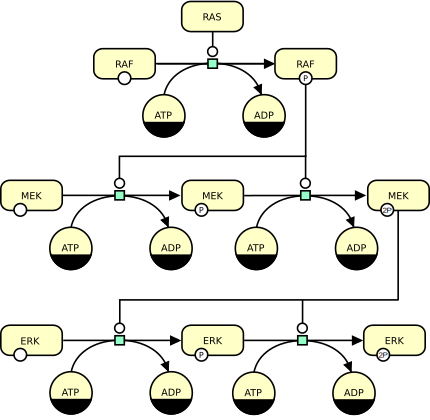
\includegraphics[scale=0.8]{images/MAPK-only}
  \caption{This example of a \PD uses two kinds of entity pool nodes: one for pools of different macromolecules (\sect{macromolecule}) and another for pools of simple chemicals (\sect{simpleChemical}). Most macromolecule nodes in this map are adorned with state variables (\sect{stateVariable}) representing phosphorylation states. This map uses one type of process node, the process node (\sect{process}), and three kind of connecting arc, consumption (\sect{consumption}), production (\sect{production}) and catalysis (\sect{catalysis}).  Finally, some entity pool nodes have dark bands along their bottoms; these are clone markers (\sect{cloneMarker}) indicating that the same pool nodes appear multiple times in the map.}
  \label{fig:eg1}
\end{figure}

The essence of the \PDs is \emph{change}: it shows how different entities in the system process from one form to another.  The entities themselves can be many different things.  In the example of \fig{eg1}, they are either pools of macromolecules or pools of simple chemicals, but as will become clear later in this chapter, they can be other conceptual and material constructs as well.  Note also that we speak of \emph{entity pools} rather than individuals; this is because in biochemical network models, one does not focus on single molecules, but rather collections of molecules of the same kind.  The molecules in a given pool are considered indistinguishable from each other.  The way in which one type of entity is transformed into another is conveyed by a \emph{process node} and arcs between entity pool nodes and process nodes indicate an influence by the entities on the processes.  In the case of \fig{eg1}, those arcs describe consumption (\sect{consumption}), production (\sect{production}) and catalysis
(\sect{catalysis}), but others are possible.  Finally, nodes in \PDs are usually not repeated; if they do need to be repeated, they are marked with \emph{clone markers}---specific modifications to the appearance of the node (\sect{cloneMarker}). The details of this and other aspects of \PD notation are explained in the rest of this chapter.

A reference card depicting all the symbols of \SBGNPDLone is present at the end of this document.

Lets look at a few additional examples which show typical biological processes and their SBGN \PD representation. In \fig{eg2} a reversible reaction with two substrates and one product is shown. The enzyme E catalyzes an irreversible (metabolic) process which consumes two substrates (S1 and S2) and produces one product (P1). The enzyme is a protein, therefore represented as a \emph{macromolecule}. Substrates and product of the biochemical reaction are represented by \emph{simple chemicals}. The consumption of S1 and S2 is represented by the \emph{consumption arcs}. The \emph{production arc} represents the synthesis of P1. 

In \fig{eg3} the formation of a complex is shown. Two \emph{macromolecule} entities X and Y form the \emph{complex} X\underline{ }Y. Complex formation is represented using the \emph{association} process node with ingoing \emph{consumption} and outgoing \emph{production} arcs. The \emph{complex} glyph surrounds subunits X and Y.

\begin{figure}[h]
  \centering
  \vspace*{-0.75em}
  \includegraphics[scale=0.5]{images/Fig12}
  \caption{This example of a \PD shows an irreversible catalysis with 2 substrates and 1 products.}
  \label{fig:eg2}
\end{figure}

\begin{figure}[h]
  \centering
  \vspace*{-0.75em}
  \includegraphics[scale=0.5]{images/Fig13}
  \caption{This example of a \PD shows an irreversible catalysis with 2 substrates and 1 products.}
  \label{fig:eg3}
\end{figure}

In \fig{eg4} the regulation of a target gene by a transcription factor without knowledge about the promoter binding is shown. A transcription factor (TF) protein together with a target gene promoter X triggers the\emph{process} of transcription. Direct binding of the TF to the target gene promoter has not been experimentally verified, therefore the \emph{logical operator} AND is used to describe the yet unspecified interaction between TF and target gene. The TF protein is a \emph{macromolecule} of the \emph{material type} 'protein' (mt:prot) whereas the gene promoter is given as a \emph{nucleic acid feature} with the \emph{conceptual type} 'gene' (ct:gene). The connecting arc \emph{necessary stimulation} is applied to indicate that the stimulation by both regulator and target is necessary for the transcription process to take place. The target gene messenger as a product of the transcription process is represented by a \emph{nucleic acid feature} with the \emph{conceptual type} 'mRNA' (ct:mRNA). The \emph{unspecified source} symbol is used to represent the large number of substrates of a transcription process (i.e. trinucleotides).

A last example is show in \fig{eg5}, which shows passive transport or diffusion of a molecule. The \emph{macromolecule} X in the cytosol serves as the substrate of a process leading to the production of the \emph{macromolecule} X in the nucleus. This process describes the passive transport of X from one \emph{compartment} to the other. The two macromolecules X do not carry the clone marker because the containing compartment is part of their identity.

More examples can be found in a list of so called SBGN bricks~\cite{Junker:2012}, which are building blocks representing basic biological patterns. These bricks can be used for assembly into different kinds of biological networks such as metabolic and regulatory networks.

\begin{figure}[h]
  \centering
  \vspace*{-0.75em}
  \includegraphics[scale=0.5]{images/Fig14}
  \caption{This example of a \PD shows a regulation of a target gene by a transcription factor without knowledge about the promoter binding.}
  \label{fig:eg4}
\end{figure}


\begin{figure}[h]
  \centering
  \vspace*{-0.75em}
  \includegraphics[scale=0.5]{images/Fig15}
  \caption{This example of a \PD shows a passive transport of a molecule.}
  \label{fig:eg5}
\end{figure}

\section{SBGN levels and versions}
\label{sec:sbgn-levels}

It was clear at the outset of SBGN development that it would be impossible to design a perfect and complete notation right from the beginning.  Apart from the prescience this would require (which, sadly, none of the authors possess), it also would likely need a vast language that most newcomers would shun as being too complex.  Thus, the SBGN community followed an idea used in the development of other standards, i.e. stratify language development into levels.

A \emph{level} of one of the SBGN languages represents a set of features deemed to fit together cohesively, constituting a usable set of functionality that the user community agrees is sufficient for a reasonable set of tasks and goals.  Within \emph{levels}, \emph{versions} represent small evolution of a language, that may involve new glyphs, refined semantics, but no fundamental change of the way maps are to be generated and interpreted. In addition new versions should be backwards compatible, \ie \PD maps that conform to an earlier version of the \PDl within the same level should still be valid.  This does not apply to new levels.

Capabilities and features that cannot be agreed upon and are judged insufficiently critical to require inclusion in a given level, are postponed to a higher level or version.  In this way, the development of SBGN languages is envisioned to proceed in stages, with each higher levels adding richness compared to the levels below it.

\section{How to get more information}
\label{sec:info}

This user manual will present the various symbols used by \SBGNPDLone (\chap{symbols}), and provide guidance to design SBGN \PDms (\chap{build}). The authors tried to keep the presentation simple, and to avoid being too technical.

The normative description of the language is the technical specification \cite{Moodie:2011}. It is available from the SBGN website (\url{http://sbgn.org/}). This website is a portal for all things to the notation. In addition to the specifications, there are examples of maps, FAQs, and informations on part and forthcoming meetings.

The easiest and best way to get involved in SBGN  discussions is to join the \href{mailto://sbgn-discuss@caltech.edu}{sbgn-discuss@caltech.edu} mailing list. If you only want the announcements of meetings and new specifications, you can join the very low flux mailing list \href{mailto://sbgn-announce@lists.sf.net}{sbgn-announce@lists.sf.net} instead.

% $HeadURL$

\chapter{Concepts and Glyphs}
\label{chp:glyphs}


\section{Introduction}

Although ultimately defined by its glyphs, \SBGNPDLone these glyphs
represent concepts that are related to varying degrees and ultimately
can be organised hierarchically. This provides us with a useful way or
organising the glyphs and thinking about \PD{}.  Therefore in this
chapter we describe the conceptual structure of \SBGNPDLone and place
each glyph within this structure. For each glyph or concept we describe its
physical appearance and define syntax and other usage rules. An
overview of this hierarchy is provided in figure
\ref{fig:sbgn_node_tax}.

\begin{figure}[htb]
\begin{center}
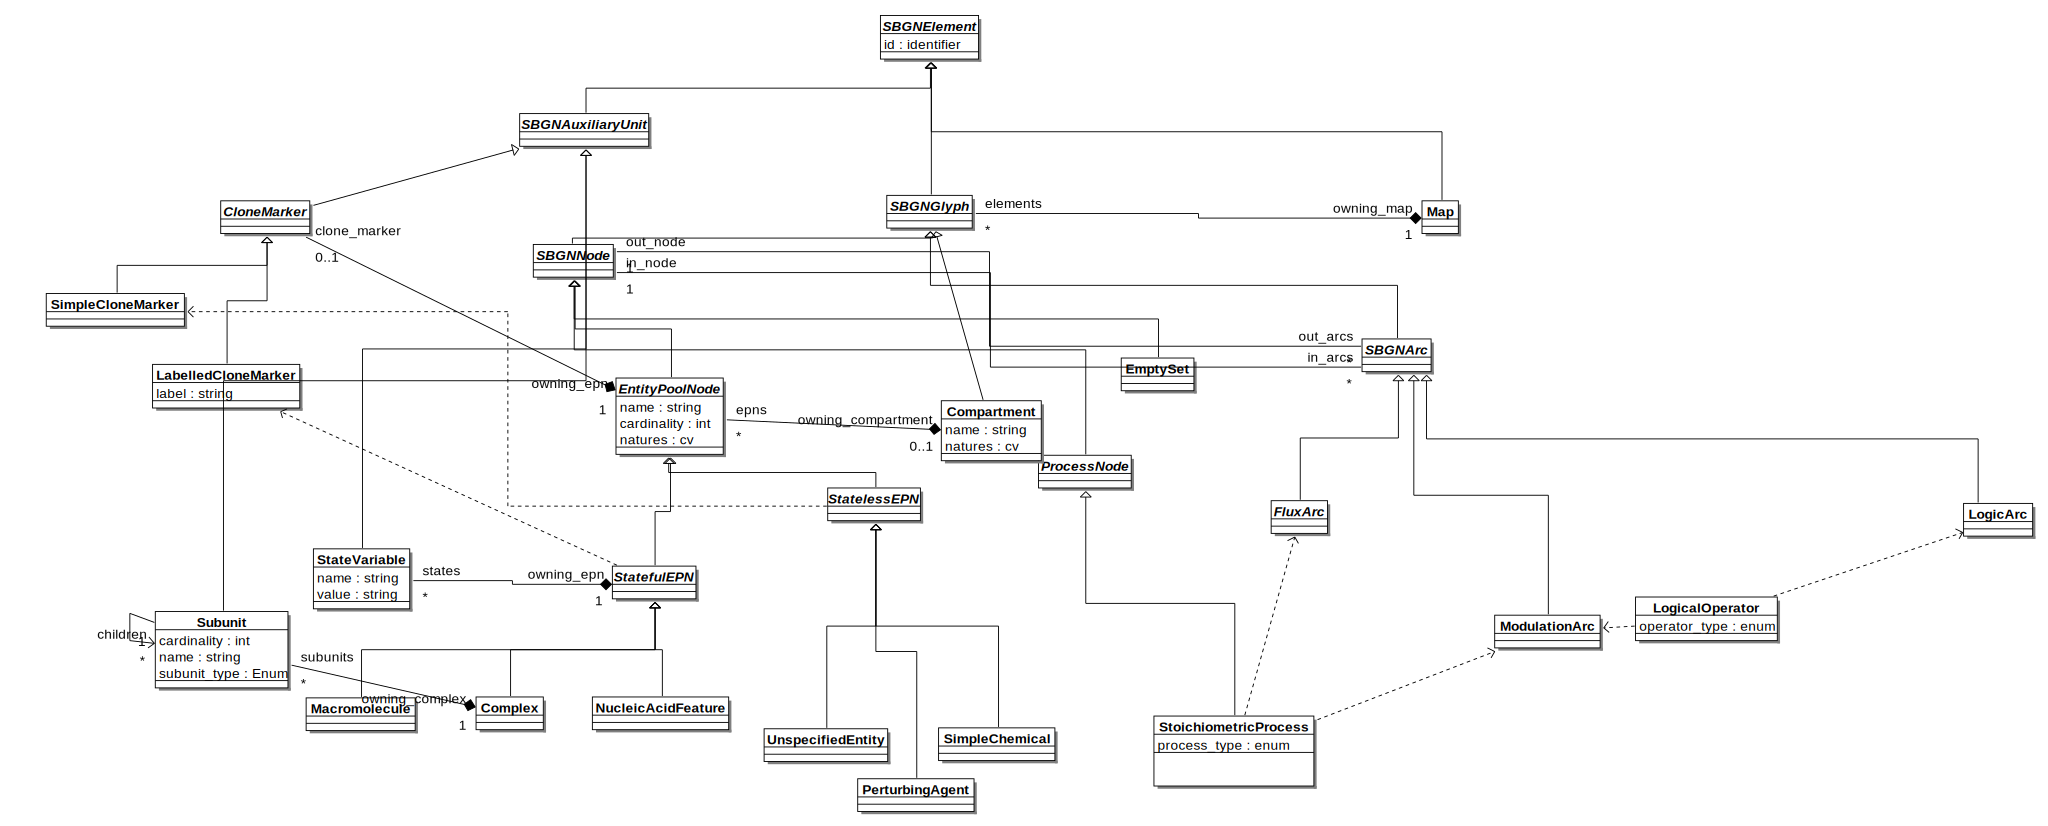
\includegraphics[width=1.0\linewidth]{images/sbgnumloverview}
\caption{Organisation of the node glyphs within SBGN \PDl. All UML classes (boxes) correspond to \PD node glyphs except those with italicised names, which are organisational groupings. They correspond to the groupings used elsewhere in this document.}
\label{fig:sbgn_node_tax}
\end{center}
\end{figure}


\section{How to read the Language Specification}

\begin{itemize}
\item Organised alphabetically.
\item use UML to describe the language elements.
\item Some language elements decribe concepts and rules, some
  describe elements that are represented by glyphs, other both.
\item Class represent concepts.
\item Classes have attributes which are required (R), optional (O), or can be
  a collection of a number of values. In the latter case the permitted
  of range is specified as:
  \begin{description}
  \item[*] any number
  \item[1..*] 1 or more
  \end{description}
\item Associations are indicated by solid lines. If there is a black
  diamont then this means the class the diamond is closest to contains
  the other class. This means the contained class cannot exist without
  the parent class, \ie if the containing class instance is destroyed
  then the contained is too.
\item open diamonds are a referencing association, the referenced
  class can exist without the refernecing class.
\item dependency indicates that there is an indirect association
  between these classes.
\item direction containment or referencing means that one side see the
  other, but the other does not see the refernecing class.
\item cardinality on the edges of the class refer to the distrant
  class and indicate the follwoing:
  \begin{description}
  \item[1] mandatory that one instance is associated.
  \item[*] optional - any number of instances permited in association
  \item[1..*] mandatroy that at least 1 is associated
  \item[0..1] Optional. instance is optional.
  \end{description}
  \item class defines all possible cases
  \item instance is a single case of the class with attributes and
    associates set. In SBGN case a glyph is an instance of a class.
  \item Idea is that UML defines language elements and then the
    notation sections specifies the graphical
    representation. Equivalent to the grammar of a language and the
    letters used to write it.
  \item aim is to minimise duplication of rules as much as possible to
    improve maintainability. Compromised between that and readability
    and ease of understanding spec.
\end{itemize}

\section{Definitions}
\label{sec:definitions}

\subsection{SBGNElement}
\label{defn:SBGNElement}

All the glyphs in \SBGNPDLone inherit from
\sbgnclass{SBGNElement}. This is an abstract or conceptual class that
helps organise \PD conceptually. \sbgnclass{SBGNElement} (figure
\ref{fig:mapuml}) has a single attribute \attrib{id} that is an
identifying attribute. This means that all SBGN elements defined here,
which ultimately extend \sbgnclass{SBGNBase}, can all be uniquely
identified from each other. This makes sense if you think that a glyph
drawn on a map is distinct from another glyph drawn on the map. The
\attrib{id} attribute reflects this and is not shown explicitly in a
\PDm.


\subsubsection{Generalisation}

None

\subsubsection{Attributes}

\begin{attributes}
  \attitem{id}{identifier}{R} uniquely identified all SBGN elements in
  the same namespace.
\end{attributes}

\subsubsection{Changes from Previous Version}

Not defined in the previous version.

\subsection{Map}
\label{defn:Map}\label{sec:map}


\begin{figure}[h!]
  \centering
  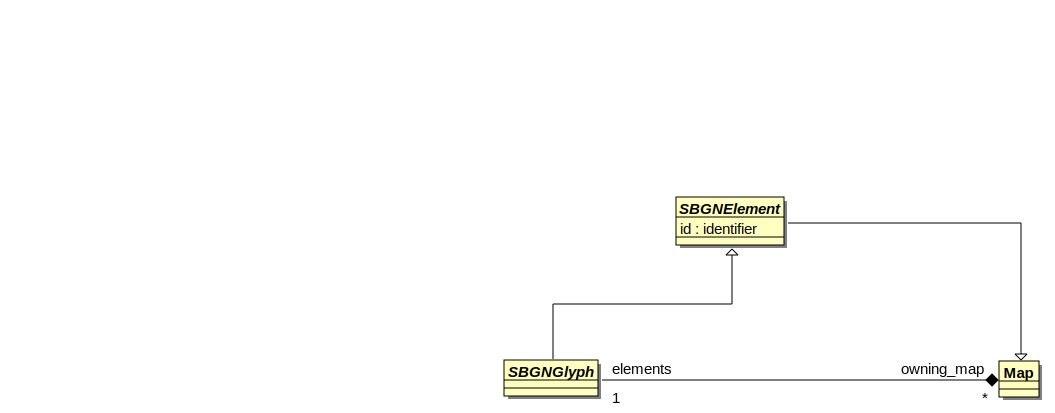
\includegraphics[width=0.75\textwidth]{images/mapuml}
  \caption{UML definition of Map and \sbgnclass{SBGNElement}.}
  \label{fig:mapuml}
\end{figure}

The \sbgnclass{Map} (figure \ref{fig:mapuml}) is a container that
holds all the glyphs drawn in a \PDm. A \sbgnclass{Map} may contain a
\classref{SubmapNode} in which case some of the detail is summarised
in another \PDm. In this case the former is referred to as the ``Main
Map'' and the latter the ``Submap''. A Main Map shares the same
namespace as its Submap and uses the \classref{CrossReference}
identify the interface between both maps. The details of Main Map and
Submap linking semantics are described in more detail in section
\ref{sec:submaplinkingsemantics}.


\subsubsection{Generalisation}

\begin{itemize}
\item \classref{SBGNElement}
\end{itemize}

\subsubsection{Attributes}

No additional attributes

\subsubsection{Associations}

\begin{attributes}
\associtem{elements}{SBGNGlyph}{*} The collection of glyphs held by the map. 
\end{attributes}

\subsubsection{Rules and Constraints}

\begin{itemize}
\item A map is valid if it is empty (although not very useful).
\item All instances of \classref{SBGNGlyph} must be unique (see
  section \ref{sec:uniquenessdefinition}).
\end{itemize}

\subsubsection{Notation}

The map is the canvas upon which the \PDl is drawn. It's only visible
feature is its colour. It can take any pattern or colour (or be
transparent for that matter), but as SBGN is `colour blind' this does
not convey any meaning in itself.

\subsubsection{Changes from Previous Version}

Not defined explicitly in previous versions.

\subsection{SBGNGlyph}
\label{defn:SBGNGlyph}

\begin{figure}[htb]
  \centering
  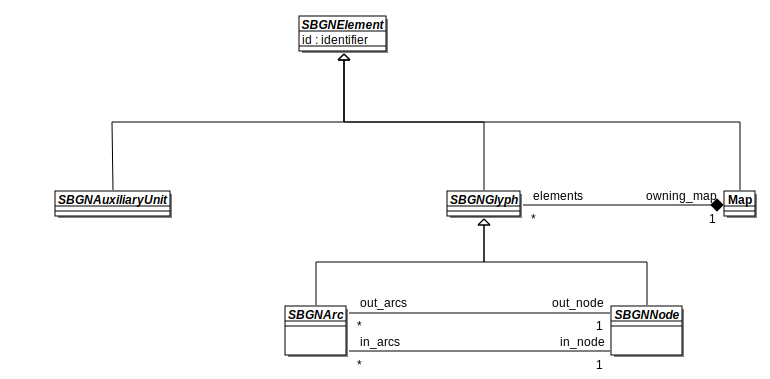
\includegraphics[width=0.75\textwidth]{images/glyphauxuml}
\caption{UML definition of the Auxiliary Unit and its subclasses.}
  \label{fig:glyphauxuml}
\end{figure}

 Glyphs are the fundamental building blocks of the \PDl and are the
only elements that can be drawn directly on a map (\sbgnclass{Map}).

\subsubsection{Generalisation}

\begin{itemize}
\item \classref{SBGNElement}
\end{itemize}

\subsubsection{Attributes}

No additional attributes.

\subsubsection{Associations}

\begin{attributes}
\associtem{owning\_map}{Map}{1} The map that contains this class.
\end{attributes}

\subsubsection{Rules and Constraints}

No additional rules and constraints.

\subsubsection{Changes from Previous Version}

Not defined in  previous version.


\subsection{AuxiliaryUnit}
\label{defn:AuxiliaryUnit}

\begin{figure}[htb]
  \centering
  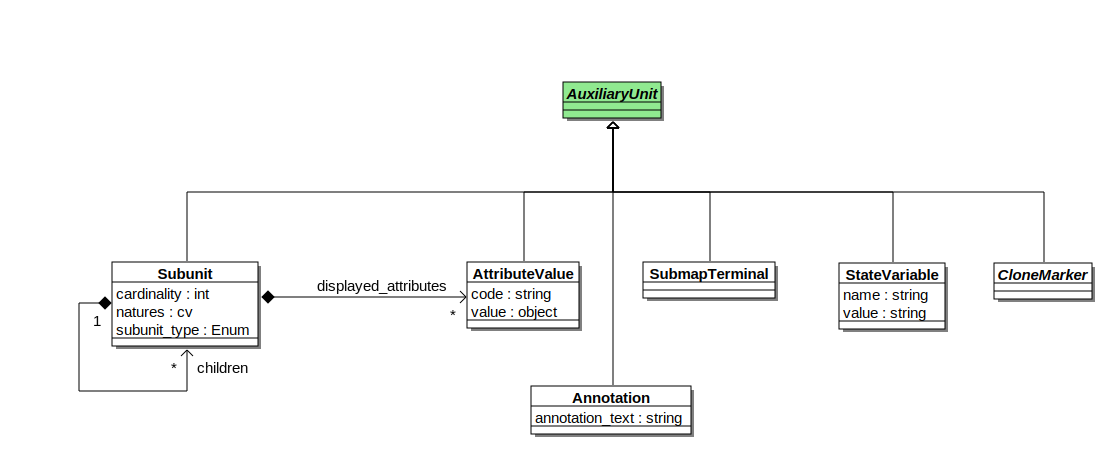
\includegraphics[width=0.75\textwidth]{images/auxiliaryunituml}
\caption{UML definition of the Auxiliary Unit and its subclasses.}
  \label{fig:auxiliaryunituml}
\end{figure}

 The \sbgnclass{AuxiliaryUnit} (figure \ref{fig:auxiliaryunituml}) represents symbols that may be used to
adorn glyphs. In doing so they change the meaning of the glyph and/or provide
additional information about it.

\subsubsection{Generalisation}

\begin{itemize}
\item \classref{SBGNElement}
\end{itemize}

\subsubsection{Attributes}

No additional attributes.

\subsubsection{Associations}

No additional associations.

\subsubsection{Rules and Constraints}

No additional rules and constraints.

\subsubsection{Changes from Previous Version}

Not defined in previous version.


\subsection{SBGNNode}
\label{defn:SBGNNode}

The \sbgnclass{SBGNNode} (figure \ref{fig:glyphauxuml}) represents the nodes in the graph structure
that is the core representation within \PDl. The nodes are connected
to glyphs descended from \sbgnclass{SBGNArc} for form a direct graph.

\subsubsection{Generalisation}

\begin{itemize}
\item \classref{SBGNGlyph}
\end{itemize}

\subsubsection{Attributes}

No additional attributes.

\subsubsection{Associations}

\begin{attributes}
  \associtem{out\_arcs}{SBGNArc}{*} The arcs that are leaving this node.
  \associtem{in\_arcs}{SBGNArc}{*} The arcs that are entering this node.
\end{attributes}
 
\subsubsection{Rules and Constraints}

No additional rules and constraints.

\subsubsection{Changes from Previous Version}

Not defined in the previous version.

\subsection{SBGNArc}
\label{defn:SBGNArc}

The \sbgnclass{SBGNArc} (figure \ref{fig:glyphauxuml}) represents the arcs (also know as edges) in
the graph structure that is the core representation within \PDl. The
arc is connected to two nodes descended from \sbgnclass{SBGNNode}, one
at each end. As the arc has a direction (directed arc) these nodes are
by convention designated the \emph{out node} to indicate the arc is
leaving the node and \emph{in node} to indicate that it is entering
the node.

\subsubsection{Generalisation}

\begin{itemize}
\item \classref{SBGNGlyph}
\end{itemize}

\subsubsection{Attributes}

No additional attributes.

\subsubsection{Associations}

\begin{attributes}
  \associtem{out\_node}{SBGNNode}{1} The node that this arc is leaving.
  \associtem{in\_node}{SBGNNode}{1} The node that this arc is entering.
\end{attributes}

\subsubsection{Rules and Constraints}

No additional rules and constraints.

\subsubsection{Changes from Previous Version}

Not defined in the previous version.


\subsection{EntityPoolNode}
\label{sec:EPNs}\label{defn:EntityPoolNode}\label{sec:EPN}

An entity pool is a population of entities that cannot be
distinguished from each other, when it comes to the \SBGNPDLone
map. For instance all the molecular entities that fulfill the same
role in a given process form an entity pool. As a result, an entity
pool can represent different granularity levels, such as all the
proteins, all the instances of a given protein, only certain forms of
a given protein. To belong to a different compartment is sufficient to
belong to different entity pools. Calcium ions in the endoplasmic
reticulum and calcium ions in the cytosol belong to different entity
pools when it comes to representing calcium release from the
endoplasmic reticulum.

% The \PD contains five glyph types representing classes of material
% entities: \glyph{unspecified entity} (\sect{unspecifiedEntity}),
% \glyph{simple chemical} (\sect{simpleChemical}), \glyph{macromolecule}
% (\sect{macromolecule}), \glyph{nucleic acid feature} (\sect{genetic})
% and \glyph{complex} (\sect{complex}).  (Specific types of
% macromolecules, such as protein, RNA, DNA, polysaccharide, and
% specific simple chemicals are not defined by \PD but may be part of
% future levels of SBGN.)  In addition to the material entities, \PD
% represents a conceptual entities: \glyph{perturbing agent} (\sect{perturbing
%   agent}).

\begin{figure}[htb]
  \centering
  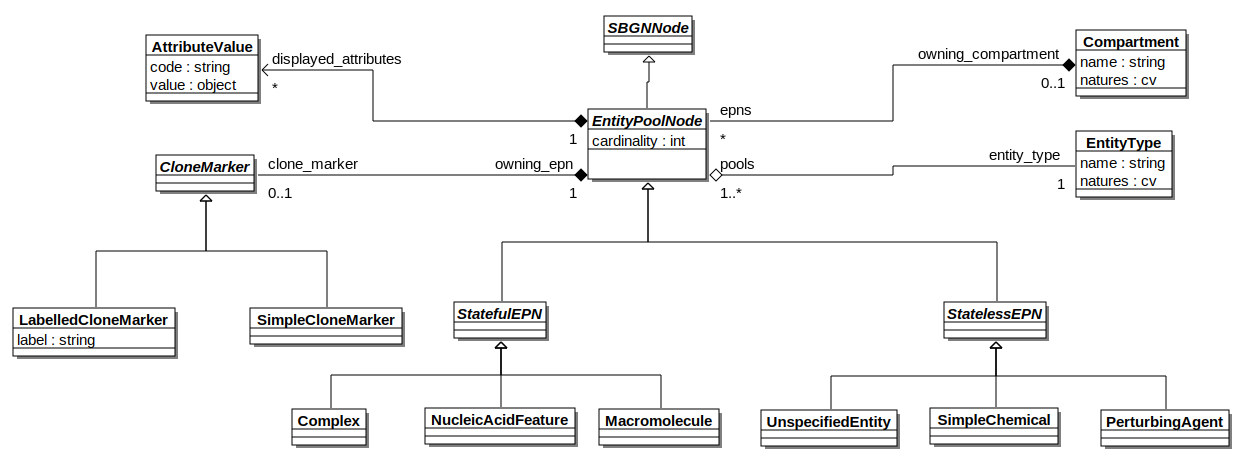
\includegraphics[width=0.85\textwidth]{images/epnuml}
\caption{UML definition of the entity pool node and its descendant glyphs.}
  \label{fig:epnuml}
\end{figure}
 
The \sbgnclass{EntityPoolNode} (figure \ref{fig:epnuml}) is the common
ancestor of all these glyphs and defines attributes that are common to
all its descendants. It must belong to a compartment (c.f.\, section
\ref{sec:compartment})  and can contain a clone marker if it is
cloned. Note that not all EPNs can be cloned.

\subsubsection{Generalisation}

\begin{itemize}
\item \classref{SBGNNode}
\end{itemize}

\subsubsection{Attributes}

\begin{attributes}
  \attitem{label}{string}{R} The name that identifies the entity in the
  \PDm. EPNs with the same label should be from the same entity. the
  string cannot be empty and must start and end with a non-space
  character. Any Unicode character is acceptable.
  \attitem{cardinality}{int}{R} The number of copies of the entity. Must
  be a positive non-zero integer.
  \attitem{natures}{cv}{O} The nature of the entity pool node as defined
  by a controlled vocabulary. Zero, one or more values may be set, but
  each one must belong to a different controlled vocabulary.
\end{attributes}

\subsubsection{Associations}

\begin{attributes}
 \associtem{owning\_compartment}{Compartment}{0..1} The compartment
  that this EPN belongs too.
  \associtem{clone\_marker}{CloneMarker}{0..1} The clone marker
  decorator. See section \ref{sec:cloneMarker} for its use.
 \associtem{displayed\_attributes}{AttributeValue}{*} One or
 more decorators used to display attribute values.
\end{attributes}

\subsubsection{Logical Identity}

\begin{logicalkey}
\item \attrib{owning\_compartment}
\item \attrib{name}
\item \attrib{cardinality}
\item \attrib{natures}
\end{logicalkey}

\subsubsection{Rules and Constraints}

\begin{itemize}
\item If \attrib{cardinality} $>1$ then the descendant glyph must be displayed
  as a multimer.
\item If the EPN is drawn directly on a \glyph{Map} then
 \attrib{owning\_compartment} is assigned to an invisible default
 compartment.
 \attrib{nature} can only use the material type (section
 \ref{sec:material-types-cv}), conceptual type (section \ref{sec:conceptual-types-cv}) or physical
 characteristics (section \ref{sec:physical-characteristics-cv}) controlled vocabularies.
\item The appropriate subclass of \sbgnclass{CloneMarker} must be used
  to distinguish logically identical instances of this class.
\end{itemize}

\subsubsection{Notation}

Although there is no direct graphical representation of this class
this class does affect the appearance of the
\sbgnclass{AttributeValue} and its associated glyph the \glyph{Unit of
  Information}. The \glyph{Unit of Information} can be used to present
the \attrib{cardinality} and \attrib{natures} attributes. These used
the following codes to indicate which attribute is being presented''

\begin{center}
  \begin{itemize}\setlength{\parskip}{0ex}
  \item[\texttt{pc}] container physical characteristic
  \item[\texttt{mt}] entity pool material type
  \item[\texttt{ct}] entity pool conceptual type
  \item[\texttt{N}]  multimer cardinality
  \end{itemize}
\end{center}


\subsubsection{Changes from Previous Version}

Not defined in the previous version.

\subsection{Empty Set}
\label{sec:sourceSink}

It is useful to have the ability to represent the creation of an entity or
a state from an unspecified source, that is, from something that one does
not need or wish to make precise.  For instance, in a model where the
production of a protein is represented, it may not be desirable to
represent all of the amino acids, sugars and other metabolites used, or the
energy involved in the protein's creation.  Similarly, we may not wish to
bother representing the details of the destruction or decomposition of some
biochemical species into a large number of more primitive entities,
preferring instead to simply say that the species ``disappears into a
sink''.  Yet another example is that one may need to represent an input
(respectively, output) into (resp. from) a compartment without explicitly
representing a transport process from a source (resp. to a target).

For these and other situations, SBGN defines a single glyph to handle
these situations representing the involvement of an external pool of entities.  The symbol
used in SBGN is borrowed from the mathematical symbol for ``empty set'',
but it is important to note that it does not actually represent a true
absence of everything or a physical void---it represents the absence of the
corresponding structures in the model, that is, the fact that the
external pool is conceptually outside the scope of the map.

A frequently asked question is, why bother having an explicit symbol at
all?  The reason is that one cannot simply use an arc that does not
terminate on a node, because the dangling end could be mistaken to be
pointing to another node in the map.  This is specially true if the
map is rescaled, causing the spacing of elements in the map to
change.  The availability and use of an explicit symbol for sources and
sinks is critical.

\begin{figure}[htb]
  \centering
  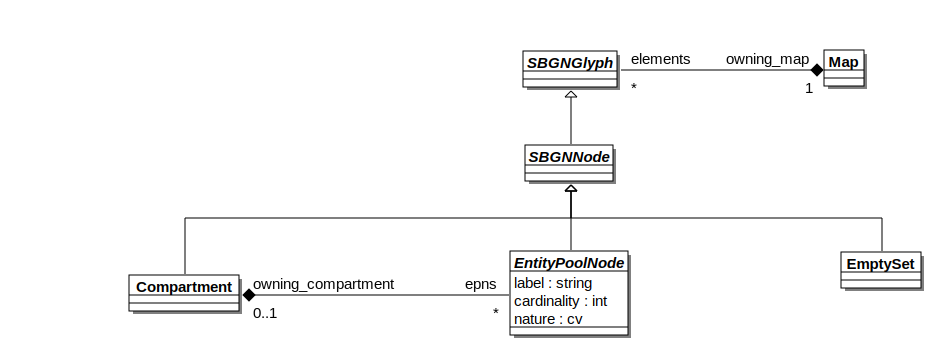
\includegraphics[width=0.75\textwidth]{images/emptysetuml}
  \caption{The UML definition of the \glyph{EmptySet} and its context
    in relation to other elements of the \PDl.}
  \label{fig:emptysetuml}
\end{figure}

The definition of the \glyph{Empty Set} is shown in figure
\ref{fig:emptysetuml}. The empty set is not an EPN as it does not
represent a single pool of entities and does not share any of the
other attributes of an EPN, nor does it belong to a particular
compartment.

\subsubsection{Generalisation}

\begin{itemize}
\item \classref{SBGNNode}
\end{itemize}

\subsubsection{Attributes}

No additional attributes.

\subsubsection{Associations}

No additional associations.

\subsubsection{Rules and Constraints}

\begin{itemize}
\item  All instances of \glyph{Empty Set} can be regarded as identical
therefore not special decoration is used to indicate replication on
the map.
\end{itemize}

\subsubsection{Notation}

\paragraph{Glyph: \glyph{Empty Set}}

\begin{figure}[H]
  \centering
  
\includegraphics[width = 0.1\textwidth]{images/sourceSink}
  \caption{The \glyph{empty set} glyph.}
  \label{fig:sourceSink}
\end{figure}

\begin{glyphDescription}
\glyphSboTerm SBO:0000291 ! empty set
\glyphAux None
\glyphContainer Represented by the mathematical symbol for ``empty
set'', that is, a circle crossed by a bar linking the upper-right and
lower-left corners of an invisible square drawn around the circle ($\emptyset$).
\fig{sourceSink} illustrates this.  The symbol should be linked to one
and only one edge in a map.
\glyphLabel None
\end{glyphDescription}

\subsubsection{Changes from Previous Version}

The \sbgnclass{EmptySet} and \glyph{Empty Set} glyph has replaced the \glyph{Source} and
\glyph{Sink} glyphs. This symbols used remains the same, but the
underlying concept has changed. The \glyph{Source} and \glyph{Sink}
glyphs where types of EPN.

\subsection{StatelessEPN}
\label{defn:StatelessEPN}

The \sbgnclass{StatelessEPN} (figure \ref{fig:statelessepnuml})
represents a pool where the entities do not change `state'. In
other-words the entities do not undergo any physical change that is
useful to record in a \PDm. Therefore these glyphs cannot be assigned
a state-variable.

\begin{figure}[htb]
  \centering
  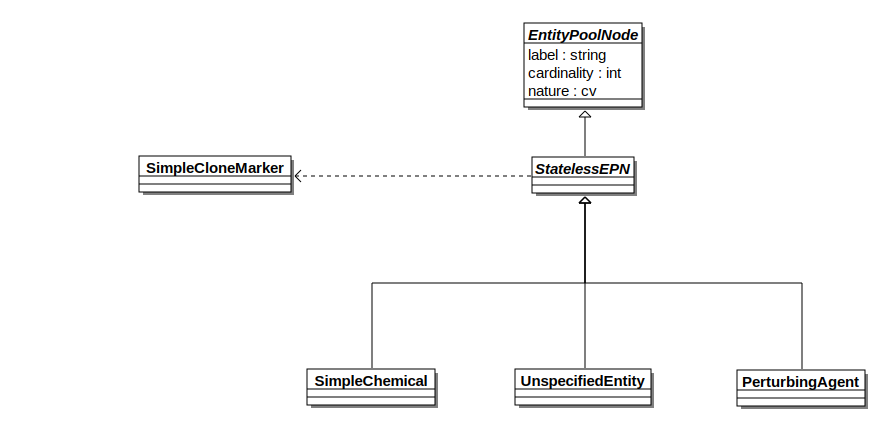
\includegraphics[width=0.75\textwidth]{images/statelessepnuml}
\caption{UML definition of the stateless entity pool node and its descendant glyphs.}
  \label{fig:statelessepnuml}
\end{figure}

\subsubsection{Generalisation}

\begin{itemize}
\item \classref{EntityPoolNode}
\end{itemize}

\subsubsection{Attributes}

No additional attributes.

\subsubsection{Associations}

No additional associations.

\subsubsection{Rules and Constraints}

\begin{itemize}
\item if a clone marker is used it must be of type \sbgnclass{SimpleCloneMarker}.
\end{itemize}

\subsubsection{Changes from Previous Version}

Not defined in the previous version.

\subsection{Simple chemical}
\label{sec:simpleChemical}

A simple chemical in SBGN is defined as the opposite of a
macromolecule (\sect{macromolecule}): it is a chemical compound that
is \emph{not} formed by the covalent linking of pseudo-identical
residues.  Examples of simple chemicals are an atom, a monoatomic ion,
a salt, a radical, a solid metal, a crystal, etc. The complex can be
represented by a monomeric glyph (\glyph{Simple chemical monomer}) and
a multimeric glyph (\glyph{Simple chemical multimer}).

\subsubsection{Generalisation}

\begin{itemize}
\item \classref{StatelessEPN}
\end{itemize}

\subsubsection{Attributes}

No additional attributes.

\subsubsection{Associations}

No additional associations.

\subsubsection{Rules and Constraints}

No additional rules and constraints.

\subsubsection{Notation}

\paragraph{Glyph: \glyph{Simple chemical monomer}}

\begin{figure}[htb]
  \centering
  
\includegraphics[scale = 0.3]{images/simpleChemical}
  \caption{The \PD glyph for \glyph{simple chemical}.}
  \label{fig:simpleChemical}
\end{figure}

\begin{glyphDescription}
\glyphSboTerm SBO:0000247 ! simple chemical
\glyphContainer A \glyph{simple chemical} is represented by a circular
container, as depicted in \fig{simpleChemical}. To avoid confusion
with the Unspecified Entity (\ref{sec:unspecifiedEntity}), this glyph
must remain a circle and cannot be deformed into an eclipse.
\glyphLabel The identification of the \glyph{simple chemical} is carried by an unbordered box containing a string of characters.  The characters may be distributed on several lines to improve readability, although this is not mandatory.  The label box has to be attached to the center of the circular container.  The label is permitted to spill outside the container.
\glyphAux 
\end{glyphDescription}

\paragraph{Glyph: \glyph{Simple chemical multimer}}

\begin{figure}[htb]
  \centering
  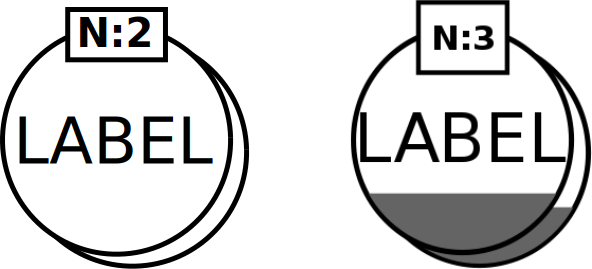
\includegraphics[scale = 0.3]{images/simpleChemicalMultimer}
  \caption{The \PD glyph for \glyph{multimer}.}
  \label{fig:multimer}
\end{figure}

\begin{glyphDescription}
\glyphSboTerm SBO:0000421 ! multimer of simple chemicals
\glyphContainer  A \glyph{simple chemical multimer} is represented by two identical containers shifted horizontally and vertically and stacked one on top of the other.  \fig{multimer} illustrates the glyph.
\glyphLabel A \glyph{multimer} has no identity on its own.  However, the first of the monomers carries an identifying label.  The label is placed in an unbordered box containing a string of characters.  The characters can be distributed on several lines to improve readability, although this is not mandatory.  The label box must be attached to the center of the top monomer's container.  The label may spill outside of the container.
\glyphAux 
\end{glyphDescription}

\subsubsection{Changes from Previous Version}

The glyphs used for the \sbgnclass{SimpleChemical} have been
changed. Previously the glyph was a circle.

\subsection{UnspecifiedEntity}
\label{sec:unspecifiedEntity}

The simplest type of EPN is the \sbgnclass{UnspecifiedEntity}: one whose
type is unknown or simply not relevant to the purposes of the map.
This arises, for example, when the existence of the entity has been
inferred indirectly, or when the entity is merely a construct
introduced for the needs of a map, without direct biological
relevance.  These are examples of situations where the
\sbgnclass{UnspecifiedEntity} is appropriate.  (Conversely, for
cases where the identity of the entities composing the pool \emph{is}
known, there exist other, more specific glyphs described elsewhere in
the specification.)

\subsubsection{Generalisation}

\begin{itemize}
\item \classref{StatelessEPN}
\end{itemize}

\subsubsection{Attributes}

No additional attributes.

\subsubsection{Associations}

No additional associations.

\subsubsection{Rules and Constraints}

\begin{itemize}
\item The \sbgnclass{UnspecifiedEntity} cannot have cardinality $>
  1$. This means there is no multimer glyph.
\end{itemize}

\subsubsection{Notation}

\paragraph{Glyph: \glyph{Unspecified entity}}

\begin{glyphDescription}
\glyphSboTerm SBO:0000285 ! material entity of unspecified nature 
\glyphContainer An \glyph{unspecified entity} is represented by an
elliptic container, as shown in \ref{fig:unspecified}.  Note that this
must remain an ellipse to avoid confusion with the Simple Chemical
glyph, which is a circle (c.f.\, \ref{sec:simpleChemical}).
\glyphLabel An \glyph{unspecified entity} is identified by a label
placed in an unbordered box containing a string of characters.  The
characters can be distributed on several lines to improve readability,
although this is not mandatory.  The label box must be attached to the
center of the container.  The label may spill outside of the
container.
\end{glyphDescription}

\begin{figure}[H]
  \centering
  \includegraphics[width=2.5in]{images/unspecified}
  \caption{The \PD glyph for \glyph{unspecified entity}.}
  \label{fig:unspecified}
\end{figure}

\subsubsection{Changes from Previous Version}

No changes from the previous version.

\subsection{Perturbing Agent}
\label{sec:perturbing agent}

Biochemical networks can be affected by external influences.  Those
influences can be the effect of well-defined physical perturbing
agents, such as a light pulse or a change in temperature; they can
also be more complex and not well-defined phenomena, for instance the
outcome of a biological process, an experimental setup, or a mutation.
For these situations, SBGN provides the \glyph{perturbing agent}
glyph. It is an EPN, and represents the amount to perturbing agent
applied to a process.

\subsubsection{Generalisation}

\begin{itemize}
\item \classref{StatelessEPN}
\end{itemize}

\subsubsection{Attributes}

No additional attributes.

\subsubsection{Associations}

No additional attributes.

\subsubsection{Rules and Constraints}

\begin{itemize}
\item The \sbgnclass{PerturbingAgent} cannot have \attrib{cardinality} $>
  1$. This means there is no multimer glyph.
\end{itemize}

\subsubsection{Notation}

\paragraph{Glyph: \glyph{Perturbing agent}}

\begin{figure}[H]
  \centering
  
\includegraphics[scale = 0.3]{images/perturbing_agent}
  \caption{The \PD glyph for \glyph{perturbing agent}.}
  \label{fig:perturbing agent}
\end{figure}

\begin{glyphDescription}
\glyphSboTerm SBO:0000405 ! perturbing agent
\glyphContainer A \glyph{perturbing agent} is represented by a modified hexagon
having two opposite concave faces, as illustrated in \fig{perturbing agent}.
\glyphLabel A \glyph{perturbing agent} is identified by a label placed in an
unbordered box containing a string of characters.  The characters can be
distributed on several lines to improve readability, although this is not
mandatory.  The label box must be attached to the center of the
\glyph{perturbing agent} container.  The label may spill outside of the container.
% \glyphAux A \glyph{perturbing agent} can optionally carry one or more \glyph{units of information} (\sect{unitInfo}).
% \glyphRules%
% \begin{inparaenum}
% \item A \glyph{perturbing agent} can optionally carry one or more \glyph{units of information} (\sect{unitInfo}).  A controlled vocaulary is available to describing the physical characteristic of the perturbing agent (see \sect{physical-characteristics-cv}).  
% \end{inparaenum}
% \glyphCloning Yes
\end{glyphDescription}

\subsubsection{Changes from Previous Version}

No changes from pervious version.

\subsection{StatefulEPN}
\label{defn:StatefulEPN}

Stateful entity pools can undergo physical changes, for example
chemical modifcation or conformational change, which we wish to record
in a \PDm. This information is captured via the
\sbgnclass{StateVariable}, as can be seen in figure
\ref{fig:statefulepnuml}). Replicated \sbgnclass{StatefulEPS}s are
indicated by the \glyph{Labelled Clone Marker} decoration. Note that
not all glyphs that are descendants of \sbgnclass{StatefulEPN} can be
cloned at all.

\begin{figure}[htb]
  \centering
  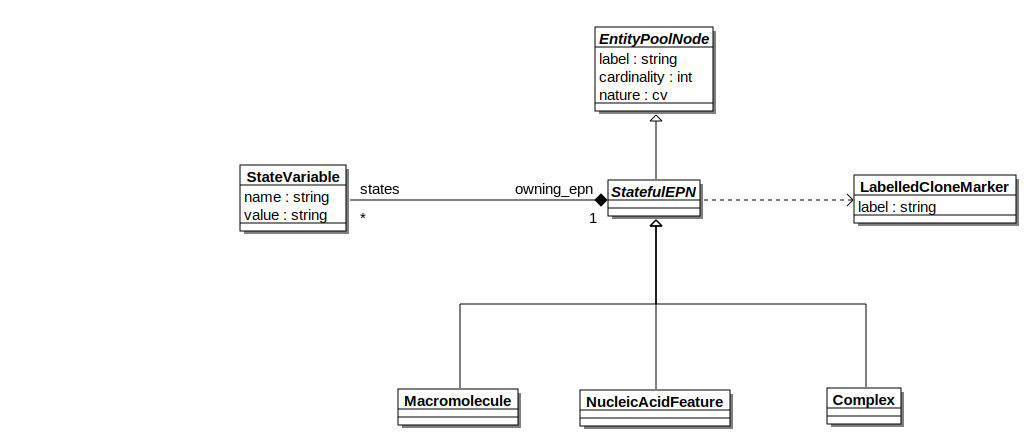
\includegraphics[width=0.75\textwidth]{images/statefulepnuml}
\caption{UML definition of the stateful entity pool node and its
  descendant glyphs and its association with state variables.}
  \label{fig:statefulepnuml}
\end{figure}

\subsubsection{Generalisation}

\begin{itemize}
\item \classref{EntityPoolNode}
\end{itemize}

\subsubsection{Attributes}

No additional attributes.

\subsubsection{Associations}

\begin{itemize}
\associtem{states}{StateVariable}{*} The state variables
  associated with this EPN.
\end{itemize}

\subsubsection{Rules and Constraints}

\begin{itemize}
\item Two or more state variables with the same name are
  permitted.
\item State variables with no name set are permitted.
\item A \sbgnclass{LabelledCloneMaker} must be used to indicate
  cloning.
\item \sbgnclass{StatefulEPN}s that are identical and so decorated
  with a \sbgnclass{LabelledCloneMarker} must use the same 
  label to indicate that they are part of the same `clone'.
\end{itemize}

\subsubsection{Changes from Previous Version}

Not defined in the previous version.

\subsection{Macromolecule}
\label{sec:macromolecule}

Many biological processes involve \emph{macromolecules}: biochemical
substances that are built up from the covalent linking of
pseudo-identical units.  Examples of macromolecules include proteins,
nucleic acids (RNA, DNA), and polysaccharides (glycogen, cellulose,
starch, etc.).  Attempting to define a separate glyph for all of these
different molecules would lead to an explosion of symbols in SBGN, so
instead, \SBGNPDLone defines only one glyph for all macromolecules.
The same glyph is to be used for a protein, a nucleic acid, a complex
sugar, and so on.  The exact nature of a particular macromolecule in a
map is then clarified using its label and decorations, as will become
clear below.  (Future levels of SBGN may subclass the
\glyph{macromolecule} and introduce different glyphs to differentiate
between types of macromolecules). This has two associated glyphs. One
where 

\subsubsection{Generalisation}

\begin{itemize}
\item \classref{StatefulEPN}
\end{itemize}

\subsubsection{Attributes}

No additional attributes.

\subsubsection{Associations}

No additional associations.

\subsubsection{Rules and Constraints}

No additional rules and constraints.

\subsubsection{Notation}

There are two glyphs associated with \sbgnclass{Macromolecule}. The
first \glyph{Macromolecule monomer} is used when \attrib{cardinality} $= 1$
and the second \glyph{Macromolecule multimer} is used when
\attrib{cardinality} $> 1$.

\paragraph{Glyph: \glyph{Macromolecule monomer}}

\begin{figure}[H]
  \centering
  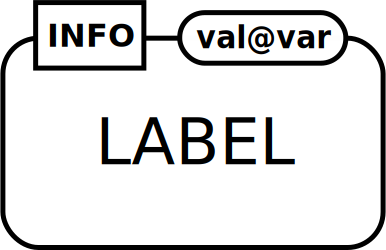
\includegraphics[width = 3in]{images/macromolecule}
  \caption{The \PD glyph for \glyph{macromolecule}, shown plain and
    unadorned on the left, and with with an additional state variable and a
    unit of information in the right and the cloned form on the right.}
  \label{fig:macromolecule}
\end{figure}

\begin{glyphDescription}
\glyphSboTerm SBO:0000245 ! macromolecule 
\glyphContainer A macromolecule is represented by a rectangular container with rounded
corners, as illustrated in \fig{macromolecule}.
\glyphLabel A \glyph{macromolecule} is identified by a label placed in an unbordered box containing a string of characters.  The characters can be distributed on several lines to improve readability, although this is not mandatory.  The label box must be attached to the center of the container.  The label may spill outside of the container.
\end{glyphDescription}

\paragraph{Glyph: \glyph{Macromolecule multimer}}

\begin{figure}[H]
  \centering
  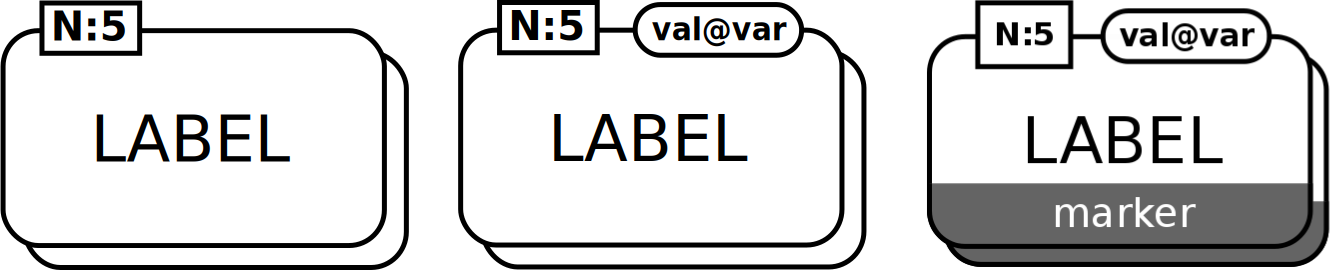
\includegraphics[width = 3.0in]{images/macromolMultimer}
  \caption{The \PD glyph for \glyph{macromolecule multimer}, shown plain and
    unadorned on the left, and with with an additional state variable and a
    unit of information on the right.}
  \label{fig:macromolMultimer}
\end{figure}

\begin{glyphDescription}
\glyphSboTerm SBO:0000420 ! multimer of macromolecules
\glyphContainer A \glyph{multimer} is represented by two identical containers shifted horizontally and vertically and stacked one on top of the other.  \fig{macromolMultimer} illustrates the glyph.
\glyphLabel As monomer
\end{glyphDescription}

\subsubsection{Changes from Previous Version}

No changes from the previous version.

\subsection{NucleicAcidFeature}
\label{sec:genetic}

The \sbgnclass{NucleicAcidFeature} represents a fragment of a macromolecule carrying genetic information.
A common use for this construct is to represent a gene or transcript.
The label of this EPN and its \attrib{nature} are often
important for making the purpose clear to the reader of a map.

\subsubsection{Generalisation}

\begin{itemize}
\item \classref{StatefulEPN}
\end{itemize}

\subsubsection{Attributes}

No additional attributes.

\subsubsection{Associations}

No additional associations.

\subsubsection{Rules and Constraints}

No additional rules and constraints.

\subsubsection{Notation}

The \sbgnclass{NucleicAcidFeature} has two associated glyphs. The
first \glyph{Nucleic acid feature monomer} is used when
\attrib{cardinality} $=1$ and the second, \glyph{Nucleic acid feature
  multimer} is used when \attrib{cardinality} $>1$.

\paragraph{Glyph: \glyph{Nucleic acid feature monomer}}

This glyphs represents a monomeric macromolecule.

\begin{glyphDescription}
\glyphSboTerm SBO:0000354 !  informational molecule segment
\glyphContainer A \glyph{nucleic acid feature} is represented by a rectangular container whose bottom half has rounded corners, as shown in \fig{genetic}. This design reminds that we are fundamentally dealing with a unit of information, but this information is carried by a macromolecule.
\glyphLabel The identity of a particular \glyph{Nucleic acid feature} is established by a label placed in an unordered box containing a string of characters.  The characters may be distributed on several lines to improve readability, although this is not mandatory.  The label box must be attached to the center of the container.  The label may spill outside of the container.
%\glyphAux A \glyph{nucleic acid feature} can carry state variables (\sect{stateVariable}) that add information about its precise state.  The state of a \glyph{nucleic acid feature} is therefore defined as the vector of all its state variables. 

%A \glyph{nucleic acid feature} can also carry one or several \glyph{units of information} (\sect{unitInfo}).  These can characterize a \glyph{nucleic acid feature}'s domain, such as a binding site, or an exon.  Particular \glyph{units of information} carry the material type (\sect{material-types-cv}) and the conceptual type (\sect{conceptual-types-cv}) of the \glyph{nucleic acid feature}. 

%\glyphCloning Labeled Clone Marker

\end{glyphDescription}


\begin{figure}[H]
  \centering
  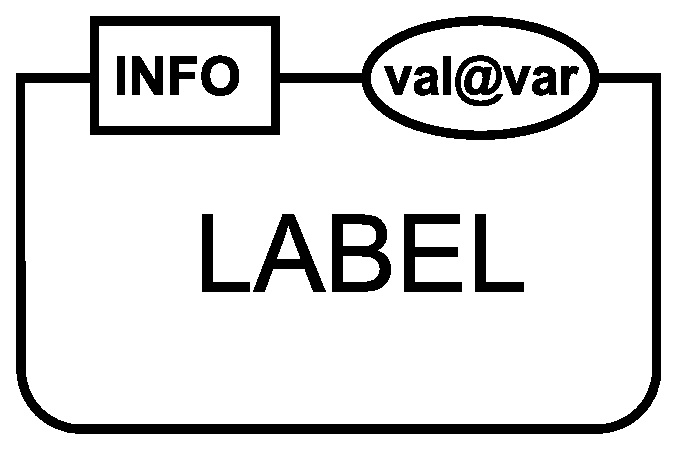
\includegraphics[width = 3in]{images/genetic}
  \caption{The \PD glyph for \glyph{nucleic acid feature monomer}, shown plain and
    unadorned on the left and with an additional state variable and a
    unit of information in the middle and the cloned form on the right.} 
  \label{fig:genetic}
\end{figure}

\paragraph{Glyph: \glyph{Nucleic acid feature multimer}}

This glyphs represents a multimeric macromolecule.

\begin{glyphDescription}

\glyphSboTerm SBO:0000419 ! multimer of informational molecule segments 

\glyphContainer A \glyph{Nucleic acid feature multimer} is represented by two identical containers shifted horizontally and vertically and stacked one on top of the other.  \fig{multimer} illustrates the glyph.

\glyphLabel As monomer glyph.

%\glyphAux A \glyph{nucleic acid feature} can carry state variables (\sect{stateVariable}) that add information about its precise state.  The state of a \glyph{nucleic acid feature} is therefore defined as the vector of all its state variables. 

%A \glyph{nucleic acid feature} can also carry one or several \glyph{units of information} (\sect{unitInfo}).  These can characterize a \glyph{nucleic acid feature}'s domain, such as a binding site, or an exon.  Particular \glyph{units of information} carry the material type (\sect{material-types-cv}) and the conceptual type (\sect{conceptual-types-cv}) of the \glyph{nucleic acid feature}. 

%A \glyph{nucleic acid feature} may also carry a \glyph{clone marker}
%(\sect{cloneMarker}).

\end{glyphDescription}

\begin{figure}[H]
  \centering
  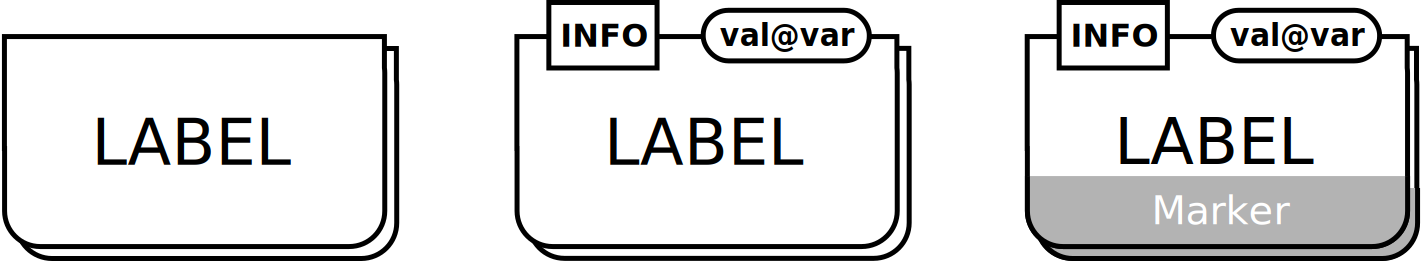
\includegraphics[width = 3in]{images/geneticMultimer}
  \caption{The \PD glyph for \glyph{nucleic acid feature multimer}, shown plain and
    unadorned on the left and with an additional state variable and a
    unit of information in the middle and the cloned form on the right.} 
  \label{fig:genetic-multimer}
\end{figure}

\subsubsection{Changes from Previous Version}

No changes from the previous version.

%%%%%%%%%%%%%%%%%%%%%%%%%%%%%%%%%%%%%%%%%%%%%%%%%%%%%%%%%%%%%%%%%%%%%%
%%%%                   Complex
%%%%%%%%%%%%%%%%%%%%%%%%%%%%%%%%%%%%%%%%%%%%%%%%%%%%%%%%%%%%%%%%%%%%%%

\subsection{Complex}\label{sec:complex}
\label{defn:Complex}

A \sbgnclass{Complex} represents a biochemical entity composed of
other biochemical entities, whether macromolecules, simple chemicals,
multimers, or other complexes (figure
\ref{fig:complexsubunituml}). The \sbgnclass{Complex} can described
its composition by the set of \sbgnclass{Subunit}s it contains (see
figure \ref{sec:subunits}). This description is entirely optional and
is their to assist the user with a visual shorthand about the
composition of the complex.

\begin{figure}[htb]
  \centering
  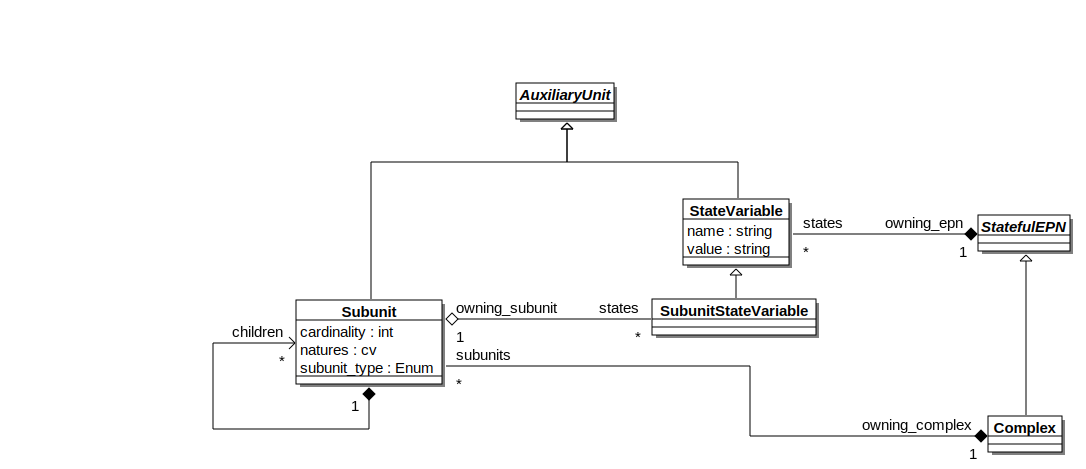
\includegraphics[width = 0.65\textwidth]{images/complexsubunituml}
  \caption{The UML definition of the \sbgnclass{Complex} and its
    associated \sbgnclass{subunit}s. In particular this describes organisation
   of the state variables that belong to both the subunit, but also
   the complex.}
  \label{fig:complexsubunituml}
\end{figure}

\subsubsection{Generalisations}

\begin{itemize}
\item \classref{EntityPoolNode} 
\end{itemize}

\subsubsection{Attributes}

No additional attributes 

\subsubsection{Associations}

\begin{attributes}
  \associtem{subunits}{Subunit}{*} The subunits that describe
  the composition of this complex.
 \end{attributes}


\subsubsection{Special Rules and Constraints}

\begin{itemize}
\item Once a set of subunits are defined then they are always defined.
\item The set of subunits in the Complex does not identify it. One or
  more Complexes that contain the same set of subunits, but have
  different labels are \textbf{not} identical.
\end{itemize}

% \begin{glyphDescription}
% \glyphName \sbgnclass{Complex}
% \glyphSboTerm Not defined
% \begin{glyphIdentity}
%   \attitem{subunits}{\sbgnclass{Subunit}} The subunits that describe
%   the composition of this complex.
%  \end{glyphIdentity}
% \glyphRules
% \begin{itemize}
%   \item Once a set of subunits are defined then they are always
%     defined.
% \end{itemize}
% \end{glyphDescription}

\subsubsection{Notation}

The Complex is represented by two glyphs, the \glyph{Complex Monomer}
which represents a \sbgnclass{Complex} where the \attrib{cardinality}
is one and the \glyph{Complex Multimer} where the cardinality is
greater than that.

\paragraph{\glyph{Complex Monomer}}

\begin{figure}[H]
  \centering
  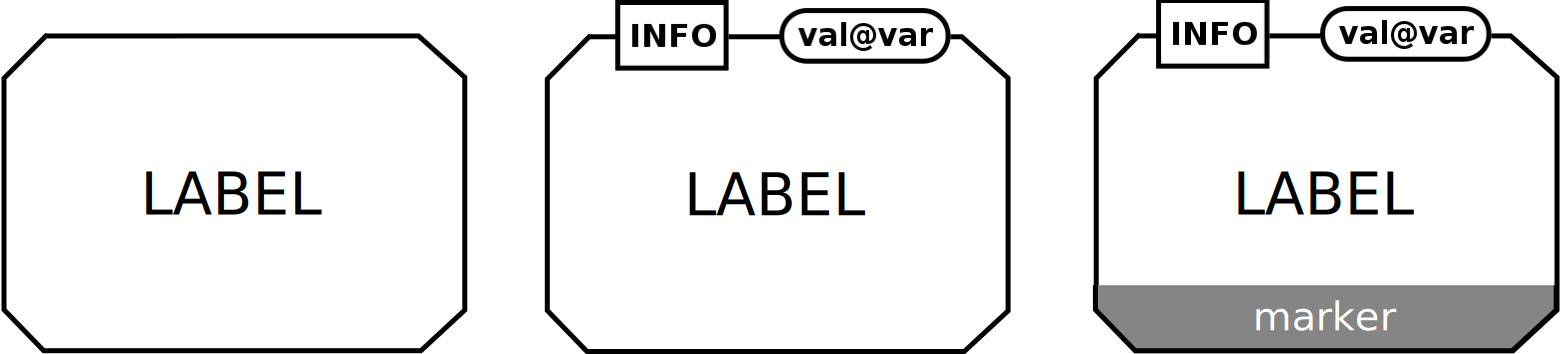
\includegraphics[width=3.5in]{images/complexGlyph}
  \caption{The \glyph{complex} glyph.}
  \label{fig:complex}
\end{figure}

\begin{glyphDescription}
\glyphSboTerm SBO:0000253 ! non-covalent complex
\glyphAux A \glyph{complex} can carry state variables (see \sect{stateVariable}).  The state of a complex is defined by the set of the all its state variable and all the state variables of all its components.  A \glyph{complex} can also carry one or several \glyph{units of information} (see \sect{unitInfo}). A \glyph{complex} may carry a \glyph{clone marker} (see \sect{cloneMarker}).
\glyphCloning Labeled Clone Marker
\glyphContainer A \glyph{complex} possesses its own container box surrounding the juxtaposed container boxes of its components.  This container box is a rectangle with cut-corners (an octagonal box with sides of two different lengths).  The size of the cut-corners are adjusted so that there is no overlap between the container and the components.  The container boxes of the components must not overlap.
\glyphLabel The identification of a \glyph{named complex} is carried
by an unbordered box containing a string of characters.  The
characters may be distributed on several lines to improve readability,
although this is not mandatory.  Ideally the label box should be
attached to the midway between the border of the complex's container
box and the border of the components' container boxes. However, if the
Complex contains Subunit glyphs then the label may be positions to
optimise the clarity and avoid overlapping.
\end{glyphDescription}


\paragraph{\glyph{Complex Multimer}}

\begin{figure}[H]
  \centering
  \includegraphics[width = 3.5in]{images/complexMultimerGlyph}
  \caption{The \glyph{Complex Multimer} glyph.}
  \label{fig:complexMultimer}
\end{figure}

 \begin{glyphDescription}
\glyphSboTerm SBO:0000418 ! multimer of complexes
\glyphAux As monomer.
\glyphCloning Labeled Clone Marker
\glyphContainer A \glyph{Complex Multimer} is represented by two
identical \glyph{Complex} containers shifted horizontally and
vertically and stacked one on top of the other.  \fig{complexMultimer}
illustrates the glyph.
\glyphLabel As monomer
\end{glyphDescription}

\paragraph{Examples of complex EPNs}
\label{sec:CplxEPNs}

In this section, we provide examples of Entity Pool Node representations drawn using the \SBGNPDLone glyphs described above. 

\fig{example-camkii} represents calcium/calmodulin kinase II, with phosphorylation on the sites threonine 286 and 306, as well as catalytic and autoinhibitory domains.  Note the use of \emph{units of information} and \emph{state variables}.

\begin{figure}[H]
  \centering
  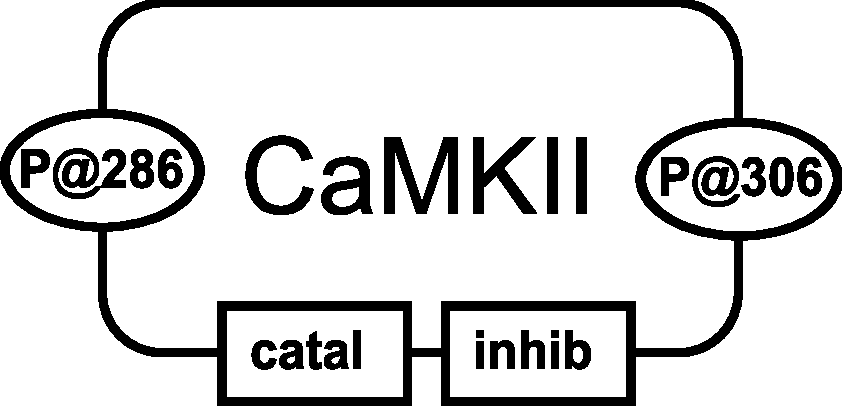
\includegraphics[scale = 0.3]{examples/macromolecule-CaMKII}
  \caption{An example representation of calcium/calmodulin kinase II.}
  \label{fig:example-camkii}
\end{figure}

\fig{example-glur} represents the glutamate receptor in the open state, with both phosphorylation and glycosylation.  The entity carries two functional domains, the ligand-binding domain and the ion pore, and its chemical nature is precided.

\begin{figure}[H]
  \centering
  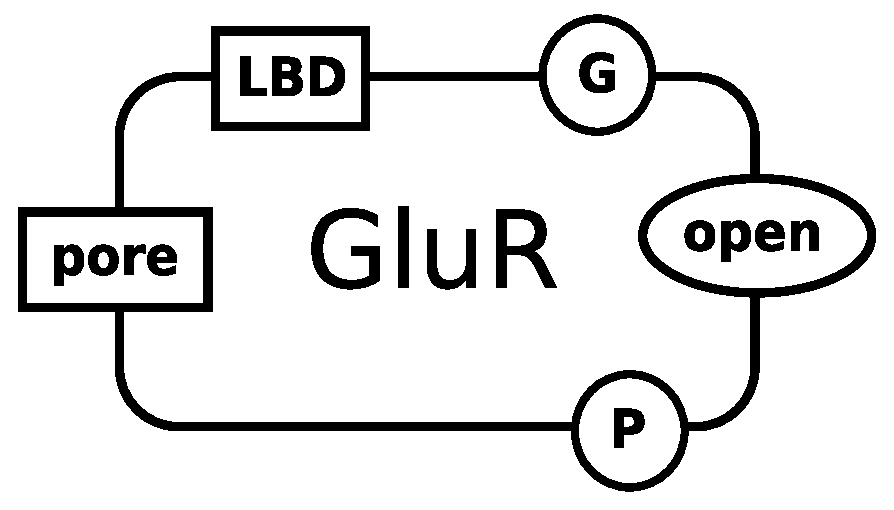
\includegraphics[scale = 0.3]{examples/macromolecule-GluR}
  \caption{An example of a glutamate receptor in the open state.}
  \label{fig:example-glur}
\end{figure}


\subsubsection{Layout Rules and Guidelines}

\begin{itemize}
\item The subunits inside the complex must not overlap.
\item The subunits should sit above the clone marker so that they are
  not obscured by it.
\item The label should not be obscured by subunits or obscure them.
\end{itemize}


\subsubsection{Changes from Previous Version}

\begin{itemize}
\item Clarified that complex must have a label and the label
  identifies the complex irrespective of its subunit composition.
\item The label positioning does not need to be at the centre of the
  Complex glyph.
\end{itemize}

\subsection{Subunit}
\label{defn:Subunit}\label{sec:subunits}

A complex can optionally be decorated with subunit symbols
(\sbgnclass{Subunit} see figure \ref{fig:complexsubunituml}) to
describe the composition of the complex. The symbols available are
equivalent to those used by the EPN glyphs including the
\glyph{complex}. Therefore it is possible to describe complexes within
complexes. Subunits may contain labels. 

\begin{center}
\tablecaption{Mapping between the subunit types and the glyphs used to
  represent it. These are essentially the EPN glyphs described in this document.}
\label{tab:subunit types}
\begin{footnotesize}
\tablefirsthead{\hline
  Subunit type & Monomer Glyph & Multimer Glyph\\\hline}
\tablehead{\hline
\multicolumn{3}{|l|}{\small\sl continued from previous page}\\
\hline\hline
  Subunit type & Monomer Glyph & Multimer Glyph\\\hline\hline}
\tabletail{\hline
\multicolumn{3}{|r|}{\small\sl continued on next page}\\
\hline}
\tablelasttail{\hline}
\begin{supertabular}{|l|l|l|}\hline
SimpleChemical &  \glyph{Simple Chemical Monomer} & \glyph{Simple
  Chemical Multimer}\\\hline
UnspecifiedEntity & \glyph{Unspecificed Entity} & None\\\hline
PerturbingAgent & \glyph{Perturbing Agent} & None\\\hline
Macromolecule & \glyph{Macromolecule Monomer} &
\glyph{Macromolecule Multimer}\\\hline
Nucleic\-Acid\-Feature & \glyph{Nucleic Acid Feature Monomer} & \glyph{Nucleic Acid Feature Multimer}\\\hline
Complex & \glyph{Complex Monomer} & \glyph{Complex Multimer}\\\hline
\end{supertabular}
\end{footnotesize}
\end{center}

\subsubsection{Generalisation}

\begin{itemize}
\item \classref{EntityPoolNode} 
\end{itemize}

\subsubsection{Attributes}

\begin{attributes}
  \attitem{cardinality}{int}{R} The number of copies of the subunit.
  \attitem{name}{string}{O} The name of the subunit.
  \attitem{subunit\_type}{enum}{R} The type of the subunit. It can have
  one of the following values that correspond to the equivalent EPN
  class: \sbgnclass{SimpleChemical}, \sbgnclass{UnspecifiedEntity},
  \sbgnclass{PerturbingAgent}, \sbgnclass{Macromolecule},
  \sbgnclass{NucleicAcidFeature}, \sbgnclass{Complex}.
\end{attributes}

\subsubsection{Associations}

\begin{attributes}
  \associtem{owning\_complex}{Complex}{1} The complex that owns the subunit.
  \associtem{states}{SubunitStateVariable}{*} The state variables assigned
  to this subunit.
  \associtem{children}{Subunit}{*} Subunits that are contained by this subunit.
\end{attributes}

\subsubsection{Rules and Constraints}

\begin{itemize}
\item Two or more state variables with the same name are
  permitted.
\item State variables with no name set are permitted.
\item Subunits can also contain subunits. There is no limit on such nesting. The namespace rules
  below apply.
\item Each state variable actually belongs to the Complex.
\item The subunit defines a namespace for its state variables, e.g.\,
  subunit ``A'' assigned a state variable ``P@Ser202''  and a subunit
  ``B'' assigned the same state variable can be distinguised as
  A:P@Ser202 and B:P@Ser202.
\item If the subunit is of type Complex then \attrib{children} can contain one or
  more \sbgnclass{Subunit} instances.
\item If the subunit has a cardinality $>1$ then this should be
  displayed by the \classref{AttributeValue}.
\item If \attrib{natures} contains one or more instances then these
  must be displayed via a \sbgnclass{AttributeValue}.
\end{itemize}

\subsubsection{Notation}

The example in figure \fig{complexSubunits} illustrates the use of
subunits in a complex shows an equivalent compex without
subunits. This is an import point. For every \glyph{Complex} drawn
with subunits it will always be possible to drawn an equivalent
version that does not use contains subunits.

\begin{figure}[H]
  \centering
  \includegraphics[width = 3.0in]{images/complex}
  \caption{Both these complex glyphs are equivalent. The one on the
    left is described using subunit decorators, the one on the right
    describes the same thing without them.}
  \label{fig:complexSubunits}
\end{figure}

\subsubsection{Changes from Previous Version}

%%%%%%%%%%%%
% Put the following in the semantics section

% \subsubsection{Attributes}


% The complex has the following attributes (those in \emph{italic} identify the complex):

% \begin{description}
% \item[\emph{name}]
% \item[\emph{cardinality}] The number of subunits of the complex. If
%   cardinality $> 1$ then the \glyph{Complex Multimer} must be
%   drawn. Otherwise a \glyph{Complex} is drawn. The cardinality is an
%   integer $>0$.
% \item[\emph{compartment}] The complex must belong to one compartment.
% \item[state variables] The complex can have zero, one or more state
%   variables. 
% \item[clone ID]
% \end{description}


%%%%%%%%%%%%%%%%%%%%%%%%%%%%%%%%%%%%%%%%%%%%%%%%%%%%%%%%%%%%%%%%%%%%%%
%%%%%%%%%%%%%%%%%%%%%%%%%%%%%%%%%%%%%%%%%%%%%%%%%%%%%%%%%%%%%%%%%%%%%%
%%%%                   Process nodes
%%%%%%%%%%%%%%%%%%%%%%%%%%%%%%%%%%%%%%%%%%%%%%%%%%%%%%%%%%%%%%%%%%%%%%
%%%%%%%%%%%%%%%%%%%%%%%%%%%%%%%%%%%%%%%%%%%%%%%%%%%%%%%%%%%%%%%%%%%%%%

\subsection{ProcessNode}\label{sec:PNs}
\label{defn:ProcessNode}

The \sbgnclass{Process} (figure \ref{fig:processumlview}) represents a process that transforms one or
more entity pools into one or more entity pools, that are identical or
different. A process may be used to represent or summarise more than
one known process.  \SBGNPDLone defines a generic \glyph{process}
(\sect{process}), as well as five more specific ones: the
\glyph{omitted process} (\sect{omitted}), the \glyph{uncertain
  process} (\sect{uncertain}), the \glyph{association}
(\sect{association}), the \glyph{dissociation} (\sect{dissociation}),
and the \glyph{phenotype} (\sect{phenotype}).

\begin{figure}[htb]
  \centering
  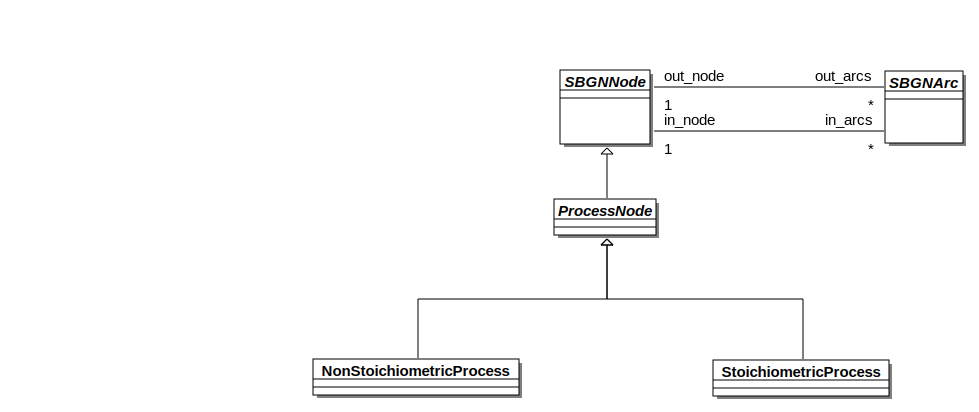
\includegraphics[width = 0.65\textwidth]{images/processumlview}
  \caption{The UML definition of the \sbgnclass{Process} and its
    associated subclasses. Note that the \sbgnclass{Process} extends
    \sbgnclass{SBGNNode} so all its descendants can potentially be
    nodes in a directed graph.}
  \label{fig:processumlview}
\end{figure}


\subsubsection{Generalisation}

\begin{itemize}
\item \classref{SBGNNode}
\end{itemize}

\subsubsection{Attributes}

No additional attributes.

\subsubsection{Associations}

No additional associations.

\subsubsection{Rules and Constraints}

No additional rules and constraints.

\subsubsection{Changes from Previous Version}
\begin{itemize}
\item This was not explicitly defined in the previous version, but
  this version did define a glyph called \glyph{Process}. To avoid
  ambiguity this glyph has now been renamed \glyph{Stoichiometric
    Process} (see section \ref{sec:stoichiometricprocess}).
\item Previous specifications stated that processed could be
  duplicated when all associated EPNs were cloned. This behaviour has
  been changed the current status where all processes are unique in a \PDm.
\end{itemize}

\subsection{NonStoichiometricProcess}
\label{defn:NonStoichiometricProcess}

The \sbgnclass{NonStoichiometricProcess} (figure
\ref{fig:nonstoichprocessuml}) is a type of process. It does not
necessarily result in a measurable change of entity pools, nor does it
necessarily have a defined start and end point. In many cases the
process is not well defined. This may because it is not well
understood or because the detail is not important or is being
summarised.

\begin{figure}[htb]
  \centering
  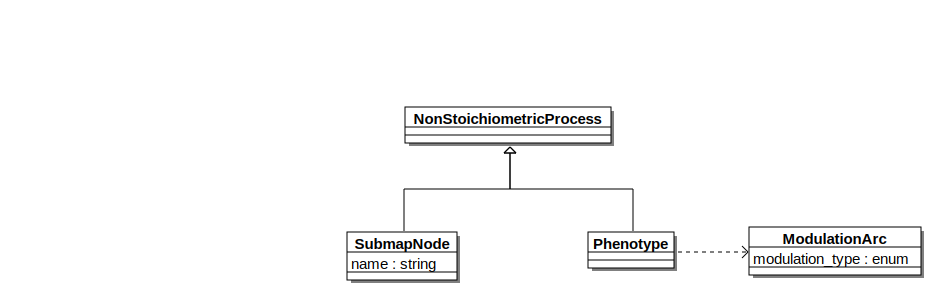
\includegraphics[width = 0.45\textwidth]{images/nonstoichprocessuml}
  \caption{The UML definition of the \sbgnclass{NonStoichiometricProcess} and its
    associated subclasses.}
  \label{fig:nonstoichprocessuml}
\end{figure}

\subsubsection{Generalisation}

\begin{itemize}
\item \classref{ProcessNode}
\end{itemize}

\subsubsection{Attributes}

No additional attributes.

\subsubsection{Associations}

No additional associations.

\subsubsection{Rules and Constraints}

No additional rules and constraints.

\subsubsection{Changes from Previous Version}

Not defined in the previous version.

\subsection{Phenotype}

A biochemical network can generate phenotypes or affect biological
processes.  Such processes can take place at different levels and are
independent of the biochemical network itself.  To represent these
processes in a map, SBGN defines the \sbgnclass{Phenotype} (figure \ref{fig:nonstoichprocessuml}).

\subsubsection{Generalisation}

\begin{itemize}
\item \classref{NonStoichiometricProcess}
\end{itemize}

\subsubsection{Attributes}

No additional attributes.

\subsubsection{Associations}

No additional associations.

\subsubsection{Rules and Constraints}

\begin{itemize}
\item The \sbgnclass{Phenotype} can only be modulated.
\item The \sbgnclass{Phenotype} must be connected to at least one
  modulating arc.
\end{itemize}

\subsubsection{Notation}

\paragraph{Glyph: \glyph{Phenotype}}
\label{sec:phenotype}

\begin{glyphDescription}

\glyphSboTerm SBO:0000358 ! phenotype

\glyphContainer A \glyph{phenotype} is represented by an elongated
hexagon, as illustrated in \fig{phenotype}.

\glyphLabel A \glyph{phenotype} is identified by a label placed in an
unbordered box containing a string of characters.  The characters can be
distributed on several lines to improve readability, although this is not
mandatory.  The label box must be attached to the center of the
\glyph{phenotype} container.  The label may spill outside of the container.
\end{glyphDescription}
 
\begin{figure}[H]
  \centering
  \includegraphics[scale = 0.3]{images/phenotype}
  \caption{The \PD glyph for \glyph{phenotype}.}
  \label{fig:phenotype}
\end{figure}


\subsubsection{Changes from Previous Version}

Clarified that the \sbgnclass{Phenotype} cannot be cloned as it is now
a subclass of \sbgnclass{Process}, which is always unique.


\subsection{SubmapNode}
\label{sec:submap}\label{defn:SubmapNode}

The \sbgnclass{SubmapNode} ( figure \ref{fig:submapnodeuml} ) is a
placeholder for another process and is used when one wishes to hide
the detail of this process from the \PDm, but make it available to the
reader as a separate related map. The \sbgnclass{Submap} is not
equivalent to an \sbgnclass{OmittedProcess} (section
\ref{sec:omitted}). The \sbgnclass{Submap} allows the detail of
section of the \PDm to be exported to another \PDm and replaced by the
\sbgnclass{SubmapNode}, which acts as a place-holder.  This is
described in section \ref{sec:map} and the semantics of submap linking
is defined in section \ref{sec:submaplinkingsemantics}.

\begin{figure}[htb]
  \centering
  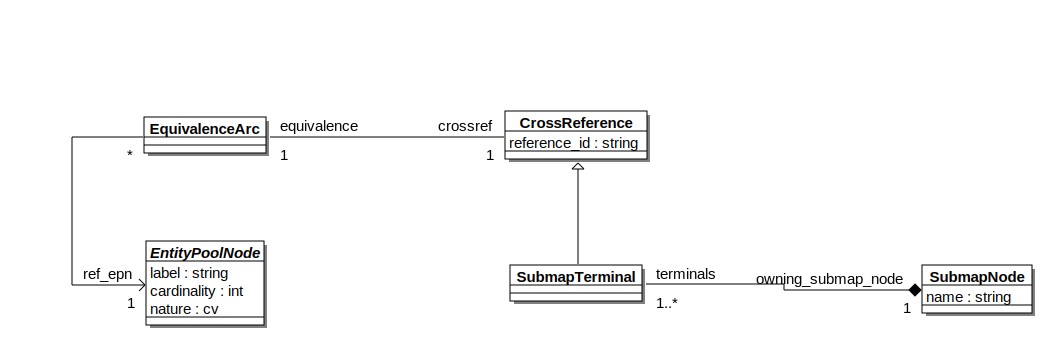
\includegraphics[width = 0.65\textwidth]{images/submapnodeuml}
  \caption{The UML definition of the \sbgnclass{SubmapNode} and its
   relationship to its submap, tags etc.}
  \label{fig:submapnodeuml}
\end{figure}

\subsubsection{Generalisation}

\begin{itemize}
\item \classref{NonStoichiometricProcess}
\end{itemize}

\subsubsection{Attributes}

\begin{attributes}
  \attitem{name}{string}{R} The name of the submap that is being
  summarised. Note that this name ideally will indicate the function
  or the processes that are being summarised.
\end{attributes}

\subsubsection{Associations}

\begin{attributes}
\associtem{terminals}{SubmapTerminal}{1..*} The terminals provide a
reference between the EPNs in the Main Map and those in the submap,
which are identified by a \sbgnclass{Tag}.
\end{attributes}

\subsubsection{Rules and Constraints}

\begin{itemize}
\item All instances of \classref{SubmapTerminal} held by this class
  must be unique.
\end{itemize}

\subsubsection{Notation}

\paragraph{Glyph: \glyph{Submap Node}}

\begin{glyphDescription}

\glyphSboTerm SBO:0000395 ! encapsulating process

\glyphContainer The \glyph{submap} is represented as a square box to remind the viewer that it is fundamentally a process.

\glyphLabel The identification of the \glyph{submap} is carried by an unbordered box containing a string of characters.  The characters may be distributed on several lines to improve readability, although this is not mandatory.  The label box has to be attached to the center of the container box.

\glyphAux A \glyph{submap} carries labeled terminals.  When the \glyph{submap} is represented folded, those terminals are linked to external \glyph{EPNs} (\sect{EPNs}).  In the unfolded view, exposing the internal structure of the \glyph{submap}, a set of \glyph{tags} point to the corresponding internal \glyph{EPNs} \sect{EPNs}.

\end{glyphDescription}


\begin{figure}[H]
  \centering
  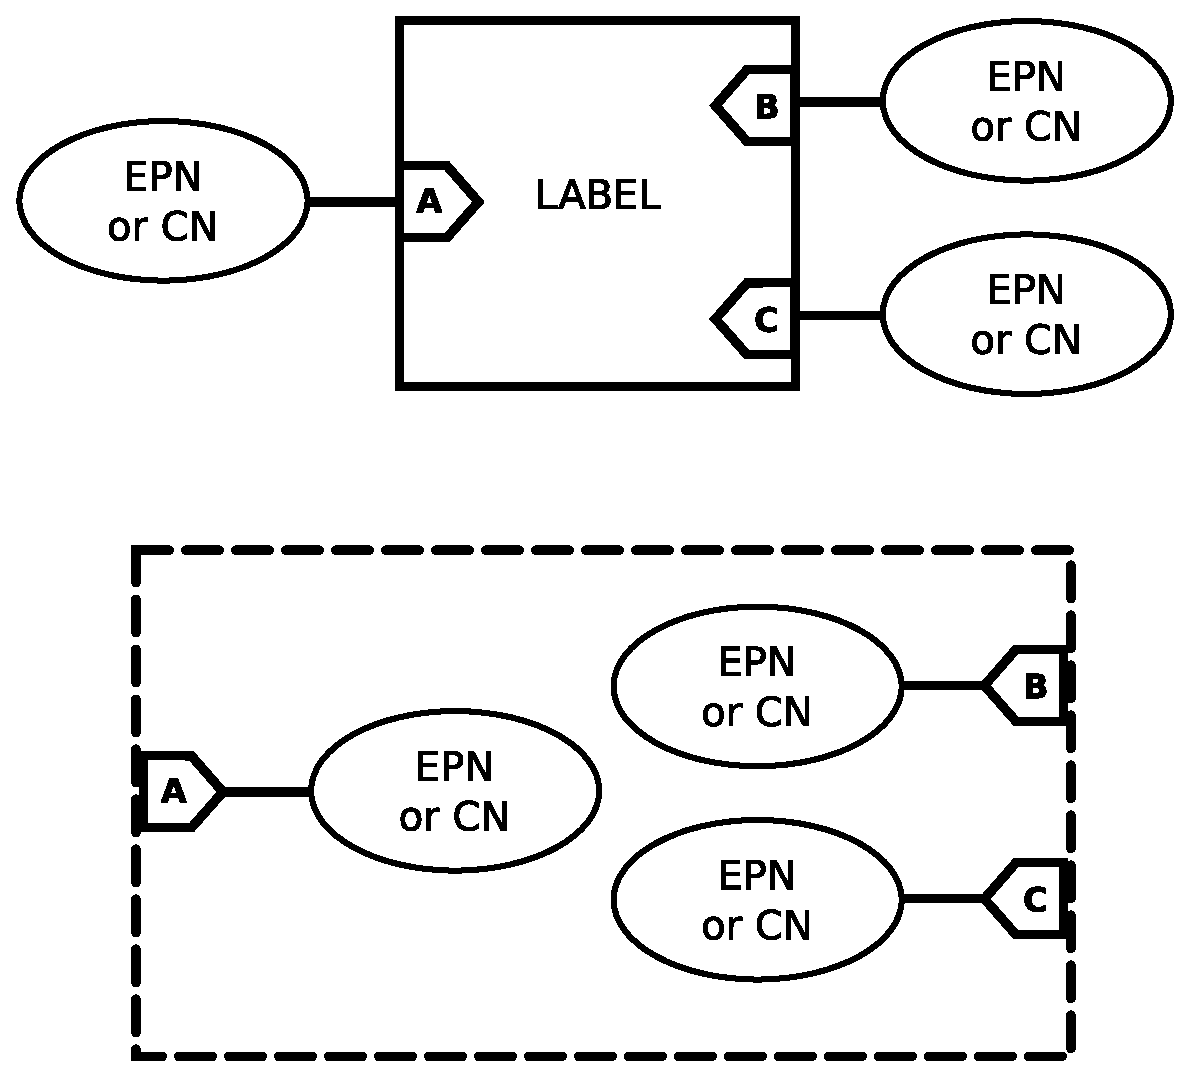
\includegraphics[scale = 0.22]{images/submap}
  \caption{The \PD glyph for \glyph{submap}. (Upper part) folded submap. (Lower part) content of the submap.}
  \label{fig:submap}
\end{figure}

\subsubsection{Changes from Previous Version}

This glyph was called \glyph{Submap} in previous version of the \PD
specification. This is confusing when talking about the Submap itself
so this glyph is now referred to as the SubmapNode to distinguish it.

\subsection{LogicalOperator}
\label{sec:logic}
\label{defn:LogicalOperator}

\begin{figure}[htb]
  \centering
  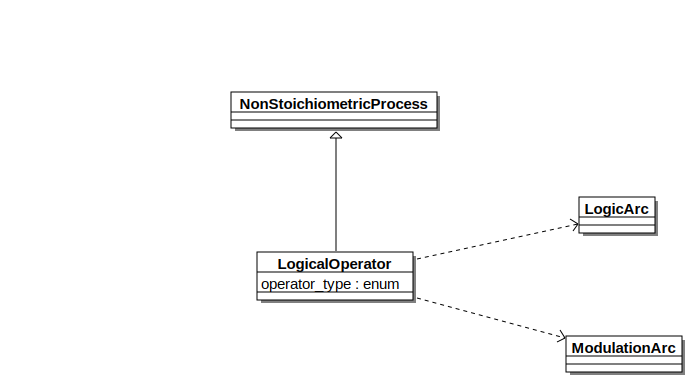
\includegraphics[width = 0.5\textwidth]{images/logicaloperatoruml}
  \caption{The UML definition of the \sbgnclass{LogicalOperator}.}
  \label{fig:logicaloperatoruml}
\end{figure}

 The \sbgnclass{LogicalOperator} (figure \ref{fig:logicaloperatoruml} performs a Boolean operation on one or
more inputs to give a binary output. The input must be a Boolean
value, and are obtained from the \classref{LogicArc} connected to the
\sbgnclass{LogicOperator}. The output a two-value quantity,  0 for False and positive
non-zero for True. This is required because the output of the
\sbgnclass{LogicOperator} must be connected to either a
\sbgnclass{LogicArc} or a \classref{ModulationArc} both of which
require their out node to provide a quality. The behaviour of the
logical operator for each type of \attrib{operator\_type} is shown in
the following table:

\begin{tabular}[t]{c p{12cm}}
\toprule
AND & All inputs must be True for output to be True, otherwise output
is false.\\
OR & At least one input must be True for output to be True. If all
inputs are False then output is False.\\
NOT & Only one input is permitted and the output is the inversion of
the input. Therefore True gives False and False gives True.\\
\bottomrule
\end{tabular}

\subsubsection{Generalisation}

\begin{itemize}
\item \classref{NonStoichiometricProcess}
\end{itemize}

\subsubsection{Attributes}

\begin{attributes}
  \attitem{operator\_type}{enum}{R} The operator type must be one of the
  following enumerations: AND, OR, NOT.
\end{attributes}

\subsubsection{Associations}

No additional associations.

\subsubsection{Rules and Constraints}

\begin{itemize}
\item \attrib{in\_arc} can only contain one or more instances of
  \sbgnclass{LogicArc}.
\item \attrib{out\_arc} can only contain one or more instances of
  \sbgnclass{LogicArc} or \sbgnclass{ModulationArc}.
\item if \attrib{operator\_type} is AND or OR, then \attrib{in\_arc} must
  contain two or more arcs.
\item if \attrib{operator\_type} is NOT then \attrib{in\_arc} must
  contain only one arc.
\item \attrib{out\_arc} can contain only one arc.
\end{itemize}

\subsubsection{Notation}

%%%%%%%%%%%%%%%%%%%%%%%%%%%%%%%%%%%%%%%%%%%%%%%%%%%%%%%%%%%%%%%%%%%%%%
%%                     And
%%%%%%%%%%%%%%%%%%%%%%%%%%%%%%%%%%%%%%%%%%%%%%%%%%%%%%%%%%%%%%%%%%%%%%
%\color{blue}
\paragraph{Glyph: \glyph{And}}\label{sec:and}

\begin{glyphDescription}
 \glyphSboTerm SBO:0000173 ! and.
 \glyphOrigin More than one \glyph{EPN} (section~\ref{sec:EPNs}) or \glyph{logical operator} (section~\ref{sec:logic}).
 \glyphTarget  One modulation (section~\ref{sec:modulation}), stimulation (section~\ref{sec:stimulation}), catalysis (section~\ref{sec:catalysis}), inhibition (section~\ref{sec:inhibition}) or necessary stimulation (section~\ref{sec:necessary_stim}) arc.
 \glyphNode \glyph{And} is represented by a circle carrying the word ``AND''.
\end{glyphDescription}

\begin{figure}[H]
  \centering
  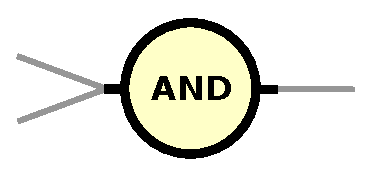
\includegraphics[scale = 0.5]{images/and}
  \caption{The \PD glyph for \glyph{and}. Only two inputs are represented, but more would be allowed.}
  \label{fig:and}
\end{figure}


%%%%%%%%%%%%%%%%%%%%%%%%%%%%%%%%%%%%%%%%%%%%%%%%%%%%%%%%%%%%%%%%%%%%%%
%%                     Or
%%%%%%%%%%%%%%%%%%%%%%%%%%%%%%%%%%%%%%%%%%%%%%%%%%%%%%%%%%%%%%%%%%%%%%
\paragraph{Glyph: \glyph{Or}}\label{sec:or}

\begin{glyphDescription}
 \glyphSboTerm SBO:0000174 ! or.
 \glyphOrigin More than one \glyph{EPN} (section~\ref{sec:EPNs}) or \glyph{logical operator} (section~\ref{sec:logic}).
 \glyphTarget  One modulation (section~\ref{sec:modulation}), stimulation (section~\ref{sec:stimulation}), catalysis (section~\ref{sec:catalysis}), inhibition (section~\ref{sec:inhibition}) or necessary stimulation (section~\ref{sec:necessary_stim}) arc.
 \glyphNode \glyph{Or} is represented by a circle carrying the word ``OR''.
 \end{glyphDescription}

\begin{figure}[H]
  \centering
  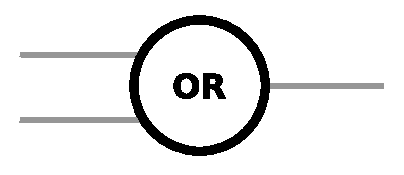
\includegraphics[scale = 0.5]{images/or}
  \caption{The \PD glyph for \glyph{or}. Only two inputs are represented, but more would be allowed.}
  \label{fig:or}
\end{figure}


%%%%%%%%%%%%%%%%%%%%%%%%%%%%%%%%%%%%%%%%%%%%%%%%%%%%%%%%%%%%%%%%%%%%%%
%%                     Not
%%%%%%%%%%%%%%%%%%%%%%%%%%%%%%%%%%%%%%%%%%%%%%%%%%%%%%%%%%%%%%%%%%%%%%
\paragraph{Glyph: \glyph{Not}}\label{sec:not}

\begin{glyphDescription}
 \glyphSboTerm SBO:0000238 ! not.
 \glyphOrigin One \glyph{EPN} (section~\ref{sec:EPNs}) or \glyph{logical operator} (section~\ref{sec:logic}).
 \glyphTarget  One modulation (section~\ref{sec:modulation}), stimulation (section~\ref{sec:stimulation}), catalysis (section~\ref{sec:catalysis}), inhibition (section~\ref{sec:inhibition}) or necessary stimulation (section~\ref{sec:necessary_stim}) arc.
 \glyphNode \glyph{Not} is represented by a circle carrying the word ``NOT''.
 \end{glyphDescription}

\begin{figure}[H]
  \centering
  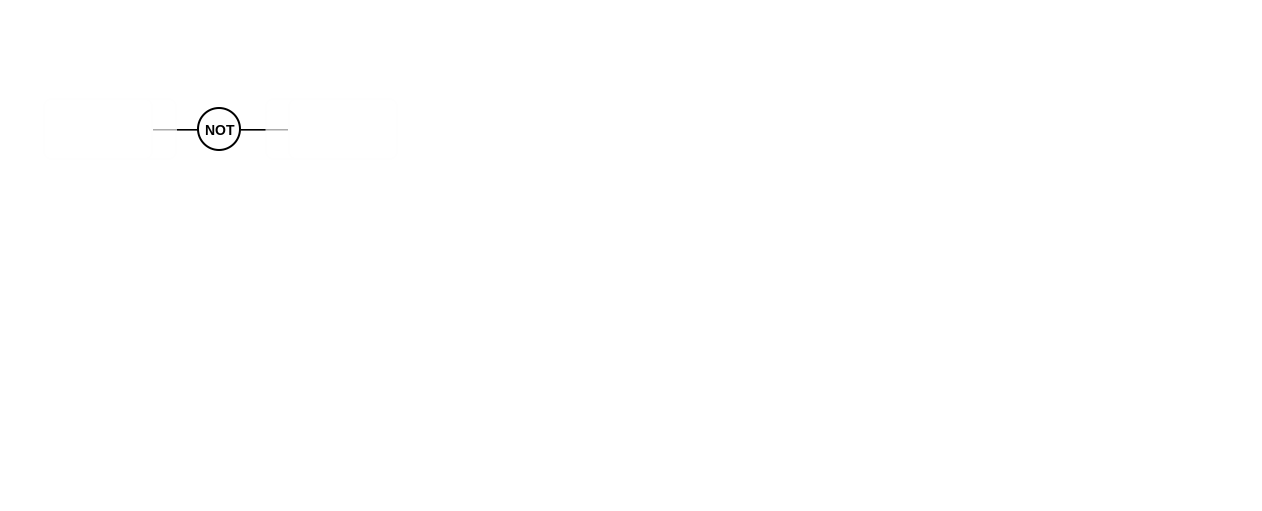
\includegraphics[scale = 0.5]{images/not}
  \caption{The \PD glyph for \glyph{not}.}
  \label{fig:not}
\end{figure}

\subsubsection{Changes from Previous Version}

Although the \sbgnclass{LogicOperator} was not explicitly defined in
the previous version the semantics and glyphs are unchanged.


\subsection{StoichiometricProcess}
\label{defn:StoichiometricProcess}\label{sec:stoichiometricprocess}

\begin{figure}[htb]
  \centering
  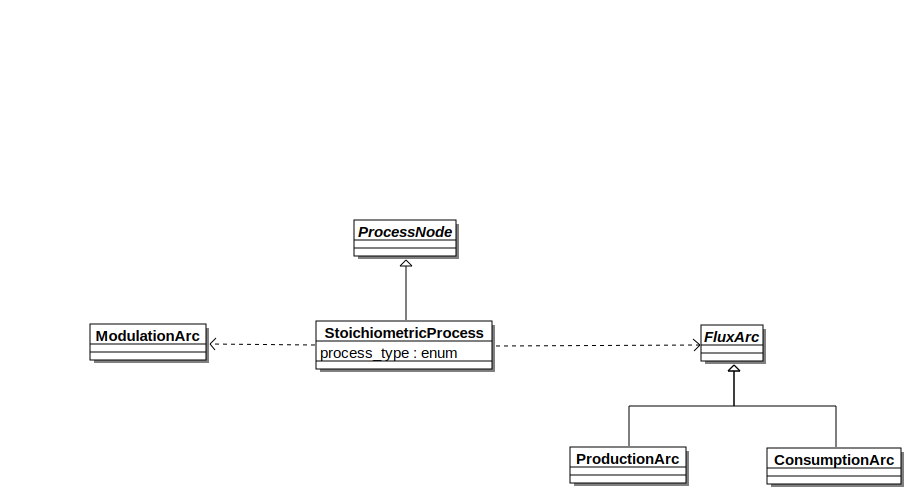
\includegraphics[width = 0.65\textwidth]{images/stoichprocessuml}
  \caption{The UML definition of the
    \sbgnclass{StiochiometricProcess}. The class interacts with
    subclasses of \sbgnclass{FluxArc} and \sbgnclass{ModulationArc}.}
  \label{fig:stoichprocessuml}
\end{figure}
 
A process that produces a measurable change in the quantities of
entity pools consumed and produced. In \PDl this is represented by the
\sbgnclass{StoichiometricProcess}. This type of process can be though
of as having a basal rate of governing the change in EPN quantities,
that is changed by other influences described by instances of
\classref{ModulationArc}. \sbgnclass{StoichiometricProcess} can be one
of several different types, which indicate the amount that is known
about the process or in some cases the nature of the process, for
example association and dissociation. The permitted values for
\attrib{process\_type} are described in the following table:

\begin{tabular}[c]{l p{12cm}}
\\\toprule
generic & A generic stoichiometric process that transforms a set of entity pools into another set of entity pools.\\
omitted & Omitted processes are processes that are known to exist, but are omitted from the map for the sake of clarity or parsimony. A single \glyph{omitted process} can represent any number of actual processes. The \glyph{omitted process} is different from a \glyph{submap}. While a \glyph{submap} references to an explicit content, that is hidden in the main map, the \glyph{omitted process} does not ``hide'' anything within the context of the map, and cannot be ``unfolded''.\\
uncertain & Uncertain processes are processes that may not exist. A single \glyph{uncertain process} can represent any number of actual processes.\\
association & The association between one or more \glyph{EPNs} represents the non-covalent binding of the biological objects represented by those \glyph{EPNs} into a larger complex.\\
dissociation & The dissociation of an \glyph{EPN} into one or more \glyph{EPNs} represents the rupture of a non-covalent binding between the biological entities represented by those \glyph{EPNs}.\\
\bottomrule\\
\end{tabular}\\


The \sbgnclass{StoichiometricProcess} describes a process that transforms a given set of biochemical entities---macromolecules, simple chemicals or unspecified entities---into another set of biochemical entities.  Such a transformation might imply modification of covalent bonds (conversion), modification of the relative position of constituents (conformational process) or movement from one compartment to another (translocation).

A cardinality label may be associated with \glyph{consumption} (\sect{consumption}) or \glyph{production} (\sect{production}) arcs to indicate the stoichiometry of the process.  This label becomes a requirement when the exact composition of the number of copies of the inputs or outputs to a reaction are ambiguous in the map.

A process is regarded as reversible if both `sides' of the process are
connected to \glyph{production} arcs (see section \ref{sec: semantics
  reversible procs}).The semantics of \glyph{modulation} is the same
as for irreversible processes, .i.e. the amount of entity in the
modulation pool affects the rate of the process.

\subsubsection{Generalisation}

\begin{itemize}
\item \classref{ProcessNode}
\end{itemize}

\subsubsection{Attributes}

\begin{attributes}
  \attitem{process\_type}{enum}{R} This must be one of the following
  enumerations: generic, omitted, uncertain, association, dissociation.
\end{attributes}

\subsubsection{Associations}

No additional associations.

\subsubsection{Rules and Constraints}

\begin{itemize}
\item The \attrib{in\_arc} must contain one or more
  \sbgnclass{FluxArc} of the same type, \ie all \sbgnclass{FluxArc}s be of class
  \sbgnclass{ConsumptionArc} or all of class
  \sbgnclass{ProductionArc}.
\item In addition the \attrib{in\_arc} may contain zero, one or more
  instances of \sbgnclass{ModulationArc}.
\item The \attrib{out\_arc} must contain one or more
 instances of \sbgnclass{ProductionArc}.
\item If \attrib{process\_type} is association then the
  \attrib{in\_arc} must only contain arcs of type
  \sbgnclass{ConsumptionArc} and \attrib{out\_arc} can only contain
  one \sbgnclass{ProductionArc}.
\item If \attrib{process\_type} is dissociation then the
  \attrib{in\_arc} can contain only one \sbgnclass{ConsumptionArc}
  instance.
\item If a \sbgnclass{StoichiometricProcess} only contains in and out
  arcs of class \sbgnclass{ProductionArc} then it is regarded as
  reversible.
\end{itemize}

\subsubsection{Notation}

\paragraph{Glyph: \glyph{Process}}
\label{sec:process}

\begin{glyphDescription}

\glyphSboTerm SBO:0000375 ! process

\glyphOrigin One or several \glyph{consumption} arcs (\sect{consumption}) or one or several \glyph{production} arcs (\sect{production}).

\glyphTarget One or several \glyph{production} arcs (\sect{production}).

\glyphNode A process is represented by a square box linked to two
connectors, small arcs attached to the centers of opposite sides. The
consumption (\sect{consumption}) and production (\sect{production})
arcs are linked to the extremities of those connectors. The modulatory
arcs (section \ref{sec:modulation}) point to the other two sides of the box. A \glyph{process} connected to \glyph{production} arcs on opposite sides is a reversible process. 

\end{glyphDescription}

\begin{figure}[H]
  \centering
  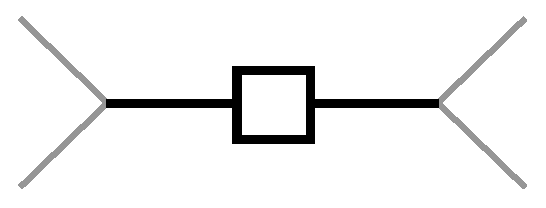
\includegraphics[scale = 0.4]{images/process}
  \caption{The \PD glyph for \glyph{process}.}
  \label{fig:process}
\end{figure}


The example in \fig{trans-phos} illustrates the use of a \glyph{process} node to represent the phosphorylation of a protein in a \PD.

\begin{figure}[H]
  \centering
  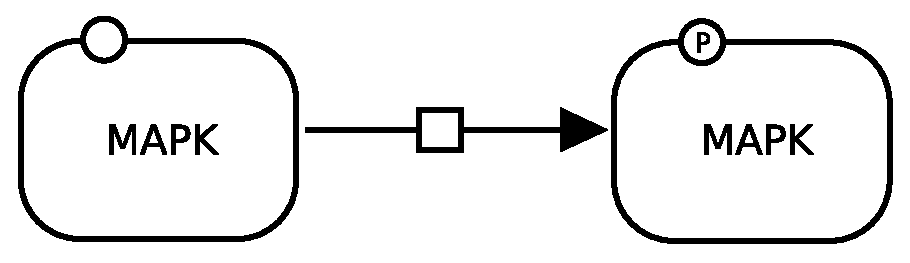
\includegraphics[scale = 0.3]{examples/process-phosphorylation}
  \caption{Phosphorylation of the protein MAP kinase.}
  \label{fig:trans-phos}
\end{figure}

The example in \fig{trans-react} illustrates the use of a \glyph{process} node to represent a reaction between two reactants that generates three products. 

\begin{figure}[H]
  \centering
  \includegraphics[scale = 0.3]{examples/process-reaction}
  \caption{Reaction between ATP and fructose-6-phosphate to produce fructose-1,6-biphosphate, ADP and a proton.}
  \label{fig:trans-react}
\end{figure}

The example in \fig{trans-trans} illustrates the use of a \glyph{process} node to represent a translocation. The large round-cornered rectangle represents a compartment border (see \sect{compartment}).

\begin{figure}[H]
  \centering
  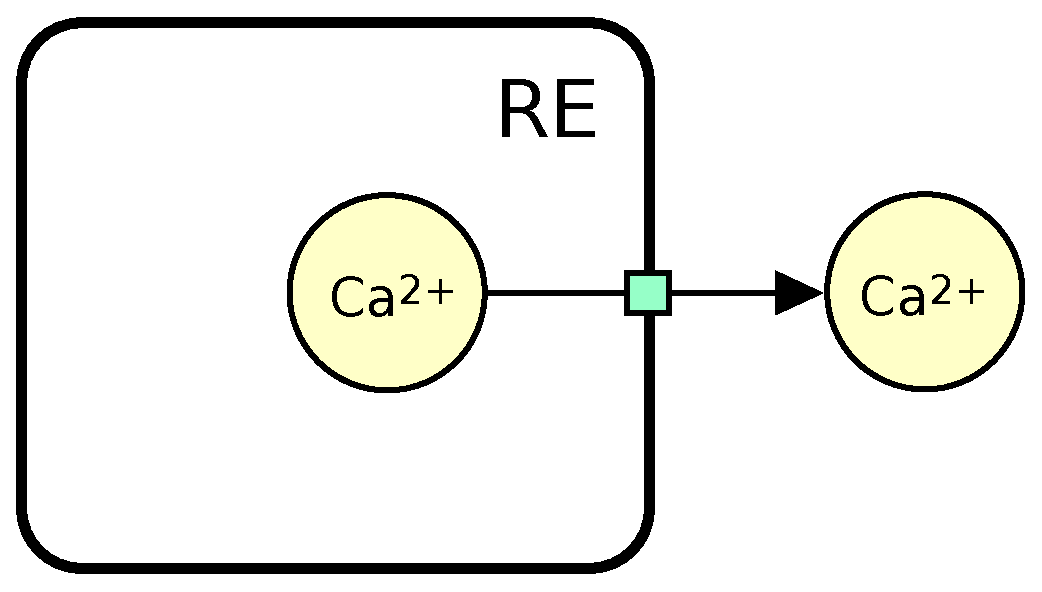
\includegraphics[scale = 0.3]{examples/process-translocation}
  \caption{Translocation of calcium ion out of the endoplasmic reticulum. Note that the \glyph{process} does not have to be located on the boundary of the \glyph{compartment}. A \glyph{process} is not attached to any \glyph{compartment}.}
  \label{fig:trans-trans}
\end{figure}

The example in \fig{trans-reverse} illustrates the use of a \glyph{process} node to represent the reversible opening and closing of an ionic channel in a \PD.

\begin{figure}[H]
  \centering
  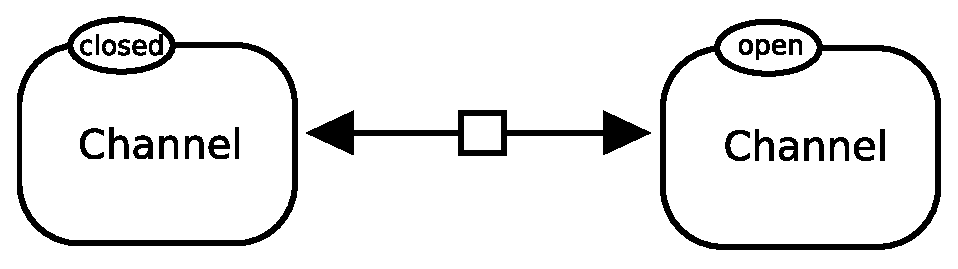
\includegraphics[scale = 0.3]{examples/process-reversible}
  \caption{Reversible opening and closing of an ionic channel.}
  \label{fig:trans-reverse}
\end{figure}

When such a reversible process is asymmetrically modulated, it must be represented by two different processes in a \PD.  \fig{trans-mod} illustrates the use of two \glyph{process} nodes to represent the reversible activation of a G-protein coupled receptor.  In the absence of any effector, an equilibrium exists between the inactive and active forms.  The agonist stabilises the active form, while the inverse agonist stabilises the inactive form.

\begin{figure}[H]
  \centering
  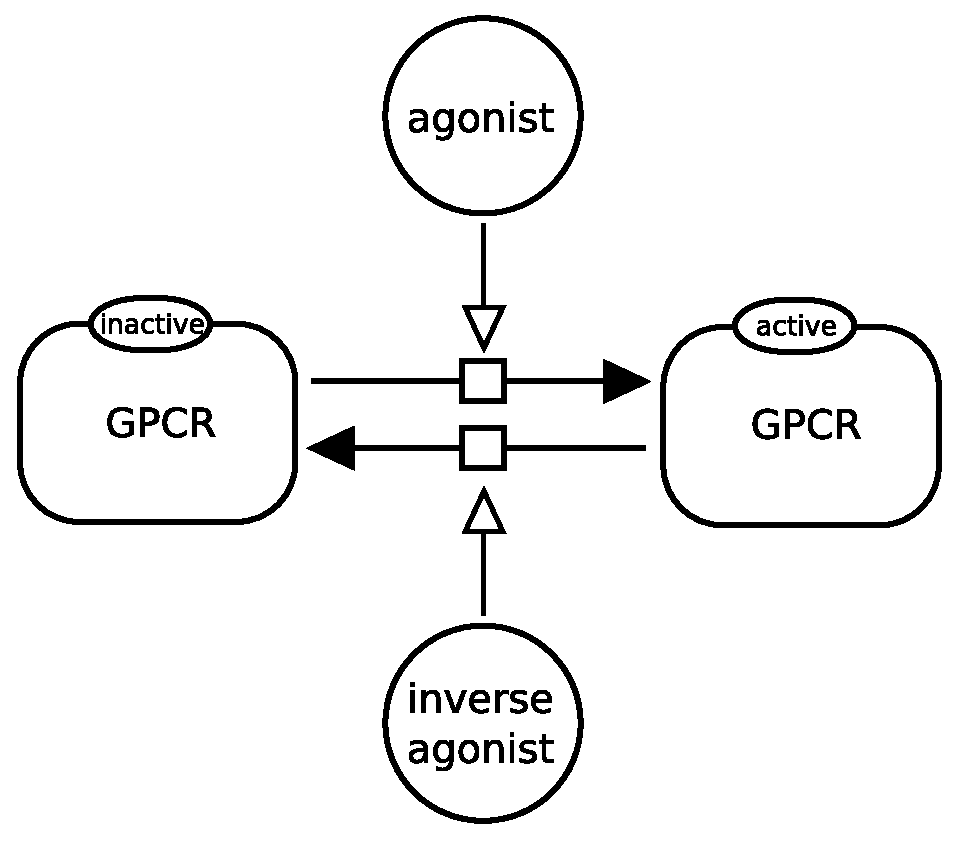
\includegraphics[scale = 0.3]{examples/process-modulated}
  \caption{The reversible activation of a G-protein coupled receptor.}
  \label{fig:trans-mod}
\end{figure}

The example in \fig{trans-dim} presents the conversion of two galactoses into a lactose.  Galactoses are represented by only one \glyph{simple chemical}, the cardinality being carried by the \glyph{consumption} arc.

\begin{figure}[H]
  \centering
  
\includegraphics[scale = 0.3]{examples/process-dimerisation}
  \caption{Conversion of two galactoses into a lactose.}
  \label{fig:trans-dim}
\end{figure}


%%%%%%%%%%%%%%%%%%%%%%%%%%%%%%%%%%%%%%%%%%%%%%%%%%%%%%%%%%%%%%%%%%%%%%
%%                     Omitted Process
%%%%%%%%%%%%%%%%%%%%%%%%%%%%%%%%%%%%%%%%%%%%%%%%%%%%%%%%%%%%%%%%%%%%%%

\paragraph{Glyph: \glyph{Omitted process}}\label{sec:omitted}


\begin{glyphDescription}
 \glyphSboTerm SBO:0000397 - omitted process.
 \glyphOrigin One or several \glyph{consumption} arcs (\sect{consumption}) or one or several \glyph{production} arcs (\sect{production}).
 \glyphTarget One or several \glyph{production} arcs (\sect{production}).

 \glyphNode An \glyph{omitted process} is represented by a \glyph{process} in which the square box contains a two parallel slanted lines oriented northwest-to-southeast and separated by an empty space.
 \end{glyphDescription}

\begin{figure}[H]
  \centering
  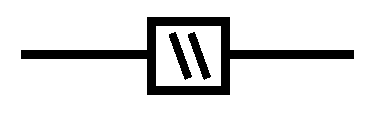
\includegraphics[scale = 0.5]{images/omitted}
  \caption{The \PD glyph for \glyph{omitted process}.}
  \label{fig:omitted}
\end{figure}


%%%%%%%%%%%%%%%%%%%%%%%%%%%%%%%%%%%%%%%%%%%%%%%%%%%%%%%%%%%%%%%%%%%%%%
%%                     Uncertain Process
%%%%%%%%%%%%%%%%%%%%%%%%%%%%%%%%%%%%%%%%%%%%%%%%%%%%%%%%%%%%%%%%%%%%%%

\paragraph{Glyph: \glyph{Uncertain process}}\label{sec:uncertain}

\begin{glyphDescription}
 \glyphSboTerm SBO:0000396 ! uncertain process.
 \glyphOrigin One or several \glyph{consumption} arcs (\sect{consumption}) or one or several \glyph{production} arcs (\sect{production}).
 \glyphTarget One or several \glyph{production} arcs (\sect{production}).
 \glyphNode An \glyph{uncertain process} is represented by a \glyph{process} which square box contains a question mark.
 \end{glyphDescription}

\begin{figure}[H]
  \centering
  \includegraphics[scale = 0.5]{images/uncertain}
  \caption{The \PD glyph for an \glyph{uncertain process}.}
  \label{fig:uncertain}
\end{figure}


%%%%%%%%%%%%%%%%%%%%%%%%%%%%%%%%%%%%%%%%%%%%%%%%%%%%%%%%%%%%%%%%%%%%%%
%%                     Association
%%%%%%%%%%%%%%%%%%%%%%%%%%%%%%%%%%%%%%%%%%%%%%%%%%%%%%%%%%%%%%%%%%%%%%

\paragraph{Glyph: \glyph{Association}}\label{sec:association}


\begin{glyphDescription}
 \glyphSboTerm SBO:0000177 ! non-covalent binding.
 \glyphOrigin One or more \glyph{consumption} arcs (\sect{consumption}).
 \glyphTarget  One \glyph{production} arc (\sect{production}).
 \glyphNode An \glyph{association} between several entities is represented by a filled disc linked to two connectors, small arcs attached on point separated by 180 degrees. The consumption (\sect{consumption}) and production (\sect{production}) arcs are linked to the extremities of those connectors. 
 \end{glyphDescription}

\begin{figure}[H]
  \centering
  
\includegraphics[scale = 0.5]{images/association}
  \caption{The \PD glyph for \glyph{association}.}
  \label{fig:association}
\end{figure}

The example in \fig{assoc-cyclin} illustrates the association of cyclin and CDC2 kinase into the Maturation Promoting Factor.

\begin{figure}[H]
  \centering
  \includegraphics[scale = 0.3]{examples/association-MPF}
  \caption{Association of cyclin and CDC2 kinase into the Maturation Promoting Factor.}
  \label{fig:assoc-cyclin}
\end{figure}

\fig{assoc-unamed} gives an example illustrating the association of a pentameric macromolecule (a nicotinic acetylcholine receptor) with a simple chemical (the local anesthetic chlorpromazin) in an unnamed complex.

\begin{figure}[H]
  \centering
  \includegraphics[scale = 0.3]{examples/association-unamed}
  \caption{The association of a pentameric macromolecule with a simple chemical in an unnamed complex.}
  \label{fig:assoc-unamed}
\end{figure}

An association does not necessarily result in the formation of a \glyph{complex}; it can also produce a \glyph{multimer}, or a \glyph{macromolecule} (although the latter case is semantically borderline).  \ref{fig:assoc-multi} gives an example of this, using the formation of hemoglobin.

\begin{figure}[H]
  \centering
  \includegraphics[scale = 0.3]{examples/association-multimerisation}
  \caption{Formation of hemoglobin.}
  \label{fig:assoc-multi}
\end{figure}

\paragraph{Glyph: \glyph{Dissociation}}\label{sec:dissociation}

\begin{glyphDescription}
 \glyphSboTerm SBO:0000180 ! dissociation.
 \glyphOrigin One \glyph{consumption} arc (\sect{consumption}).
 \glyphTarget  One or more \glyph{production} arc (\sect{production}).
 \glyphNode A \glyph{dissociation} between several entities is represented by two concentric circles. A simple empty disc could be, in some cases, confused with the \glyph{catalysis} (section \sect{catalysis}). Moreover, the existence of two circles reminds the dissociation, by contrast with the filled disc of the \glyph{association} (\sect{association}).
 \end{glyphDescription}


\begin{figure}[H]
  \centering
  \includegraphics[scale = 0.5]{images/dissociation}
  \caption{The \PD glyph for \glyph{dissociation}.}
  \label{fig:dissociation}
\end{figure}

The example in \fig{dissoc-ribo} illustrates the dissociation of the small and large ribosomal subunits from a messenger RNA.

\begin{figure}[H]
  \centering
  \includegraphics[scale = 0.3]{examples/dissociation-ribosome}
  \caption{Dissociation of the small and large ribosomal subunits from a messenger RNA.}
  \label{fig:dissoc-ribo}
\end{figure}

\subsubsection{Changes from Previous Version}

Although the \sbgnclass{NonStoichiometricProcess} was not explicitly defined in
the previous version the semantics and glyphs are unchanged.
 
\subsection{Compartment}
\label{defn:Compartment}

\begin{figure}[htb]
  \centering
  \includegraphics[width = 0.5\textwidth]{images/compartmentuml}
  \caption{The UML definition of the \sbgnclass{Compartment} showing
    how it containment of \sbgnclass{EntityPoolNode}.}
  \label{fig:compartmentuml}
\end{figure}

The \sbgnclass{Compartment} is a logical or physical structure that
contains entity pool nodes. An \classref{EntityPoolNode} can only
belong to one compartment. Therefore, the ``same'' biochemical species
located in two different compartments are in fact two different pools.


\subsubsection{Generalisation}

\begin{itemize}
\item \classref{SBGNGlyph}
\end{itemize}

\subsubsection{Attributes}

\begin{attributes}
  \attitem{name}{string}{R} The name of the compartment.
  \attitem{natures}{cv}{*} A set of controlled vocabularies that describes
  a characteristic of the compartment. Zero, one or more values may be
  set, but each one must belong to a different controlled vocabulary.
\end{attributes}

\subsubsection{Associations}

\begin{attributes}
  \associtem{epns}{EntityPoolNode}{*} The
  \sbgnclass{EntityPoolNode}s contained by this compartment.
\end{attributes}

\subsubsection{Rules and Constraints}

\begin{itemize}
\item \attrib{name} must not be used by another instance of
  \sbgnclass{Container} contained by the same instance of
  \sbgnclass{Map}.
\item \attrib{epns} must contain a unique set of
  \sbgnclass{EntityPoolNodes}. See section \ref{sec:epnuniqueness} for
  the definition of \sbgnclass{EntityPoolNode} uniqueness.
\end{itemize}

\subsubsection{Notation}

\paragraph{Glyph: \glyph{Compartment}}\label{sec:compartment}

\begin{glyphDescription}

\glyphSboTerm  SBO:0000290 ! physical compartment 

\glyphContainer A compartment is represented by a surface enclosed in a continuous border or located between continuous borders. These borders should be noticeably thicker than the borders of the EPNs. A compartment can take \textbf{any} geometry. A compartment must always be entirely enclosed.

\glyphLabel The identification of the compartment is carried by an unbordered box containing a string of characters. The characters can be distributed on several lines to improve readability, although this is not mandatory. The label box can be attached anywhere in the container box. Note that the label can spill-over from the container box.

\glyphAux A \glyph{compartment} can carry a certain number of \glyph{units of information}, that will add information for instance about the physical environment, such as pH, temperature or voltage, see \sect{unitInfo}.  The center of the bounding box of a \glyph{unit of information} is located on the mid-line of the border of the compartment.

\end{glyphDescription}

\begin{figure}[H]
  \centering
  \includegraphics[scale = 0.3]{images/compartment}
  \caption{The \PD glyph for \glyph{compartment}.}
  \label{fig:compartment}
\end{figure}


To allow more aesthetically pleasing and understandable maps, compartments are allowed to overlap each other visually, but it must be kept in mind that this does not mean the top compartment contains part of the bottom compartment.  \fig{overlap} shows two semantically equivalent placement of compartments:

\begin{figure}[H]
  \centering
  \includegraphics[scale = 0.4]{examples/compartment_overlapping}
  \caption{Overlapped compartments are permitted, but the overlap does not imply containment.}
  \label{fig:overlap}
\end{figure}

Overlapped (hidden) part of the compartment should not contain any object which could be covered by an overlapping compartment.  \fig{overlap-bad} illustrates the problem using an incorrect map.

\begin{figure}[H]
  \centering
  \includegraphics[scale = 0.45]{examples/compartment_overlapping_wrong}
  \caption{Example of an \textbf{incorrect} map.  Overlapped compartments must not obscure other objects.}
  \label{fig:overlap-bad}
\end{figure}

% It is important to note that a compartment never contains another compartment, but may surround it.  A key aspect of correctly drawing two ``adjacent'' compartments is that they are not separated by one line, but by \textbf{two} lines.  \fig{two-comp} provides an example of this in which a cell is shown made up of a nucleus surrounded by the cytoplasm.

% \begin{figure}[H]
%   \centering
%   \includegraphics[scale = 0.4]{examples/compartment-cell}
%  \includegraphics[scale = 0.4]{examples/compartment-cell-wrong}
%   \caption{Compartments can surround other compartments; in that case, both of the compartment's borders must still be shown, with the result that the separation is drawn as two lines. The left example is correct, with twoo disjoint compartments representing the ``cytoplasm'' and the ``nucleus''. The right example is incorrect. Indeed the compartments ``cell'' and ``nucleus'' would be disjoint, the latter only overlapping the former. As a result, the volume of the nucleus is duplicated.}
%   \label{fig:two-comp}
% \end{figure}

% The example diagram in \fig{three-comp} represents three adjacent compartments.  Two of the compartments carry units of information.  Notice that these units of information do not overlap multiple membrane boundaries.

% \begin{figure}[H]
%   \centering
%   \includegraphics[scale = 0.4]{examples/compartment-3comp}
%   \caption{Illustration of units of information and surrounding compartments.}
%   \label{fig:three-comp}
% \end{figure}

\subsubsection{Changes from Previous Version}

No changes from previous the version.

\subsection{AttributeValue}
\label{defn:AttributeValue}

\begin{figure}[htb]
  \centering
  \includegraphics[width = 0.5\textwidth]{images/attributevalueuml}
  \caption{The UML definition of the \sbgnclass{AttributeValue} and
    its usage by other classes.}
  \label{fig:attributevalueuml}
\end{figure}

 The \sbgnclass{AttributeValue} is used to present the values of
 certain attributes held by other SBGN elements. It is typically
 contained and owned by the class containing the attribute (or its
 descendants). It contains two values, one is a \attrib{code} to indicate the
 attribute that is defined and the other is the\attrib{ value} itself. The \attrib{code}
 and the presentation format of the \attrib{value} are defined by the
 SBGN element that contains the \sbgnclass{AttributeValue}, currently
 \classref{Compartment}, \classref{EntityPoolNode}, and \classref{Subunit}.


\subsubsection{Generalisation}

\begin{itemize}
\item \classref{AuxiliaryUnit}
\end{itemize}

\subsubsection{Attributes}

\begin{attributes}
  \attitem{code}{string}{R} The code indicating the attribute that is
  being presented.
  \attitem{value}{object}{R} The value of the attribute. The format of
  the value is determined by the class holding the attribute.
\end{attributes}

\subsubsection{Associations}

No additional associations.

\subsubsection{Rules and Constraints}

No additional rules and constraints.

\subsubsection{Notation}

For historical reasons the \sbgnclass{AttributeValue} is represented
graphically by the glyph \glyph{Unit of Information}.

\paragraph{Glyph: \glyph{Unit of information}}
\label{sec:unitInfo}

When representing biological entities, it is often necessary to convey
some abstract information about the entity's function that cannot (or
does not need to) be easily related to its structure.  The \glyph{unit
  of information} is a decoration that can be used in this situation
to add information to a glyph.  Some example uses include:
characterizing a logical part of an entity such as a functional domain
(a binding domain, a catalytic site, a promoter, etc.), or the
information encoded in the entity (an exon, an open reading frame,
etc.).  A \glyph{unit of information} can also convey information
about the physical environment, or the specific type of biological
entity it is decorating.

\begin{glyphDescription}

\glyphSboTerm Not applicable.

\glyphContainer A unit of information is represented by a rectangle.  The long side of the rectangle should be oriented parallel to the border of the \glyph{EPN} being annotated by the \glyph{unit of information}. The center of the bounding box of a \glyph{state of information} should be located on the mid-line of the border of the \glyph{EPN}.

\glyphLabel A \glyph{unit of information} is identified by a label placed in an unbordered box containing a string of characters.  The characters can be distributed on several lines to improve readability, although this is not mandatory.  The label box must be attached to the center of the container.  The label may spill outside of the container.


%\glyphAux A \glyph{unit of information} does not carry any auxiliary items.  

\end{glyphDescription}

\begin{figure}[H]
  \centering
  \includegraphics[scale = 0.3]{images/unitInformation}
  \caption{The \PD glyph for \glyph{unit of information}.}
  \label{fig:unitInfo}
\end{figure}


\subsubsection{Changes from Previous Version}

There was no definition of the \sbgnclass{AttributeValue} in the
previous version of this specification. However, the \glyph{Unit of
  Information} did exist although its semantics have been changed. It
no longer can hold arbitrary annotation but must display an attribute
value and observe the constraints set out by the definition of the
class owning the attribute.

Since the use of the \glyph{Unit of Information} has been deprecated,
it is recommended that \classref{Annotation} and the
\glyph{Annotation} glyph is used instead.

\subsection{StateVariable}
\label{defn:StateVariable}

Many biological entities such as molecules can exist in different
\emph{states}, meaning different physical or informational
configurations.  These states can arise for a variety of reasons.  For
example, macromolecules can be subject to post-synthesis
modifications, wherein residues of the macromolecules (amino acids,
nucleosides, or glucid residues) are modified through covalent linkage
to other chemicals.  Other examples of states are alternative
conformations as in the closed/open/desensitized conformations of a
transmembrane channel, and the active/inactive forms of an enzyme.

SBGN provides a means of associating one or more
\sbgnclass{StateVariable} with an entity (figure
\ref{fig:statevariableviewuml}); each such variable can be used to
represent a dimension along which the state of the overall entity can
vary.  When an entity can exist in different states, the state of the
whole entity (\ie the SBGN object) can be described by the set of
\sbgnclass{StateVariable} instances it contains. Note that this is
true for the \classref{Complex} where any state variables are
associated visually with subunits (c.f \classref{Subunit}), but
actually belong to the complex (figure
\ref{fig:statevariableviewuml}).

\begin{figure}[htb]
  \centering
  \includegraphics[width = 0.5\textwidth]{images/statevariableviewuml}
  \caption{The UML definition of the \sbgnclass{StateVariable} showing
    its relationship to \sbgnclass{StatefulEPN}, \sbgnclass{Complex}
    and \sbgnclass{Subunit}.}
  \label{fig:statevariableviewuml}
\end{figure}

\subsubsection{Generalisation}

\begin{itemize}
\item \classref{AuxiliaryUnit}
\end{itemize}

\subsubsection{Attributes}

\begin{attributes}
  \attitem{name}{string}{O} The name of the state variable. This value is
  optional.
  \attitem{value}{string}{R} The value of the state variable. This is
  optional, but cannot be an empty string.
\end{attributes}

\subsubsection{Associations}

\begin{attributes}
  \associtem{owning\_epn}{StatefulEPN}{1}  The stateful EPN that owns
  the state variable.
\end{attributes}

\subsubsection{Rules and Constraints}

\begin{itemize}
\item The symbols in the 
\end{itemize}

\subsubsection{Notation}


\paragraph{Glyph: \glyph{State variable}}
\label{sec:stateVariable}


\begin{glyphDescription}

\glyphSboTerm Not applicable.

\glyphContainer A \glyph{state variable} is represented by a
``stadium'' container, that is two hemicercles of same radius joined
by parallel segments, as shown in \fig{state-var}.  The parallel
segment axis should be tangent to the border of the glyph of the
\glyph{EPN} being modified by the \glyph{state variable}. The center
of the bounding box of a \glyph{state variable} should be located on
the mid-line of the border of the \glyph{EPN}. In previous versions of
this specification the \glyph{state variable} was represented by an
ellipse. This symbols is now \textbf{deprecated} in favour of the stadium
symbol described above. New \PD maps should not use the ellipse symbol.

\glyphLabel An unbordered box containing a string indicating the
contents of the \sbgnclass{StateVariable}. The style of labeling of
\glyph{State Variables} encouraged by \SBGNPDLone is to combine a
prefix representing the value of the variable with a suffix
representing the variable's name.  Prefix and suffix should be
separated by the symbol '@', X@Y thus meaning \emph{value X} AT
\emph{variable Y}. If \attrib{name} is undefined then only the value
should be displayed and the '@' character omitted.  If both the
\attrib{name} and \attrib{value} are undefined then the label should
be empty (\ie an empty string). The label of a \glyph{state variable}
should, if possible, be displayed within the boundary of the glyph. In
earlier versions of the SBGN specification it was permitted to
separate the \attrib{name} and \attrib{value} into two unlabelled
boxes and display the \attrib{name} box outside the \glyph{state
  variable} glyph. This is now \textbf{deprecated} and new \PD maps
should not use this notation.


% The identification of an instance of a \glyph{state variable} is carried by one or two unbordered boxes, each containing a string of characters.  The characters cannot be distributed on several lines.  One box is mandatory, and contains the value of the \glyph{state variable}.  The value may be empty; an example of a situation where this might arise is an unphosphorylated phosporylation site.  The second box is optional and carries the identification of the \glyph{state variable}. The center of the combination of the boxes located in the container box is superposed to the center of this container box.  In earier version of the \PD specification, the identification of the \glyph{state variable} could be located outside the \glyph{state variable} container box.  This is now forbidden.  The style of labeling of \glyph{state variables} encouraged by \SBGNPDLone is to combine a prefix representing the value of the variable with a suffix representing the variable's name.  Prefix and suffix should be separated by the symbol '@', X@Y thus meaning \emph{value X} AT \emph{variable Y}. The label of a \glyph{state variable} should, if possible, be displayed within the boundary of the glyph.

\glyphAux A \glyph{state variable} does not carry any auxiliary items.  

\end{glyphDescription}

\begin{figure}[H]
  \centering
  \includegraphics[scale = 0.3, trim = 0 0 0 0.25in]{images/stateVariable}
  \caption{Examples of the \PD glyph for \glyph{state variable}.}
  \label{fig:state-var}
\end{figure}

A \glyph{state variable} does not necessarily have to be
Boolean-valued.  For example, an ion channel can possess several
conductance states; a receptor can be inactive, active and
desensitized; and so on.  As another example, a \glyph{state variable}
``ubiquitin'' could also carry numerical values corresponding to the
number of ubiquitin molecules present in the tail.  However, in all
cases, a \glyph{state variable} on an EPN can only take \emph{one}
defined value.  Further, an EPN's \glyph{state variable} should always
be displayed and always set to a value.  An ``empty'' \glyph{state
  variable} is a \glyph{state variable} that is set to the value
``unset'', it is not a \glyph{state variable} with no value. Note that
the value ``unset'' is \emph{not} synonymous to ``any value'' or
``unknown value''.


\subsubsection{Changes from Previous Version}

The \sbgnclass{StateVariable} class was not explicitly defined in
previous versions of the specification, however the \glyph{state
  variable} was. Some aspects of its notation have been deprecated and
these are detailed above (section \ref{sec:stateVariable}).

\subsection{Annotation}
\label{defn:Annotation}

In \SBGNPDLone there are cases where the language does not capture
everything the author wishes to convey. This may be additional
experimental detail or descriptions of mechanisms that cannot be
described full by the \PDl. In this case the language provides the
\sbgnclass{Annotation}. This contains text and is associated with a
particular glyph in a map. Importantly, it is purely ``decoration''
and does alter the meaning the map.


\subsubsection{Generalisation}

\begin{itemize}
\item \classref{AuxiliaryUnit}
\end{itemize}

\subsubsection{Attributes}

\begin{attributes}
  \attitem{annotation\_text}{string}{R} The text of the
  annotation. The text is mandatory and cannot be empty or just
  spaces.
\end{attributes}

\subsubsection{Associations}

\begin{attributes}
  \associtem{annotated\_glyph}{SBGNGlyph}{1} The instance
  of \sbgnclass{SBGNGlyph} that is being annotated\footnote{Note that
    as a result of this association only glyphs and \textbf{not}
    auxiliary items may be annotated by instances of
    \sbgnclass{Annotation}}.
\end{attributes}

\subsubsection{Rules and Constraints}

No additional rules and constraints.

%\begin{itemize}
%\item
%\end{itemize}

\subsubsection{Notation}

\paragraph{Glyph: \glyph{Annotation}}

\begin{glyphDescription}

\glyphSboTerm SBO:NEW

\glyphContainer An \glyph{annotation} is represented by a rectangular
container with a folded corner, as illustrated in
\fig{annotation}. This container is linked to the annotated element
via a callout (see figure \ref{fig:ex-annotation}. The callout should
overlap with the object it is annotating.

\glyphLabel An \glyph{annotation} contains information placed in an unbordered box containing a string of characters.  The characters can be distributed on several lines to improve readability, although this is not mandatory.  The label box must be attached to the center of the container. The label may spill outside of the container. 

\glyphAux An \glyph{annotation} does not carry any auxiliary unit.
\end{glyphDescription}

\begin{figure}[H]
  \centering
  \includegraphics[scale = 0.3]{images/annotation}
  \caption{The \PD glyph for \glyph{annotation}.}
  \label{fig:annotation}
\end{figure}

\begin{figure}[H]
  \centering
  \includegraphics[scale = 0.5]{examples/ex-annotation}
  \caption{Example of \glyph{annotations} adding information to the description of the trans-phosphorylation of CaMKII. Note that three different types of links are used between annotation nodes and annotated elements. However, it is recommended to use a consistent scheme whithin a map.}
  \label{fig:ex-annotation}
\end{figure}

\subsubsection{Changes from Previous Version}

This is a new language element and an not previous versions of the \PDl.


\subsection{CrossReference}
\label{defn:CrossReference}

\begin{figure}[htb]
  \centering
  \includegraphics[width = 0.5\textwidth]{images/crossreferenceuml}
  \caption{The UML definition of the \sbgnclass{Crossreference} showing
    its subclasses \sbgnclass{Tag} and \sbgnclass{SubmapTerminal} and
    its association with other elements in the \PDl.}
  \label{fig:crossreferenceuml}
\end{figure}


\sbgnclass{CrossReference} handles links or relationships between elements of a
map and su-map. At present there is only one reference glyph,
\glyph{tag}, which can be used in a map refered to by a \glyph{submap}
(\sect{submap}) or as an auxilary unit on the \glyph{submap}. The
\glyph{clone marker} can also provide additional reference mechanisms
and is discussed below (\sect{cloneMarker}).

\subsubsection{Generalisation}

None

\subsubsection{Attributes}

\begin{attributes}
  \attitem{reference\_id}{string}{R} a string that identifies the
  cross-reference. The string cannot start and end in white space and
  cannot be empty.
\end{attributes}

\subsubsection{Associations}

\begin{attributes}
  \associtem{equivalence}{EquivalenceArc}{1} The
  equivalence arc that links this class to the referenced element.
\end{attributes}

\subsubsection{Rules and Constraints}

\begin{itemize}
\item  Two or more instances of \sbgnclass{CrossReference} with the
  same \attrib{reference\_id} value are pointing to the same element.
\item The above rules applies within a \PDm's namespace (see section \ref{sec:mapsubmaps}).
\end{itemize}

\subsubsection{Changes from Previous Version}

Not defined in the previous version.

 \subsection{SubmapTerminal}
\label{defn:SubmapTerminal}

A \sbgnclass{SubmapTerminal} (figure \ref{fig:submapnodeuml}) is a named reference that is part of a
\classref{SubmapNode}. It provides the reference that is the link to a
tag in the submap that the \sbgnclass{SubmapNode} refers to.

\subsubsection{Generalisation}

\begin{itemize}
\item \classref{AuxiliaryUnit}
\item \classref{CrossReference}
\end{itemize}

\subsubsection{Attributes}

No additional attributes.

\subsubsection{Associations}

No additional associations.

\subsubsection{Rules and Constraints}

No additional rules and constraints.

\subsubsection{Notation}

\paragraph{Glyph: \glyph{Submap Terminal}}

\begin{glyphDescription}

\glyphSboTerm Not applicable.

\glyphContainer A \glyph{tag} is represented by a rectangle fused to
an empty arrowhead.  The
flat edge opposite the arrowhead should be aligned to the edge of the
\glyph{Submap} glyph and the connecting should connect to the middle
of this face (see figure \ref{fig:submapterminal}). 

\glyphLabel A \glyph{tag} is identified by a label placed in an
unbordered box containing a string of characters.  The characters can
be distributed on several lines to improve readability, although this
is not mandatory.  The label box must be attached to the center of the
container. The label may spill outside of the container.

\glyphAux A \glyph{tag} does not carry any auxiliary items. 

\end{glyphDescription}

\begin{figure}[H]
  \centering
  \includegraphics[scale = 0.3]{images/submapterminal}
  \caption{The \PD glyph for \glyph{Submap Terminal}. This shows the
    basic glyph and its correct usage within a \glyph{Submap} glyph.}
  \label{fig:submapterminal}
\end{figure}

\subsubsection{Changes from Previous Version}

Clarified that the tag does not link a \sbgnclass{Compartment}, but
only instances of \sbgnclass{EntityPoolNode}.

\subsection{Tag}
\label{defn:Tag}

A \sbgnclass{Tag} is a named handle, or reference, to another \sbgnclass{EntityPoolNode}.  \glyph{Tags} are used to identify those elements in \glyph{submaps} (\sect{submap}).

\subsubsection{Generalisation}

\begin{itemize}
\item \classref{SBGNGlyph}
\item \classref{CrossReference}
\end{itemize}

\subsubsection{Attributes}

No additional attributes.

\subsubsection{Associations}

No additional associations.

\subsubsection{Rules and Constraints}

\begin{itemize}
\item All values of \attrib{reference\_id} must be unique within an
  instance of \sbgnclass{Map}.
\end{itemize}

\subsubsection{Notation}

\paragraph{Glyph: \glyph{Tag}}
\label{sec:tag}

\begin{glyphDescription}

\glyphSboTerm Not applicable.

\glyphContainer A \glyph{tag} is represented by a rectangle fused to an empty arrowhead, as illustrated in \fig{tag}.  The symbol should be linked to one and only one edge (\ie it should reference only one EPN or compartment).

\glyphLabel A \glyph{tag} is identified by a label placed in an unbordered box containing a string of characters.  The characters can be distributed on several lines to improve readability, although this is not mandatory.  The label box must be attached to the center of the container. The label may spill outside of the container.

\glyphAux A \glyph{tag} does not carry any auxiliary items. 

\end{glyphDescription}

\begin{figure}[H]
  \centering
  \includegraphics[scale = 0.3]{images/tag}
  \caption{The \PD glyph for \glyph{tag}.}
  \label{fig:tag}
\end{figure}

\subsubsection{Changes from Previous Version}

Clarified that the tag does not link a \sbgnclass{Compartment}, but
only instances of \sbgnclass{EntityPoolNode}.

\subsection{FluxArc}
\label{defn:FluxArc}

\begin{figure}[htb]
  \centering
  \includegraphics[width = 0.5\textwidth]{images/fluxarcuml}
  \caption{The UML definition of the \sbgnclass{FluxArc} and its subclasses.}
  \label{fig:fluxarcuml}
\end{figure}
 
The \sbgnclass{FluxArc} permits a quantity of entities to flow through
the arc and in doing so connects a stoichiometric process
(\classref{StoichiometricProcess}) and an EPN
(\classref{EntityPoolNode}). The arc has a stoichiometry which affects
the flow through the arc. So for example a stoichiometry of $2n$
permits twice as many entities through as one of $n$.

\subsubsection{Generalisation}

\begin{itemize}
\item \classref{SBGNArc}
\end{itemize}

\subsubsection{Attributes}

\begin{attributes}
  \attitem{stoichiometry}{int}{R} The stoichiometry of this
  \classref{FluxArc}. This must be a non-zero positive integer.
\end{attributes}

No additional attributes.

\subsubsection{Associations}

No additional associations.

\subsubsection{Rules and Constraints}

\begin{itemize}
\item If the \attrib{stoichiometry} $>1$ then the stoichiometry must
  be displayed. \fig{prod-card} illustrates the use of
  consumption/production arc stoichiometry labels to represent the stoichiometry of a process.
\item All process nodes (with the exception of \glyph{phenotype}) must have a LHS and RHS.
\item The \sbgnclass{EntityPoolNode}s that make up the LHS of the
  process should be consistent with the RHS, i.e.\, the process should
  constitute a balanced biochemical reaction.
\item Once the stoichiometry of a \sbgnclass{FluxArc} is displayed in a map then
  all other \sbgnclass{FluxArc}s should display their stoichiometry label.
\item If the stoichiometry is undefined or unknown this should be
  indicated by the use of a question mark (``?'').
\item If more than one set of stoichiometries can be applied to the
  flux arcs of the process then the stoichiometry of the flux arcs
  must be displayed.
\end{itemize}


\begin{figure}[htb]
  \centering
  \includegraphics[width=0.6\textwidth]{examples/stoichEx1}
  \caption{The figure illustrates why for the stoichiometry label is
    required to clarify potentially ambiguous stoichiometry. In the
    top example there is more than one possible solution, which can
    only be made clear using the stoichiometry labels in the bottom examples.}
  \label{fig:prod-card}
\end{figure}

\subsubsection{Notation}

\paragraph{Stoichiometry Label}

The stoichiometry label is part of the \glyph{consumption arc} and
\glyph{production arc} glyphs see below (sections
\ref{sec:consumption} and \ref{sec:production}). However, as their use
is common to all subclasses of \sbgnclass{FluxArc} their presentation
is described here.

\begin{figure}[H]
  \centering
  \includegraphics[width=0.6\textwidth]{images/stoichlabellayout}
  \caption{Examples of stoichiometry label layout. In figure (a) the
    label is aligned with the stoichiometry box, while in (b) the
    label is aligned with the orientation of the map: these are both
    simple cases where the arc is a straight line. In cases where the
    arc is curved, the corners at the base of the label are anchored
    to point on the arc (c) and the label is drawn over the arc
    (d). Note that in (d) the covered part of the arc is shown for
    clarity, but normally the box is opaque and so the arc is not
    visible.}
  \label{fig:stoichlabellayout}
\end{figure}

The label is a node that must be drawn above the flux arc. This node
is attached to the arc where it intersects the arc with its bottom
corners (see figure \ref{fig:stoichlabellayout}.).

\begin{glyphDescription}
\glyphSboTerm None
\glyphContainer A rectangle with a draw edge.
\glyphLabel A number that should remain within the container and be of
a normal font, \ie not bold or italic.
\end{glyphDescription}


\subsubsection{Changes from Previous Version}

Not defined explicitly in the previous version.

\subsection{ConsumptionArc}

\subsubsection{Generalisation}

\begin{itemize}
\item \classref{FluxArc}
\end{itemize}

\subsubsection{Attributes}

No additional attributes.

\subsubsection{Associations}

No additional associations.

\subsubsection{Rules and Constraints}

\begin{itemize}
\item The \attrib{in\_node} must be an instance of
  \classref{EntityPoolNode}.
\item The \attrib{out\_node} must be an instance of \classref{StoichiometricProcess}.
\end{itemize}

\subsubsection{Notation}

\paragraph{Glyph: \glyph{Consumption}}
\label{sec:consumption}

\glyph{Consumption} is the arc used to represent the fact that an entity pool is consumed by a process,
but is not produced by the process.

\begin{glyphDescription}
 \glyphSboTerm SBO:0000394 ! consumption.
 \glyphOrigin Any \glyph{EPN} (\sect{EPNs}).
 \glyphTarget Any \glyph{process node} (\sect{PNs}).
 \glyphEndPoint No particular symbol is used to represent a consumption.
\end{glyphDescription}


A cardinality label may be associated with \glyph{consumption}
(\sect{consumption}) or \glyph{production} (\sect{production}) arcs,
indicating the stoichiometry of a process. This label is a number
enclosed in a rectangle with one of the long sides adjacent to the
consumption arc. The cardinality is required to eliminate ambiguity
when the exact composition, or the number of copies, of the inputs or
outputs to a reaction are ambiguous from the map.  An example is a
multimer of 6 subunits dissociating into 2 monomers and 2
dimers. Without stoichiometry labels another result, such as 4
monomers and 1 dimer could be inferred.  Once assigned to one arc
connecting to a process node, cardinality should be represented on all
\glyph{consumption} and \glyph{production} arcs connected to that
process node to avoid misinterpretation.

Omitted cardinality on one edge only should not be treated as cardinality of 1, but
as an unspecified cardinality. In most cases, the exact value may be derived from the
context, but unless cardinality is explicitly shown, it should be considered as
unspecified. In the case where the stoichiometry of some part of the process is not
known, or undefined, a question mark (?) should be used within the cardinality label
of the corresponding arcs.

\begin{figure}[H]
  \centering
  \includegraphics[scale = 0.4]{images/consumption}
  \caption{The \PD glyph for \glyph{consumption}.}
  \label{fig:consumption}
\end{figure}


\subsubsection{Changes from Previous Version}

No changes from previous version.

\subsection{ProductionArc}

\subsubsection{Generalisation}

\begin{itemize}
\item \classref{FluxArc}
\end{itemize}

\subsubsection{Attributes}

No additional attributes.

\subsubsection{Associations}

No additional associations.

\subsubsection{Rules and Constraints}

\begin{itemize}
\item The \attrib{in\_node} must be an instance of \classref{StoichiometricProcess}.
\item The \attrib{out\_node} must be an instance of
  \classref{EntityPoolNode}.
\end{itemize}

\subsubsection{Notation}

\paragraph{Glyph: \glyph{Production}}\label{sec:production}

\glyph{Production} is the arc used to represent the fact that an entity pool is 
produced by a process. In the case of a reversible process, the 
\glyph{production} arc also acts as a \glyph{consumption} arc.

\begin{glyphDescription}
 \glyphSboTerm SBO:0000393 ! production.
 \glyphOrigin Any \glyph{process node} (\sect{PNs}).
 \glyphTarget Any \glyph{EPN} (\sect{EPNs}).
 \glyphEndPoint The target extremity of a \glyph{production} carries a filled arrowhead.
 \end{glyphDescription}

A cardinality label can be associated with a \glyph{production} arc indicating the stoichiometry of a process.

\begin{figure}[H]
  \centering
  \includegraphics[scale = 0.4]{images/production}
  \caption{The \PD glyph for \glyph{production}.}
  \label{fig:production}
\end{figure}


\subsubsection{Changes from Previous Version}

No changes from previous versions. \textbf{Do we need to put a
  Reversible arc to handle the reversible side of the consumption arc?}

\subsection{ModulationArc}
\label{defn:ModulationArc}

\begin{figure}[htb]
  \centering
  \includegraphics[width = 0.65\textwidth]{images/modulationarcuml}
  \caption{The UML definition of the \sbgnclass{ModulationArc}. The class interacts with
    subclasses of \sbgnclass{StoichiometricProcess}.}
  \label{fig:modulationarcuml}
\end{figure}
 
The \sbgnclass{ModulationArc} (figure \ref{fig:modulationarcuml})
affects the flux of a process represented by the target process. Such
a modulation can affect the process \textbf{positively or negatively},
or even both ways depending on the conditions, for instance the
concentration of the intervening participants. The permitted values
for \attrib{process\_type} are described in the following table:

\begin{tabular}[c]{l p{12cm}}
\\\toprule
modulation & A general modulation where the exact nature of the
modulation is not specified or not known. Modulation can be used when one does not know the precise
direction of the effect.\\
stimulation & A stimulation affects \textbf{positively} the flux of a process represented by the target process. This stimulation can be for instance a catalysis or a positive allosteric regulation. Note that \glyph{catalysis} exists independently in SBGN, see \sect{catalysis}.\\
catalysis & A particular case of stimulation, where the effector affects
positively the flux of a process represented by the target process. The positive effect on the process is due to the lowering of the activation energy of a reaction.\\
inhibition & An inhibition \textbf{negatively} affects the flux of a process represented by the target process. This inhibition can be for instance a competitive inhibition or an allosteric inhibition.\\
necessary\_stim & A necessary stimulation, is one that is necessary for a process to take place. A process modulated by a necessary stimulation can only occur when this necessary stimulation is active.\\
\bottomrule\\
\end{tabular}\\

As discussed in \chap{concepts}, it is implied, but not defined explicitly that the process has a rate at
which it converts its LHS EPNs to its RHS EPNs (and vice-versa in the case of a reversible process). This concept is
important in understanding how the \PDl describes process modulation.

\begin{enumerate}
\item A \glyph{process} with no modulations has an underlying ``basal rate''
  which describes the rate at which it converts inputs to outputs.
\item A \glyph{modulation} changes the basal rate in an unspecified fashion.
\item A \glyph{stimulation} is a modulation that increases the basal rate.
\item An \glyph{inhibition} is a modulation that decreases the basal rate.
\item The above types of modulation, when assigned to the same process, are combined and have a multiplicative effect on the basal rate of the process.
\item Modulators that do not interact with each other in the above manner, should be drawn as modulating different process nodes. Their effect is therefore additive.
\end{enumerate}

\subsubsection{Generalisation}

\begin{itemize}
\item \classref{EntityPoolNode}
\end{itemize}

\subsubsection{Attributes}

No additional attributes.

\subsubsection{Associations}

\begin{attributes}
\associtem{states}{StateVariable}{*} The state variables
  associated with this EPN.
\end{attributes}

\subsubsection{Rules and Constraints}

\begin{itemize}
\item At most one \glyph{necessary stimulation} can be assigned to a process node. Two \glyph{necessary stimulations}
  would imply an implicit AND or OR operator. For clarity only
  one \glyph{necessary stimulation} can be assigned to a \glyph{process}, and such combinations must be
  explicitly expressed using \glyph{logical operators}. 
\item At most one \glyph{catalysis} can be assigned to a
  \glyph{process}. Modulation by a catalysis arc implies that the exact biochemical mechanism underlying
  the process is known. In this context two \glyph{catalysis} cannot
  be assigned to the same process node as they represent
  independent reactions. Other EPNs can be assigned to the same process as a catalysis, such as modulators, stimulators, and
  inhibitors, and will have a multiplicative modulation on the reaction rate defined by the catalysis.
\end{itemize}

\subsubsection{Notation}

The \sbgnclass{ModulationArc} is represented by a number of glyphs
depending on its \attrib{modulation\_type}. The table below defines
what glyph is used for each type.

\begin{center}
\begin{tabular}[c]{l l}
\\\toprule
Type & Glyph
\\\midrule
modulation & \glyph{Modulation}\\
stimulation & \glyph{Stimulation}\\
inhibition & \glyph{Inhibition}\\
necessary\_stim & \glyph{Necessary Stimulation}\\
\bottomrule\\
\end{tabular}\\
\end{center}

\paragraph{Glyph: \glyph{Modulation}}\label{sec:modulation}

\begin{glyphDescription}
 \glyphSboTerm SBO:0000168 ! control.
 \glyphOrigin Any \glyph{EPN} (\sect{EPNs}) or any \glyph{logical operator} (\sect{logic}).
 \glyphTarget Any \glyph{process node} (\sect{PNs}).
 \glyphEndPoint The target extremity of a \glyph{modulation} carries an empty diamond.
 \end{glyphDescription}

\begin{figure}[H]
  \centering
  \includegraphics[scale = 0.5]{images/modulation}
  \caption{The \PD glyph for \glyph{modulation}.}
  \label{fig:modulation}
\end{figure}

\fig{modul-nico} represents the effect of nicotine on the process between closed and open states of a nicotinic acetylcholine receptor. High concentrations of nicotine open the receptor while low concentrations can desensitize it without opening. 

\begin{figure}[H]
  \centering
  \includegraphics[scale = 0.5]{examples/modulation-nAChR}
  \caption{Modulation of nicotinic receptor opening by nicotine.}
  \label{fig:modul-nico}
\end{figure}


\paragraph{Glyph: \glyph{Stimulation}}\label{sec:stimulation}


\begin{glyphDescription}
 \glyphSboTerm SBO:0000170 ! stimulation.
 \glyphOrigin Any \glyph{EPN} (\sect{EPNs}) or any logical operator (\sect{logic}).
 \glyphTarget Any \glyph{process node} (\sect{PNs}).
 \glyphEndPoint The target extremity of a \glyph{stimulation} carries an empty arrowhead.
 \end{glyphDescription}

\begin{figure}[H]
  \centering
  \includegraphics[scale = 0.5]{images/stimulation}
  \caption{The \PD glyph for \glyph{stimulation}.}
  \label{fig:stimulation}
\end{figure}


\paragraph{Glyph: \glyph{Catalysis}}\label{sec:catalysis}


\begin{glyphDescription}
 \glyphSboTerm SBO:0000172 ! catalysis.
 \glyphOrigin Any \glyph{EPN} (\sect{EPNs}) or any \glyph{logical operator} (\sect{logic}).
 \glyphTarget Any \glyph{process node} (\sect{PNs}).
 \glyphNode The target extremity of a \glyph{catalysis} carries an empty circle.
 \end{glyphDescription}

\begin{figure}[H]
  \centering
  \includegraphics[scale = 0.5]{images/catalysis}
  \caption{The \PD glyph for \glyph{catalysis}.}
  \label{fig:catalysis}
\end{figure}


\paragraph{Glyph: \glyph{Inhibition}}\label{sec:inhibition}


\begin{glyphDescription}
 \glyphSboTerm SBO:0000169 ! inhibition.
 \glyphOrigin Any \glyph{EPN} (\sect{EPNs}) or any \glyph{logical operator} (\sect{logic}).
 \glyphTarget Any \glyph{process node} (\sect{PNs}).
 \glyphNode The target extremity of an \glyph{inhibition} carries a bar perpendicular to the arc.
 \end{glyphDescription}

\begin{figure}[H]
  \centering
  \includegraphics[scale = 0.5]{images/inhibition}
  \caption{The \PD glyph for \glyph{inhibition}.}
  \label{fig:inhibition}
\end{figure}


\paragraph{Glyph: \glyph{Necessary stimulation}}\label{sec:necessary_stim}


\begin{glyphDescription}
 \glyphSboTerm SBO:0000171 ! necessary stimulation.
 \glyphOrigin Any \glyph{EPN} (\sect{EPNs}) or any \glyph{logical operator} (\sect{logic}).
 \glyphTarget Any \glyph{process node} (\sect{PNs}).
 \glyphNode The target extremity of a \glyph{necessary stimulation} carries an open arrow (to remind that it is a \glyph{stimulation}) coming after a larger vertical bar.
 \end{glyphDescription}

\begin{figure}[H]
  \centering
  \includegraphics[scale = 0.5]{images/necessary_stim}
  \caption{The \PD glyph for \glyph{Necessary Stimulation}.}
  \label{fig:Necessary Stimulation}
\end{figure}

\paragraph{Examples}

The example in \fig{necessary_stim-gene} below describes the
transcription of a gene~X, that is the creation of a messenger RNA~X
triggered by the gene~X.  The creation of the protein~X is then
triggered by the mRNA~X.  (Note that the same example could be
represented using the gene as reactant and product, although it is
semantically different.)

\begin{figure}[H]
  \centering
  \includegraphics[scale = 0.4]{examples/necessary_stim-genetic}
  \caption{The creation of a messenger RNA~X triggered by the gene~X.}
  \label{fig:necessary_stim-gene}
\end{figure}


The example in \fig{necessary_stim-calcium} below describes the
transport of calcium ions out of the endoplasmic reticulum. Without
IP3 receptor, there is not calcium flux, therefore, one cannot use a
\glyph{stimulation}. The Necessary Stimulation instead represents this
absolute stimulation.

\begin{figure}[H]
  \centering
  \includegraphics[scale = 0.3]{examples/necessary_stim-transport}
  \caption{The transport of calcium ions out of the endoplasmic
    reticulum into the cytosol. Note that IP3R crosses both
    compartment boundaries. This is allowed, but the Macromolecule
    should only belong to one of the compartments see section
    \ref{sec: unresolved multi-comp ents} for more discussion of this
    issue.}
  \label{fig:necessary_stim-calcium}
\end{figure}

\subsubsection{Changes from Previous Version}

The definition of \sbgnclass{ModulationArc} did not exist in the
previous version but there has been no changes to the glyphs and glyph
semantics in this version.

\subsection{LogicArc}
\label{defn:LogicArc}

The \sbgnclass{LogicArc} (figure \ref{fig:logicarcuml}) takes a quantity from either a
\classref{LogicalOperator} or an \classref{EntityPoolNode} and
converts it into a Boolean output, which serves as an input for a
\classref{LogicalOperator}. How this is done is not defined, but one
could imagine that when a threshold value of the quantity is exceeded
the output is True.

\begin{figure}[htb]
  \centering
  \includegraphics[width = 0.7\textwidth]{images/logicarcuml}
  \caption{The UML definition of the \sbgnclass{LogicArc} and its context.}
  \label{fig:logicarcuml}
\end{figure}

\subsubsection{Generalisation}

\begin{itemize}
\item \classref{SBGNArc}
\end{itemize}

\subsubsection{Attributes}

No additional attributes.

\subsubsection{Associations}

No additional associations.

\subsubsection{Rules and Constraints}

\begin{itemize}
\item The \attrib{in\_node} must be an instance of
  \sbgnclass{EntityPoolNode} or \sbgnclass{LogicalOperator}.
\item The \attrib{out\_node} must be an instance of
  \sbgnclass{LogicalOperator}.
\end{itemize}

\subsubsection{Notation}

\paragraph{Glyph: \glyph{Logic arc} }\label{sec:logicArc}

\glyph{Logic arc} is used to represent the fact that an entity influences
the outcome of a logic operator. 

\begin{glyphDescription}
 \glyphSboTerm SBO:0000398 ! logical relationship.
 \glyphOrigin Any \glyph{EPN} (\sect{EPNs}) or \glyph{logical operator} (\sect{logic}).
 \glyphTarget Any \glyph{logical operator} (\sect{logic}).
 \glyphEndPoint No particular symbol is used to represent a logic arc.
 \end{glyphDescription}

\begin{figure}[H]
  \centering
  \includegraphics[scale = 0.4]{images/logicArc}
  \caption{The \PD glyph for \glyph{logic arc}.}
  \label{fig:logicArc}
\end{figure}

\subsubsection{Changes from Previous Version}

No changes from the previous version.

\subsection{EquivalenceArc}
\label{defn:EquivalenceArc}

\begin{figure}[htb]
  \centering
  \includegraphics[width = 0.7\textwidth]{images/equivalencearcuml}
  \caption{The UML definition of the \sbgnclass{EquivalenceArc} and its context.}
  \label{fig:equivalencearcuml}
\end{figure}


\sbgnclass{EquivalenceArc} (figure \ref{fig:equivalencearcuml}) is the arc used to link a cross-reference
to an EPN in another \PDm (represented by \classref{CrossReference})
with an EPN (\classref{EntityPoolNode}) in this map.

\subsubsection{Generalisation}

\begin{itemize}
\item \classref{SBGNGlyph}
\end{itemize}

\subsubsection{Attributes}

No additional attributes.

\subsubsection{Associations}

\begin{itemize}
\associtem{cross\_ref}{CrossReference}{1} The cross reference
associated to be associated with an EPN by this class.
\associtem{ref\_epn}{EntityPoolNode}{1} The EPN that the
cross-reference refers to.
\end{itemize}

\subsubsection{Rules and Constraints}

No additional rules and constraints.

\subsubsection{Notation}

\paragraph{Glyph: \glyph{Equivalence arc} }\label{sec:equivalenceArc}

\begin{glyphDescription}
 \glyphSboTerm Not applicable.
 \glyphOrigin Any \glyph{EPN} (\sect{EPNs}).
 \glyphTarget \glyph{Tag} (\sect{tag}).
 \glyphEndPoint No particular symbol is used to represent an \glyph{equivalence arc}.
 \end{glyphDescription}

\begin{figure}[H]
  \centering
  \includegraphics[scale = 0.4]{images/equivalence}
  \caption{The \PD glyph for \glyph{Equivalence arc}.}
  \label{fig:equivalence}
\end{figure}

\subsubsection{Changes from Previous Version}

The relationship of \sbgnclass{EquivalenceArc} to the
\classref{SubmapTerminal} was unclear in previous versions of the
specification and has been clarified here.

\subsection{CloneMarker}
\label{defn:CloneMarker}
\label{sec:cloneMarker}

\begin{figure}[htb]
  \centering
  \includegraphics[width = 0.5\textwidth]{images/clonemarkeruml}
  \caption{The UML definition of the \sbgnclass{StateVariable} showing
    its relationship to \sbgnclass{StatefulEPN}, \sbgnclass{Complex}
    and \sbgnclass{Subunit}.}
  \label{fig:clonemarkeruml}
\end{figure}

If an \classref{EntityPoolNode} is duplicated on a map, it is
necessary to indicate this fact by the \sbgnclass{CloneMarker}
auxiliary unit (figure \ref{fig:clonemarkeruml}).  The purpose of this
marker is to provide the reader with a visual indication that this
node has been cloned, and that at least one other occurrence of the
\sbgnclass{EntityPoolNode} can be found in the map (or in a submap;
see \sect{submap}).  The clone marker takes two forms, simple and
labeled, depending on whether the node being cloned can carry state
variables (\ie whether it is a stateful EPN). Note that an
\sbgnclass{EntityPoolNode} belongs to a single compartment. If two
classes named ``X'' are located in two different compartments, such as
ATP in cytosol and ATP in mitochondrial lumen, they represent
different Entity Pools, and therefore do not need to be marked as
cloned.

\subsubsection{Generalisation}

\begin{itemize}
\item \classref{AuxiliaryUnit}
\end{itemize}

\subsubsection{Attributes}

No additional attributes.

\subsubsection{Associations}

\begin{attributes}
\associtem{owning\_epn}{EntityPoolNode}{1} The EPN that holds this
clone marker.
\end{attributes}

\subsubsection{Rules and Constraints}

No additional rules and constraints.

\subsubsection{Changes from Previous Version}

Not defined in previous version.

\subsection{SimpleCloneMarker}

The \sbgnclass{SimpleCloneMarker} (figure \ref{fig:clonemarkeruml}) is
the unlabelled subclass \sbgnclass{CloneMarker}. All duplicated
instances of \sbgnclass{StatelessEPN} must contain an instance of this
class.

\subsubsection{Generalisation}

\begin{itemize}
\item \classref{CloneMarker}
\end{itemize}

\subsubsection{Attributes}

No additional attributes.

\subsubsection{Associations}

No additional associations.

\subsubsection{Rules and Constraints}

\begin{itemize}
\item Only subclasses of \classref{StatefulEPN} can contain
labelled clone markers.
\end{itemize}

\subsubsection{Notation}

\paragraph{Simple clone marker}

\begin{glyphDescription}

\glyphSboTerm Not applicable.

\glyphContainer The simple (unlabeled) \glyph{clone marker} is a
portion of the surface of an \glyph{EPN} that has been modified
visually through the use of a different shade, texture, or color.
\fig{simpleCloneMarker} illustrates this.  The \glyph{clone marker}
occupies the lower part of the \glyph{EPN}. The filled area must be
smaller than the unfilled one.

\glyphLabel Not applicable.

\glyphAux A \glyph{clone marker} does not carry any auxiliary items.

\end{glyphDescription}

\begin{figure}[H]
  \centering
  \includegraphics[scale = 0.3]{images/simpleCloneMarker}
  \caption{The \PD glyph for \glyph{simple clone marker} applied to a \glyph{simple chemical} and a \glyph{multimer} of \glyph{simple chemicals}.}
  \label{fig:simpleCloneMarker}
\end{figure}

\fig{example-cloning} contains an example in which we illustrate the use of \glyph{clone markers} to clone the species ATP and ADP participating in different reactions.  This example also demonstrates the chief drawbacks of using clones: it leads to a kind of dissociation of the overall network and multiplies the number of nodes required, requiring more work on the part of the reader to interpret the result.  Sometimes these disadvantages are offset in larger maps by a reduction in the overall number of line crossings, but not always.  In general, we advise that cloning should be used sparingly.

\begin{figure}[H]
  \centering
  \includegraphics[scale = 0.5]{examples/cloning}
  \caption{An example of using cloning, here for the species ATP and ADP.}
  \label{fig:example-cloning}
\end{figure}

\subsubsection{Changes from Previous Version}

No change from previous version.


\subsection{LabelledClonerMarker}
\label{defn:LabelledCloneMarker}

Unlike the classref{SimpleCloneMarker}, the
\sbgnclass{LabeledCloneMarker} (figure \ref{fig:clonemarkeruml})
includes (unsurprisingly, given its name) an identifying label that
can be used to identify equivalent clones elsewhere in the map.  This
is particularly useful for subclasses of \classref{StatefulEPN},
because these can have a large number of state variables displayed and
therefore may be difficult to visually identify as being identical.

\subsubsection{Generalisation}

\begin{itemize}
\item \classref{CloneMarker}
\end{itemize}

\subsubsection{Attributes}

\begin{attributes}
  \attitem{label}{string}{R} The label that identified the clone. This
  label must start and end with an alphanumeric character, and cannot
  contain white space.
\end{attributes}

\subsubsection{Associations}

No additional associations.

\subsubsection{Rules and Constraints}

\begin{itemize}
\item At least two or more instanced of a
  \sbgnclass{LabelledCloneMarker} with the same \attrib{label} must
  exist in this same in a given \classref{Map}.
\item Only subclasses of \classref{StatefulEPN} can contain
labelled clone markers.
\end{itemize}

\subsubsection{Notation}

\paragraph{Labeled clone marker}

\begin{glyphDescription}

\glyphSboTerm Not applicable.

\glyphContainer The labeled \glyph{clone marker} is a portion of the surface of an \glyph{EPN} that has been modified visually through the use of a different shade, texture, or color.  The \glyph{clone marker} occupies the lower part of the EPN glyph. The filled area must be smaller than the unfilled one, but the be large enough to have a height larger than the \glyph{clone marker}'s label (cf below).  

\glyphLabel A \glyph{clone marker} is identified by a label placed in an unbordered box containing a string of characters.  The characters can be distributed on several lines to improve readability, although this is not mandatory.  The label box must be attached to the center of the container.  The label may spill outside of the container (the portion of the surface of the EPN that has been modified visually).  The font color of the label and the color of the clone marker should contrast with one another.  The label on a \glyph{labeled clone marker} is mandatory.

\glyphAux A \glyph{clone marker} does not carry any auxiliary items.

\end{glyphDescription}

\begin{figure}[H]
  \centering
  \includegraphics[scale = 0.3]{images/labeledCloneMarker}
  \caption{The \PD glyph for \glyph{labeled clone marker} applied to a \glyph{macromolecule}, a \glyph{nucleic acid feature} and a \glyph{multimer} of \glyph{macromolecules}.}
  \label{fig:labeledCloneMarker}
\end{figure}

\subsubsection{Changes from Previous Version}

No changes from previous version.

\section{Controlled vocabularies}\label{sec:CVs}

%%%%%%%%%%%%%%%%%%%%%%%%%%%%%%%%%%%%%%%%%%%%%%%%%%%%%%%%%%%%%%%%%%%%%%
%%%%                   Controlled vocabularies
%%%%%%%%%%%%%%%%%%%%%%%%%%%%%%%%%%%%%%%%%%%%%%%%%%%%%%%%%%%%%%%%%%%%%%

Some classes in the SBGN \PDl can contain particular kinds of textual
annotation conveying information relevant to the class.  Examples are
the \attrib{natures} of an \classref{EntityPoolNode} or
\classref{Compartment} or the \attrib{value} of the
\classref{StateVariable}. The values held by these attributes can be
taken from controlled vocabularies defined below. When displayed in
some cases is mandatory to prefix a code indicating the type of
controlled vocabulary used.  This is in order to make it clear what
the information is that the value referes to: for example 'mt'
indicates that a value 'rna' is describing the material RNA.

In the rest of this section, we describe the controlled vocabularies
(CVs) used in \SBGNPDLone.  They cover the following categories of
information: an EPN's material type, an EPN's conceptual type,
covalent modifications on macromolecules and the physical
characteristics. These controlled vocabularies are \emph{closed} in
the sense that only the values defined for each CV can be used in a
valid \PDm and also closed because only the controlled vocabularies
defined in this specification can be used in a valid \PDm. We
understand that this is of necessity restrictive, but in closing these
definitions it means we can be clear about the meaning of all CV terms
used in the specification. Updates to the CV terms and the CVs used
are welcome and we encourage any changes or additions to be submitted
as a tracker item at the address given on the front page of this
specification.


\subsection{Entity pool node material types}
\label{sec:material-types-cv}

The material type of an EPN indicates its chemical structure.  A list
of common material types is shown in \tab{material-types-cv}, but
others are possible.  The values are to be taken from the \sbo
(\sbourl), specifically from the branch having identifier
\sboid{SBO:0000240} ($\!$\emph{material entity} under \emph{entity}).
The labels are defined by \SBGNPDLone.

\begin{table}[h]
  \centering
  \begin{tabular}{l>{\ttfamily}l>{\ttfamily}l}
    \toprule
    \textbf{Name}              & \textbf{\rmfamily Label} & \textbf{\rmfamily SBO term} \\
    \midrule
    Non-macromolecular ion     & mt:ion  & SBO:0000327\\
    Non-macromolecular radical & mt:rad  & SBO:0000328\\
    Ribonucleic acid           & mt:rna  & SBO:0000250\\
    Deoxribonucleic acid       & mt:dna  & SBO:0000251\\
    Protein                    & mt:prot & SBO:0000297\\
    Polysaccharide             & mt:psac & SBO:0000249\\
    \bottomrule
  \end{tabular}
  \caption{A sample of values from the \emph{material types} controlled
    vocabulary (\sect{material-types-cv}).}
  \label{tab:material-types-cv}
\end{table}

The material types are in contrast to the \emph{conceptual types} (see
below).  The distinction is that material types are about physical
composition, while conceptual types are about roles.  For example, a
strand of RNA is a physical artifact, but its use as messenger RNA is
a role.


\subsection{Entity pool node conceptual types}
\label{sec:conceptual-types-cv}

An EPN's \emph{conceptual type} indicates its function within the
context of a given \PD.  A list of common conceptual types is shown in
\tab{conceptual-types-cv}, but others are possible.  The values are to
be taken from the \sbo (\sbourl), specifically from the branch having
identifier \sboid{SBO:0000241} ($\!$\emph{conceptual entity} under
\emph{entity}).  The labels are defined by \SBGNPDLone.

\begin{table}[h]
  \centering
  \begin{tabular}{l>{\ttfamily}l>{\ttfamily}l}
    \toprule
    \textbf{Name}              & \textbf{\rmfamily Label} & \textbf{\rmfamily SBO term} \\
    \midrule
    Gene                      & ct:gene   & SBO:0000243\\
    Transcription start site  & ct:tss    & SBO:0000329\\
    Gene coding region        & ct:coding & SBO:0000335\\
    Gene regulatory region    & ct:grr    & SBO:0000369\\
    Messenger RNA             & ct:mRNA   & SBO:0000278\\
    \bottomrule
  \end{tabular}
  \caption{A sample of values from the \emph{conceptual types} vocabulary
    (\sect{conceptual-types-cv}).}
  \label{tab:conceptual-types-cv}
\end{table}


\subsection{Macromolecule covalent modifications}
\label{sec:covalent-mod-cv}

A common reason for the introduction of state variables
(\sect{stateVariable}) on an entity is to allow access to the
configuration of possible covalent modification sites on that entity.
For instance, a macromolecule may have one or more sites where a
phosphate group may be attached; this change in the site's
configuration (\ie being either phosphorylated or not) may factor into
whether, and how, the entity can participate in different processes.
Being able to describe such modifications in a consistent fashion is
the motivation for the existence of SBGN's covalent modifications
controlled vocabulary.

\tab{covalent-mod-cv} lists a number of common types of covalent
modifications.  The most common values are defined by the \sbo in the
branch having identifier \sboid{SBO:0000210} (\emph{addition of a
  chemical group} under
\emph{interaction}$\rightarrow$\emph{process}$\rightarrow$\emph{biochemical
  or transport reaction}$\rightarrow$\\\emph{biochemical
  reaction}$\rightarrow$\emph{conversion}).  The labels shown in
\tab{covalent-mod-cv} are defined by \SBGNPDLone; for all other kinds
of modifications not listed here, the author of a \PD must create a
new label (and should also describe the meaning of the label in a
legend or text accompanying the map).

\begin{table}[h]
  \centering
  \begin{tabular}{l>{\ttfamily}l>{\ttfamily}l}
    \toprule
    \textbf{Name}   & \textbf{\rmfamily Label} & \textbf{\rmfamily SBO term} \\
    \midrule
    Acetylation     & Ac    & SBO:0000215\\
    Glycosylation   & G     & SBO:0000217\\
    Hydroxylation   & OH    & SBO:0000233\\
    Methylation     & Me    & SBO:0000214\\
    Myristoylation  & My    & SBO:0000219\\
    Palmytoylation  & Pa    & SBO:0000218\\
    Phosphorylation & P     & SBO:0000216\\
    Prenylation     & Pr    & SBO:0000221\\
    Protonation     & H     & SBO:0000212\\
    Sulfation       & S     & SBO:0000220\\
    Ubiquitination  & Ub    & SBO:0000224\\
    \bottomrule
  \end{tabular}
  \caption{A sample of values from the \emph{covalent modifications} vocabulary
    (\sect{covalent-mod-cv}).}
  \label{tab:covalent-mod-cv}
\end{table}


\subsection{Physical characteristics}
\label{sec:physical-characteristics-cv}

\SBGNPDLone defines a special unit of information for describing
certain common physical characteristics.
\tab{physical-characteristics-cv} lists the particular values defined
by \SBGNPDLone.


\begin{table}[h]
  \centering
  \begin{tabular}{l>{\ttfamily}l>{\ttfamily}l}
    \toprule
    \textbf{Name}   & \textbf{\rmfamily Label} & \textbf{\rmfamily SBO term} \\
    \midrule
    Temperature   & pc:T  & SBO:0000147\\
    Voltage       & pc:V  & SBO:0000259\\
    pH            & pc:pH & SBO:0000304\\
    \bottomrule
  \end{tabular}
  \caption{A sample of values from the \emph{physical
      characteristics} vocabulary (\sect{physical-characteristics-cv}).}
  \label{tab:physical-characteristics-cv}
\end{table}

\section{Entity Pool Node Identity and Cloning}
\label{sec:epnuniqueness}
\label{sec:uniquenessdefinition}

All elements in an SBGN \PDm have an implicit identify defined by the
\attrib{id} attribute in \classref{SBGNElement} so in that respect all
elements drawn are unique. However, in some cases it is possible to
draw two or elements that define identical information in the map. In
some clases, such as the \sbgnclass{Compartment} this is prohibited, but in
others (\sbgnclass{EntityPoolNode}) it is not, but requires
special decoration (the clone marker) to indicate that the information
is replicated on the map. We define this type of identity and
``logical identity'' and the attributes that so discriminate between
elements as the ``logical key''.

Clearly it is therefore important that we define the logical key for
all the elements in the map and that we do this for the class definitions
(section \ref{sec:definitions}). The conventions used for this is as
follows:

\begin{itemize}
\item If no logical key is specified then instance identity applies
  (see above).
\item If the logical key is defined then this should be applied when
  determining equality between two elements.
\item If an element can be replicated and two elements are determined
  to be logically identical, then instance identity should be used to
  determine uniqueness.
\item If an element can be replicated if marked as a clone, then the
  above rule applies. If the element is not marked as cloned, then the
  only the logical key can be used when determining uniqueness.
\end{itemize}

\fig{cloningrules-eg} illustrates how the above rules are applied in
practise in the \PDm. They also affect our understanding when reading
a map. For example since all processes are unique, two \glyph{Process}
glyphs connected to the same input and output indicates that the same
``reaction'' can be carried out by two distinct processes, with
potentially different mechanisms.

\section{Map and Submap Linking}
\label{sec:mapsubmaps}
\label{sec:submaplinkingsemantics}

Rules.

\begin{itemize}
\item Same namespace for map and submaps. Recursive so submaps of
  submaps share top-most map's namespace. \textbf{Do we want to allow this?}
\item Compartment's logical key is it's name. Compartment's can be
  replicated across submaps and they all refer to the same
  compartment.
\item EPNs replicated in both map and immediate submap must be
  associated with a cross-reference (terminal for main map, tag for
  submap).
\item EPN replication is allowed between submaps separated by one or more other
  submaps, i.e. those not affected by the above rule.
\item All \attrib{reference\_id}s used must be unique within a given
  map and it's immediate super-map and its immediate sub-map.
\item submap folding: all tagged nodes in submap merge with those
  linked to terminals in super-map. If either node is cloned then all
  equivalent nodes in merged map must share the appropriate clone
  marker.
\end{itemize}

The submap is a visual device that allows the detail of an \PD map to
be exported into another \PD map and replaced by a \glyph{submap}
glyph, which acts as a place-holder. This is described and illustrated
in \sect{submap}. In the following discussion we will refer to the
original map as the \emph{main} map and the map containing the export
detail as the submap.

\begin{enumerate}
\item For a valid mapping between an EPN in the map and submap to
  exist the identifiers in the \glyph{tag} and the submap terminal
  must be identical and their associated entity pool nodes must be
  identical.
\item If the same EPN is present in the map and a submap, then they
  must be mapped to each other.
\item Since the main map and submap share the same namespace, an EPN
  that is cloned in the main map must also be marked as cloned in the
  submap --- even if there is only one copy of the EPN in the
  submap. The converse applies when the EPN in the submap is
  cloned\footnote{This has the additional benefit of ensuring that
    main maps and submaps do not need to be modified if the submap is
    exanded and collapsed by a viewing or editing tool.}.
\end{enumerate}



A \sbgnclass{Submap} is used to encapsulate processes (including all
types of nodes and edges) one glyph.  The \glyph{submap} hides its
content to the users, and display only input terminals (or ports),
linked to \glyph{EPNs} (\sect{EPNs}).  A \glyph{submap} is not
equivalent to an \glyph{omitted process} (see \sect{omitted}).  In the
case of an SBGN description that is made available through a software
tool, the content of a \glyph{submap} may be available to the tool.  A
user could then ask the tool to expand the \glyph{submap}, for
instance by clicking on the icon representing the \glyph{submap}.  The
tool might then expand and show the \glyph{submap} within the same map
(on the same canvas), or it might open it in a different canvas. In
the case of an SBGN description made available in a book or a website,
the content of the \glyph{submap} may be available on another page,
possibly accessible via an hyperlink on the \glyph{submap}.

\fig{submap-folded} represents a \glyph{submap} that transforms
glucose into fructose-6-phosphate. The \glyph{submap} carries five
terminals, four linked to EPNs and one linked to a
\glyph{compartment}.  The latter is particularly important in the case
of EPNs present only in a \glyph{compartment} enclosed in a
\glyph{submap}, and that are not linked to terminals themselves.  Note
that the terminals do not define a ``direction'', such as input or
output.  The flux of the reactions is determined by the context.

\begin{figure}[H]
  \centering
  \includegraphics[scale = 0.4]{examples/submap-folded}
  \caption{Example of a submap with contents elided.}
  \label{fig:submap-folded}
\end{figure}

The map in \fig{submap-unfolded} represents an unfolded version of a
\glyph{submap}.  Here, anything outside the \glyph{submap} has
disappeared, and the internal \glyph{tags} are not linked to the
corresponding external \glyph{terminals}.  Note the tag 5, linking the
compartment ``mito'' of the \glyph{submap} to the compartment ``mito''
outside the \glyph{submap}.  The compartment containing Glu6P is
implicitly defined as the same as the compartment containing Glu and
Fru6P.  There is no ambiguity because if Glu and Fru6P were in
different compartments, one of them should have been defined within
the \glyph{submap}.

\begin{figure}[H]
  \centering
  \includegraphics[scale = 0.35]{examples/submap-dissociated}
  \caption{Example of an unfolded submap. The unfolded submap corresponds to the folded submap of \fig{submap-folded}.}
  \label{fig:submap-unfolded}
\end{figure}

\subsection{Compartment spanning}

An \glyph{EPN} cannot \emph{belong} to more than one
\glyph{compartment}. However, an EPN can be \emph{drawn} over more than one
\glyph{compartment}. In such cases, the decision on which is the owning
\glyph{compartment} is deferred to the drawing tool or the
author. A \glyph{complex} may contain EPNs which belong to different
\glyph{compartments} and in this way a \glyph{complex} can be used to describe
entities that span more than one {compartment}.

This restriction makes it impossible to represent in a semantically
correct way a macromolecule that spans more then one compartment ---
for example a receptor protein. It is clearly desirable to be able to
show a macromolecule in a manner that the biologist expects (i.e.\,
spanning from the outside through the membrane to the
inside). Therefore, the author is recommended to draw the
macromolecule across compartment boundaries, but the underlying SBGN
semantic model will assign it to only one. The assignment to a
\glyph{compartment} may be decided by the software drawing tool or the
author. Note that this has implications for auto-layout algorithms as
they will only be able to treat such \glyph{entity pool nodes} as contained within
a \glyph{compartment} and will have no way of knowing a macromolecule spans a
compartment.

The current solution is consistent with other Systems Biology
representations such as SBML and BioPAX. For more information about the
problems representing membrane spanning proteins and the rationale
behind the current solution see \sect{postponed}.

% The following is for [X]Emacs users.  Please leave in place.
% Local Variables:
% TeX-master: "../sbgn_PD-level1"
% End:

\chapter{Process Description Language Grammar}
\label{chp:grammar}

\section{Overview}

One of the goals of \SBGNPDLone is to provide a visual description of biological systems that can accurately and unambiguously  convey to the reader what the writer of a \PDm meant. A secondary, but nevertheless important goal is to provide a visual language that can be supported by software tools. To achieve both goals we require a detailed set of rules that are universally applied to \PDms. In \chap{glyphs} the glyphs of the \PDl were introduced and key usage rules were described; we expect that this will be sufficient for casual users of the notation. However, this chapter provides a more detailed description of the rules that apply to the \PDl and it is anticipated that this will be required reading for advanced users of the notation and tool developers implementing SBGN \PD viewers or editors.

In addition to understanding the rules of the notation it is also important to understand the underlying model, or abstraction, of the biological world that the \PDl uses. By understanding the abstractions used one can also understand more clearly what the author of a map meant, and also what the author could not say given the limitations of the notation. In the next section, we describe the abstractions and concepts implicit in the SBGN \PDl.

\section{Concepts}
\label{sec:concepts}

The key abstraction of the SBGN \PDl is one of  processes that act on pools of entities. The entities are typically biological molecules, but need not be (such as a \glyph{perturbing agent}), and the \glyph{process} is typically a combination of one or more  biochemical reactions, but again need not be.
Processes are controlled, or \emph{modulated}, by other entity pools and new entities can be obtained from an \glyph{empty set} and existing entities discarded to an \glyph{empty set}.

It can be helpful to think of the SBGN \PD as describing the flow of a fluid, especially when trying to understand concepts such as stoichiometry, and modulation. In this analogy, each \glyph{EPN} represents a tank of fluid, which may be emptied via a pipe (the consumption arc, \sect{consumption}) that is connected to a valve (the process node, \sect{PNs}), which in turn is connected to other pipes (the production arcs, \sect{production}) that fill other tanks (\glyph{EPNs}). The opening of the valve, and thus the rate of the process can be controlled by the volume of fluid in another tank (this is modulation)\footnote{The precise nature of the relationship between valve opening and amount of fluid determines the nature of the modulation.}. If there are two consumption pipes feeding fluid into the process and one is wider and allows double the flow of the first then the fluid will mix in the process with a 2:1 ratio. This corresponds to the stoichiometry of the \glyph{consumption} and \glyph{production} arcs. Finally, the system needs a source of fluid from one or more external sources (represented with the \glyph{empty set}, see section \sect{emptySet}) and one or more sinks for it to drain away (also represented with the \glyph{empty set}).

One can see that this maps very closely to the abstraction described in the \PDl, but it also has an interesting side-effect that it allows us to add quantities to SBGN glyphs. In particular, EPNs have an implicit amount of entities in the entity pool and processes have an implicit rate. Since SBGN \PD is not a modelling language this will not be discussed in any further detail, however, this is an important concept that underpins our understanding of how processes are modulated in \sect{mod-semantics}.

\section{The conceptual model}
\label{sec:conceptual-model}

In order to formalize the conceptual representation described above and the glyph specific rules that we will describe later, we have described the \PDl using UML Domain Object Model. We have used it to define the ``taxonomy'' of the \PD glyphs and their relationship to each other. Finally we describe the attributes of each node glyph that are required to uniquely identify an instance of it in a \PDm. The concept of identity is important in some of the rules described below.

\begin{figure}[htb]
\begin{center}
\includegraphics[width=\linewidth]{images/build/sbgn_glyph_model.pdf}
\caption{Organisation of the node, arc and auxiliary unit glyphs within SBGN \PDl. All UML classes (boxes) correspond to \PD glyphs except those with italicised names, which are organisational groupings. They correspond to the groupings used elsewhere in this document.}
\label{fig:sbgn_node_tax}
\end{center}
\end{figure}


\begin{center}
\begin{small}
\tablefirsthead{\hline
\textbf{Glyph} & \textbf{Identifying Attributes} \\\hline}
\tablehead{\hline
\multicolumn{2}{|l|}{\small\sl continued from previous page}\\\hline
\textbf{Glyph} & \textbf{Identifying Attributes} \\\hline\hline}
\tabletail{\hline
\multicolumn{2}{|r|}{\small\sl continued on next page}\\
\hline}
\tablelasttail{\hline}

\topcaption{The Identifying attributes of \PD node glyphs. When a glyph is always unique in a map, this is indicated by the term \emph{instance}. The term \emph{state values} indicates that the values of all the EPN's state variables are used in the definition of its identity.}

\pagebreak
\begin{supertabular}{|p{4.5cm}|p{10cm}|}\hline
Unit of Information & \emph{instance} \\\hline
State variable & Owning StatefulEpnNode, value \\\hline

Clone maker & Owning EpnNode \\\hline
Labelled clone maker & Owning EpnNode, Label \\\hline
Unspecified entity & Owning compartment, Label \\\hline
Simple chemical & Owning compartment, Label \\\hline
Macromolecule & Owning compartment, Label, Material type, \emph{state values} \\\hline
Nucleic acid feature & Owning compartment, Label, Conceptual type, \emph{state values} \\\hline
Complex & Owning compartment, Label,  \emph{state values} \\\hline
Simple chemical multimer & Owning compartment, Label, Cardinality \\\hline
Macromolecule multimer & Owning compartment, Label, Material type, Cardinality, \emph{state values} \\\hline
Nucleic acid feature multimer & Owning compartment, Label, Conceptual type, Cardinality, \emph{state values} \\\hline
Complex multimer & Owning compartment, Label, Cardinality,  \emph{state values} \\\hline
Empty set & \emph{instance} \\\hline
Perturbing agent & Label \\\hline
Tag & Label \\\hline
Submap terminal & Label \\\hline
Compartment & Label \\\hline
Submap & Label \\\hline
Process & \emph{instance} \\\hline
Omitted process & \emph{instance} \\\hline
Uncertain process & \emph{instance} \\\hline
Association & \emph{instance} \\\hline
Dissociation & \emph{instance} \\\hline
Phenotype & \emph{instance} \\\hline
\end{supertabular}
\end{small}
\end{center}


\paragraph*{Notes}

A complex may have a Label or be defined by its subunits. In the case where it has both then all complexes with the same label must also have the same subunit composition.

\section{Syntax}

The syntax of the SBGN \PDl is defined in the form of an incidence matrix. 
An incidence matrix has arcs as rows and nodes as columns. Each element of the matrix represents the role of an arc in connection to a node. Input (I) means that the arc can begin at that node. Output (O) indicates that the arc can end at that node. Numbers in parenthesis represent the maximum number of arcs of a particular type to have this specific connection role with the node. Empty cells means the arc is not able to connect to the node.

For simplicity logical operators are treated as process nodes.

\subsection{Entity Pool Nodes connectivity definition}  
\begin{tabular}{||c|c|c|c|c|c|c|c|c|c|c|c|c||}
\hline
\hline
\raisebox{20pt}{$Arc \backslash EPN$} &\vglyph{macromolecule} & \vglyph{simple chemical} & 
\vglyph{unspecified entity} &  \vglyph{multimer} & \vglyph{complex} & 
\vglyph{nucleic acid feature}& \vglyph{tag} & \vglyph{source} & \vglyph{sink} &  
\vglyph{perturbing agent} &  \vglyph{submap}\\ \hline 
\glyph{consumption}      & I & I & I & I & I & I &   & I &   & & \\ \hline 
\glyph{production}        & O & O & O & O & O & O &   & & O &  & \\ \hline 
\glyph{modulation}        & I & I & I & I & I & I &   &   & & I & \\ \hline 
\glyph{stimulation}        & I & I & I & I & I & I &   &   & & I & \\ \hline 
\glyph{catalysis}          & I & I & I & I & I &   &   &   & & I & \\ \hline 
\glyph{inhibition}          & I & I & I & I & I & I &   &   & & I & \\ \hline 
\glyph{necessary stimulation} & I & I & I & I & I & I &   &  &  & I & \\ \hline 
\glyph{logic arc}          & I & I & I & I & I & I &   &   &   &   & \\ \hline 
\glyph{equivalence arc}     & I & I & I & I & I & I & O &   &  & &O \\ \hline \hline
\end{tabular}


\subsection{Process Nodes connectivity definition}

\begin{tabular}{||c|c|c|c|c|c|c|c|c|c||}
\hline
\hline
\raisebox{20pt}{$Arc \backslash PN$} & \vglyph{process}  & \vglyph{omitted process}  & 
\vglyph{uncertain process} & \vglyph{phenotype}  & \vglyph{association}  & \vglyph{dissociation}  & \vglyph{and}  &  
\vglyph{or} & \vglyph{not} \\ \hline 
\glyph{consumption} & O & O &  O & & O    & O(1) &      &      &      \\ \hline
\glyph{production}  & I & I & I & & I(1) & I    &      &      &      \\ \hline
\glyph{modulation}  & O & O & O & O  &   &      & I(1) & I(1) & I(1) \\ \hline
\glyph{stimulation} & O & O & O & O &    &      & I(1) & I(1) & I(1) \\ \hline
\glyph{catalysis}   & O & O & O & O &    &      & I(1) & I(1) & I(1) \\ \hline
\glyph{inhibition}  & O & O & O &  O &    &      & I(1) & I(1) & I(1) \\ \hline
\glyph{necessary stimulation}     & O & O & O &  O &    &      & I(1) & I(1) & I(1) \\ \hline
\glyph{logic arc}   &   &   &   &      & &      & O    & O    & O(1) \\ \hline
\glyph{equivalence arc} &   &   &  &    & &      &      &      &      \\ \hline \hline
\end{tabular}

\subsection{Containment definition}
There are two \PD glyph that allow containment of glyphs: \glyph{compartment} and
\glyph{complex}. The next table describe relationship between \PD glyphs
and these containers. A plus sign means that the element is able to be
contained within a container. An empty cell means containment is not allowed.


\begin{tabular}{||c|c|c|c||}
\hline
\hline
$Glyph \backslash Containers$  & \glyph{complex} & \glyph{compartment} \\ \hline
\glyph{unspecified entity}    &         +       &          +         \\ \hline
\glyph{simple chemical}      &         +       &          +         \\ \hline
\glyph{macromolecule}        &         +       &          +        \\ \hline
\glyph{nucleic acid feature}   &         +       &          +      \\ \hline 
\glyph{multimer}             &         +       &          +         \\ \hline
\glyph{source}          &         -       &          +          \\ \hline 
\glyph{sink}          &         -       &          +          \\ \hline 
\glyph{perturbing agent}          &         -       &          +      \\ \hline
\glyph{phenotype}           &         -       &          +         \\ \hline
\glyph{tag}                  &         -       &          +          \\ \hline
\glyph{complex}              &         +       &          +       \\ \hline
\glyph{compartment}          &         -       &          -      \\ \hline
\glyph{submap}               &         -       &          +         \\ \hline
\glyph{process}             &         -       &          +         \\ \hline
\glyph{omitted process}      &         -       &          +     \\ \hline
\glyph{uncertain process}    &         -       &          +        \\ \hline
\glyph{association}          &         -       &          +         \\ \hline
\glyph{dissociation}         &         -       &          +         \\ \hline
\glyph{consumption}          &         -       &          +        \\ \hline
\glyph{production}           &         -       &          +          \\ \hline
\glyph{modulation}           &         -       &          +         \\ \hline
\glyph{stimulation}          &         -       &          +          \\ \hline
\glyph{catalysis}            &         -       &          +          \\ \hline
\glyph{inhibition}           &         -       &          +         \\ \hline
\glyph{necessary stimulation}   &         -       &          +     \\ \hline
\glyph{logic arc}            &         -       &          +          \\ \hline
\glyph{equivalence arc}      &         -       &          +      \\ \hline
\glyph{and}                  &         -       &          +         \\ \hline
\glyph{or}                   &         -       &          +          \\ \hline
\glyph{not}                  &         -       &          +         \\ \hline
\hline
\end{tabular}


\subsection{Syntactic rules}

There are additional syntactic rules that must be applied in addition to those defined above.

\subsubsection{EPNs}

 \begin{enumerate}
    \item If a \glyph{macromolecule} has more than one \glyph{state variable}, 
    all \glyph{state variables} should have a name;
    \item All \glyph{state variables} of a \glyph{macromolecule} should have 
    different names;
%    \item A \glyph{complex} should consists of different EPNs. If two or more 
%    elements of the complex are identical they should be replaced by multimer. 
%    \item An EPN that is a subunit of a \glyph{Complex} can only be linked to a modulation arc.
  \end{enumerate}

\subsubsection{\glyph{Source} and \glyph{Sink}}

 \begin{enumerate}
    \item Only one arc can be attached to these glyphs (degree 1).
  \end{enumerate}

\subsubsection{\glyph{Process}}
 \begin{enumerate}
%   \item PN should have nonzero number of \glyph{production} links.
    \item All substrates of the process should be different. If several 
    copies of the same \glyph{EPN} are involved in the process, cardinality label of 
    \glyph{consumption} arc should be used.
    \item All products of the process should be different. If several copies 
    of the same \glyph{EPN} are produced in the process, cardinality label of 
    \glyph{production} arc should be used.
    \item Once cardinality label set to one arc of the \glyph{EPN} all other arcs should
    make their cardinality visible, even if it is undefined. In a case
    cardinality is undefined or unknown question mark (``?'') should be placed as cardinality label. 
%    \item The EPN is not allowed to be a substrate and product of the same 
%    process. This rule is applicable to cloned EPNs as well.
    \item \glyph{PNs} should have only one \glyph{Catalysis} arc connected to them. If
    there more than one catalyst known to affect the process, several \glyph{PNs} should be
    drawn or a \glyph{logical operator} used 
    \item \glyph{PNs} should have only one \glyph{necessary stimulation} arc connected to it. If
    there is more than one \glyph{EPN} acting as a necessary stimulator on a process, then a \glyph{logic operator} should be used.    \end{enumerate}  

\subsubsection{\glyph{Association}}

  \begin{enumerate}
    \item The composition of the \glyph{complex} or \glyph{multimer} produced by
    an \glyph{association} should be identical to the set of \glyph{association} substrates.
    \item If an \glyph{association} produces a \glyph{complex}, the number of 
    \glyph{consumption} arcs should be two or more.
    \item If an \glyph{association} produces a \glyph{multimer}, it may have only one 
    \glyph{consumption} arc. In that case if the substrate is not a
    \glyph{multimer}, then the number of monomers in the produced \glyph{multimer}
    should be equal to the cardinality of the \glyph{consumption} arc. If the substrate is another
    \glyph{multimer}, the cardinality of the \glyph{consumption} arc should be equal to the
    ratio of number of monomers in product and in substrate \glyph{multimers}.
  \end{enumerate}  

\subsubsection{\glyph{Dissociation}}
  \begin{enumerate}
    \item The composition of the \glyph{complex} or \glyph{multimer} consumed by a
    \glyph{dissociation} should be identical to the set of products of the \glyph{dissociation}.
    \item If a \glyph{complex} is consumed by the \glyph{dissociation}, the
    \glyph{dissociation} should have two or more \glyph{production} arcs.
    \item If a \glyph{multimer} is split by a \glyph{dissociation} process,
    a single \glyph{production} arc might be connected to the \glyph{dissociation} node. In that case if the product is not a
    \glyph{multimer}, the number of monomers in a substrate \glyph{multimer}
    should be equal to the cardinality of the \glyph{production} arc. If the product is another
    \glyph{multimer}, the cardinality of the \glyph{production} arc should be equal to the 
    ratio of the number of monomers in substrate and in product \glyph{multimers}.
  \end{enumerate}  
  

\section{Semantic rules}

\subsection{EPNs}

 \begin{enumerate}
   \item All \glyph{state variables} associated with a Stateful Entity Pool Node should be unique and not duplicated within that node if variable name is provided.
   \item If a state variable is used in one EPN then it must be used in all equivalent stateful EPNs\footnote{A stateful EPN is equivalent if the EPNs are identical when their state descriptions are ignored.}.
   \item All \glyph{units of information} associated with an EPN should be unique and not duplicated within that node.
   \item EPNs should not be orphaned (i.e.\, they should be associated with at least one arc).
 \end{enumerate}

\subsection{Process Nodes}

As described in \sect{process}, the \glyph{consumption} and \glyph{production} arcs converge before connecting to the process node (\fig{process-sidedness}). This defines the EPNs that are the input and outputs of an irreversible process. Since, processes can be reversible in the following rules we refer to these groupings as the ``left-hand-side'' (LHS) and ``right-hand-side'' (RHS) of the process\footnote{Note this designation is purely for grouping and is used even then the sides of the reaction are above and below the process.}. For convenience we will also collectively refer to the \glyph{consumption} and \glyph{production} arcs as \emph{flux} arcs.

\begin{figure}[H]
  \centering
  \includegraphics[scale = 0.8]{images/build/process_sidedness.pdf}
  \caption{An illustration of the ``sidedness'' of a process. The designation of LHS and RHS is essentially arbitrary.}
  \label{fig:process-sidedness}
\end{figure}

\subsubsection{Flux Arcs}

\begin{enumerate}
\item All process nodes (with the exception of \glyph{phenotype}) must have a LHS and RHS.
    \item All EPNs on the LHS of a process must be unique.
    \item All EPNs on the RHS of a process must be unique.
    \item All \glyph{phenotype} glyphs must be associated with at least one modulation arc.
    \item The EPNs that make up the LHS of the process should be consistent with the RHS, i.e., the process should constitute a    balanced biochemical reaction.
    \item Once the stoichiometry of a flux arc is displayed in a map then all other flux arcs should
    display their stoichiometry make.
    \item If the stoichiometry is undefined or unknown this should be indicated by the use of a question mark (``?''). 
   \item If more than one set of stoichiometries can be applied to the flux arcs of the process then the stoichiometry of the flux arcs must be displayed.
\end{enumerate}  

\subsubsection{\glyph{Association}}

  \begin{enumerate}
    \item An \glyph{Association} is always an irreversible process.
    \item If a \glyph{Complex} is on the RHS of the association then
  there must be at least 2 EPNS on the LHS.
\end{enumerate}  

\subsubsection{\glyph{Dissociation}}
  \begin{enumerate}
    \item A \glyph{Dissociation} is always an irreversible process.
    \item If a \glyph{Complex} is on the LHS of the dissociation then there must be at least 2 EPNs on the RHS.
\end{enumerate}  

\subsubsection{Modulation}
\label{sec:mod-semantics}

As discussed in \sect{concepts}, it is implied, but not defined explicitly that the process has a rate at
which it converts its LHS EPNs to its RHS EPNs (and vice-versa in the case of a reversible process). This concept is
important in understanding how the \PDl describes process modulation.

\begin{enumerate}
\item A \glyph{process} with no modulations has an underlying ``basal rate''
  which describes the rate at which it converts inputs to outputs.
\item A \glyph{modulation} changes the basal rate in an unspecified fashion.
\item A \glyph{stimulation} is a modulation that increases the basal rate.
\item An \glyph{inhibition} is a modulation that decreases the basal rate.
\item The above types of modulation, when assigned to the same process, are combined and have a multiplicative effect on the basal rate of the process.
\item Modulators that do not interact with each other in the above manner, should be drawn as modulating different process nodes. Their effect is therefore additive.
\item At most one \glyph{necessary stimulation} can be assigned to a process node. Two \glyph{necessary stimulations}
  would imply an implicit AND or OR operator. For clarity only
  one \glyph{necessary stimulation} can be assigned to a \glyph{process}, and such combinations must be
  explicitly expressed using \glyph{logical operators}. 
\item At most one \glyph{catalysis} can be assigned to a
  \glyph{process}. Modulation by a catalysis arc implies that the exact biochemical mechanism underlying
  the process is known. In this context two \glyph{catalysis} cannot
  be assigned to the same process node as they represent
  independent reactions. Other EPNs can be assigned to the same process as a catalysis, such as modulators, stimulators, and
  inhibitors, and will have a multiplicative modulation on the reaction rate defined by the catalysis.
\end{enumerate}

\subsubsection{Reversible Processes}
\label{sec: semantics reversible procs}

A process is deemed to be reversible if it has \glyph{production} arcs on both the LHS and RHS of a process node \fig{process-reversibility}. Semantically, the \glyph{production} arc can be thought of as allowing a reversible flow of entities between the \glyph{process} and the \glyph{EPN}. A \glyph{consumption} arc only permits an irreversible flow from the \glyph{EPN} to the \glyph{process}. In this way, the \glyph{consumption} arc forces the \glyph{process} to be irreversible. \glyph{Consumption} arcs cannot be associated with both sides of a \glyph{process} as this would prohibit any flow through the \glyph{process}.

\begin{figure}[H]
  \centering
  \includegraphics[scale = 0.8]{images/build/reversible_process.pdf}
  \caption{A valid reversible process. A process is reversible if its LHS and RHS contain only \glyph{production} arcs.}
  \label{fig:process-reversibility}
\end{figure}
 
\begin{enumerate}
\item  A mixture of \glyph{consumption} and \glyph{production} arcs on the same side of a \glyph{process} is not permitted.

\item The semantics of \glyph{modulation} is the same as for irreversible processes, .i.e., the amount of entity in the modulation pool affects the rate of the process.
\end{enumerate}

 
\subsection{Cloning}

SBGN allows identical nodes to be duplicated on a map if they are
explicitly marked as such. This is done using a \glyph{clone marker}. The details are shown in table \ref{tab:processduprules}.


\begin{center}
\tablecaption{Duplication rules.}
\label{tab:processduprules}
\begin{footnotesize}
\tablefirsthead{\hline
  Node & Can be duplicated & Indication & Additional Rules\\\hline}
\tablehead{\hline
\multicolumn{4}{|l|}{\small\sl continued from previous page}\\
\hline\hline
  Node & Duplicate? & Indication & Additional Rules\\\hline\hline}
\tabletail{\hline
\multicolumn{4}{|r|}{\small\sl continued on next page}\\
\hline}
\tablelasttail{\hline}
\begin{supertabular}{|l|c|p{4cm}|p{3.5cm}|}\hline
Compartment   & N & & \\\hline
SimpleChemical & Y & \glyph{Simple clone marker} & \\\hline
UnspecifiedEntity & Y & \glyph{Simple clone marker} & \\\hline
EmptySet & Y & None & \\\hline
Perturbing Agent & Y & \glyph{Simple clone marker} & \\\hline

MultimerChemicalEntity & Y & \glyph{Simple clone marker} & \\\hline
StatefulEntityPool & Y & \glyph{Labeled clone marker} & \\\hline
Macromolecule & Y & \glyph{Labeled clone marker} & \\\hline
MultimerMacromolecule & Y & \glyph{Labeled clone marker} & \\\hline
Nucleic\-Acid\-Feature & Y & \glyph{Labeled clone marker} & \\\hline
Complex & Y & \glyph{Labeled clone marker} & \\\hline
Process & Y & None & \\\hline
OmittedProcess & Y & As Process  & \\\hline
UncertainProcess & Y & As Process  & \\\hline
Association & Y & As Process  & \\\hline
Dissociation & Y & As Process  & \\\hline
Phenotype & Y & None & \\\hline
LogicalOperator & Y & None & \\\hline
AND & Y & None & \\\hline
OR & Y & None & \\\hline
NOT & Y & None & \\\hline
Equivalence & Y & None & \\\hline
\end{supertabular}
\end{footnotesize}
\end{center}


\subsection{Compartment spanning}

An \glyph{EPN} cannot \emph{belong} to more than one
\glyph{compartment}. However, an EPN can be \emph{drawn} over more than one
\glyph{compartment}. In such cases, the decision on which is the owning
\glyph{compartment} is deferred to the drawing tool or the
author. A \glyph{complex} may contain EPNs which belong to different
\glyph{compartments} and in this way a \glyph{complex} can be used to describe
entities that span more than one {compartment}.

This restriction makes it impossible to represent in a semantically
correct way a macromolecule that spans more then one compartment ---
for example a receptor protein. It is clearly desirable to be able to
show a macromolecule in a manner that the biologist expects (i.e.,
spanning from the outside through the membrane to the
inside). Therefore, the author is recommended to draw the
macromolecule across compartment boundaries, but the underlying SBGN
semantic model will assign it to only one.

Note that this has implications for auto-layout algorithms as
they will only be able to treat such \glyph{entity pool nodes} as contained within
a \glyph{compartment} and will have no way of knowing a macromolecule spans a
compartment.

The current solution is consistent with other Systems Biology
representations such as SBML and BioPAX. For more information about the
problems representing membrane spanning proteins and the rationale
behind the current solution see \sect{postponed}.

\subsection{Submaps}

The submap is a visual device that allows the detail of an \PD map to be exported into another \PD map and replaced by a \glyph{submap} glyph, which acts as a place-holder. This is described and illustrated in \sect{submap}. In the following discussion we will refer to the original map as the \emph{main} map and the map containing the export detail as the submap. 

\begin{enumerate}
\item For a valid mapping between an EPN in the map and submap to exist the identifiers in the \glyph{tag} and the submap terminal must be identical and their associated entity pool nodes must be identical.
\item If the same EPN is present in the map and a submap, then they must be mapped to each other.
\item Since the main map and submap share the same namespace, an EPN that is cloned in the main map must also be
marked as cloned in the submap --- even if there is only one copy of the EPN in the submap. The converse applies when the EPN in the submap is cloned\footnote{This has the additional benefit of ensuring that main maps and submaps do not need to be modified if the submap is exanded and collapsed by a viewing or editing tool.}.
\end{enumerate}

\subsection{Equivalence operator}
\label{sec:eq-semantics}

\begin{enumerate}
    \item Pools should not overlap.
    \item A \glyph{process} should not affect. \glyph{EPNs} belonging or deriving from both sides of an \glyph{equivalence operator}
    \item For \glyph{simple chemicals} (stateless \glyph{EPNs}) it is not allowed to show specifics both as input and as output of a pathway.
\end{enumerate}

For automatic verification, the first rule can be transformed into the following validation rules:
\begin{enumerate}[label=(\alph*)]
    \item Split generic processes and influences into specific ones.
    \item There should not be any repeating processes or influences after this splitting procedure is complete.
\end{enumerate}


\chapter{General layout of a graph in SBGN}
\label{chp:layout}

\section{Introduction}

The previous chapters describe the appearance and meaning of
objects. Objects are, depending on the diagram (state transition,
activity flow, entity relationship): state, entity, transition and
container nodes as well as connecting arcs (edges). The objects of a
diagram have to be placed in a meaningful way -- a random
distribution with spaghetti like connections will most likely hide
the information encoded in the underlying model whereas an elegant
placement of the objects to give a congenial appearance of the
diagrams may reveal new insights. The arrangement of objects in a
diagram is called a \emph{layout}.

SBGN diagrams should be easily recognisable not only by the used
glyphs but also by the general style of the layout. However, the
arrangement of the objects is a complex art in itself, and there is
no simple rule which can be applied to all cases. Therefore this
section provides guidelines for the layout of SBGN diagrams, divided
into two categories:
\begin{enumerate}
  \item requirements, i.\,e.~rules which must be fulfilled by a
  layout, and
  \item recommendations, i.\,e.~rules which should be followed if
  possible. In the appendix there is a list of additional suggestions
  which may help in producing aesthetically more pleasant layouts
  which may be easier to understand.
\end{enumerate}

The layout guidelines are independent of the method used to produce
the diagram and apply to both manually drawn diagrams as well as
diagrams produced by a dynamic layout algorithm. The guidelines do
not deal with interaction aspects (e.\,g.~the effect of zooming) but
apply to diagrams in standard view.

Please note that the color of objects do not carry any meaning in
SBGN. Although one can use colors to emphasize part of a diagram or
encode additional information, the meaning of the diagram should not
depend on the colors. Furthermore, objects can have different sizes
and size is also meaningless in SBGN. For example, a transition node
may be larger than a protein node. Also the meaning of a graph
should be conserved upon scaling as far as possible.

\newpage

\section{Layout guidelines}

\subsection{Requirements}

Requirements are rules which must be fulfilled by a layout to
produce a valid SBGN diagram.

\subsubsection{Node-node overlaps}

Nodes are only allowed to overlap in two cases:
\begin{enumerate}
  \item the overlapping nodes define a glyph (e.\,g.~a \glyph{multimer}
  composed by stacking of two containers representing the monomers)
  \item nodes overlapping compartments
  (e.\,g.~a complex placed on the compartment border).
\end{enumerate}
Otherwise nodes are not allowed to overlap. This includes the
touching of nodes. Touching is not allowed apart from the case where
it has a specific meaning, e.\,g.~two macromolecules touching each
other within a complex because they form the complex. Compartment
borders are not allowed to overlap and are only allowed to touch
each other if this is meaningful, e.\,g.~ER and ER membrane. Modules
are not allowed to overlap. Compartments and modules can contain
other nodes including compartments and/or modules.

\begin{figure}[h!]
  \centering
  \includegraphics[scale=0.3]{images/layout-node-node}
  \caption{Nodes must not overlap.}\label{layout1}
\end{figure}

\subsubsection{Node-edge crossing}\label{crosEdNoRe}

In case of node-edge crossing the edge must be drawn on the top of
the node. See also recommendation \ref{crosEdNo} (crossing between
edges and nodes should be avoided).

\begin{figure}[h!]
  \centering
  \includegraphics[scale=0.3]{images/layout-node-edge}
  \caption{If an edge crosses a node, the edge must be drawn on top
  of the node.}\label{layout2}
\end{figure}

\subsubsection{Node border-edge overlaps}

Edges are not allowed to overlap the border lines of nodes.

\begin{figure}[h!]
  \centering
  \includegraphics[scale=0.3]{images/layout-node-border-edge}
  \caption{Edges must not overlap node borders.}\label{layout3}
\end{figure}

\subsubsection{Edge-edge overlaps}

Edges are not allowed to overlap. This include touching of edges.
Furthermore, an edge is neither allowed to cross itself nor to cross
a boundary of nodes or other edges more than once.

\begin{figure}[h!]
  \centering
  \includegraphics[scale=0.3]{images/layout-edge-edge}
  \caption{Edges must not overlap.}\label{layout4}
\end{figure}

\subsubsection{Node orientation}

Nodes have to be drawn horizontally or vertically, any other
rotation of elements is not allowed.

\begin{figure}[h!]
  \centering
  \includegraphics[scale=0.3]{images/layout-orientation}
  \caption{The node orientation must be horizontally or
  vertically.}\label{layout5}
\end{figure}

\subsubsection{Node-edge connection}

The arcs linking the square box of a transition to the state/entity
nodes are attached to the center of opposite sides. The modulatory
arcs point are attached to the other two sides, but not necessarily
all to the center as several modifiers can touch the same transition
node. A transition connected to glyph-production arcs on opposite
sides is a reversible transition.

\begin{figure}[h!]
  \centering
  \includegraphics[scale=0.3]{images/layout-connecting-arcs}
  \caption{Arcs between a transition and the state/entity
  nodes must be attached to the center of opposite sides, modulatory
  arcs must be attached to the other two sides.}\label{layout6}
\end{figure}

\subsubsection{Node labels}

At least a part of the label (unbordered box containing a string of
characters) has to be placed inside the node it belongs to. Node
labels are not allowed to overlap nodes or other labels (this
includes touching of other nodes or labels).

\subsubsection{Edge labels}

Edge labels are not allowed to overlap nodes. This includes touching
of nodes.

\subsubsection{Compartments}

If a transition has all participants in the same compartment the
transition node and all edges/arcs have to be in this compartment.
If a transition has participants in at least two different
compartments, the transition node has to be either in a compartment
where the transition has at least one participant or in the empty
space.

\subsubsection{Interaction edge}

Other arcs ending at an interaction edge must end in the interaction
zone. The dots representing the connection of an arc with the
interaction zone should be equally distributed. The interaction zone
consisting of two connected edges is either a circle or an enclosed
area with the two edges parallel.

\newpage
\subsection{Recommendations}

Recommendations are rules which should be followed if possible to
produce layouts which look similar (better formulation) and may be
easier to understand.

\subsubsection{Node-edge crossing}\label{crosEdNo}

Crossings between edges and nodes should be avoided. Some crossings
may be unavoidable, e.\,g.~the crossing between an edge and a
compartment border or an edge and a complex (if the edge connects an
element inside the complex with something outside). See also
requirement \ref{crosEdNoRe} (in case of node-edge crossings the
edge must be drawn on the top of the node).

\subsubsection{Labels}

Labels should be horizontal. Node labels should be placed completely
inside the node if possible. Edge labels should be placed close to
the edge and avoid overlapping the edge as well as other edge
labels.

\subsubsection{Avoid edge crossings}

Crossings between edges should be minimized.

\subsubsection{Units of information}

Units of information should not hide the structure of the
corresponding node.

\begin{figure}[h!]
  \centering
  \includegraphics[scale=0.5]{images/layout-unit-information}
  \caption{Units of information should not overlap with any
  other element.}\label{layout7}
\end{figure}

\newpage
\subsection{Additional suggestions}

Here is a list of additional layout suggestions which may help in
producing aesthetically more pleasing layouts which may be easier to
understand.

\begin{itemize}
  \item Angle of edge crossings: If edge crossings are not avoidable
  edges should cross with an angle close to 90 degrees.
  \item Placement of substrates and products of a transition:
  Substrate and product nodes should be placed
  on different sides of the transition node.
  \item Drawing area and width/height ratio: The drawing should
  be compact and the ratio between the width and the height
  of the drawing should be close to 1.
  \item Edge length: Long edges should be avoided and the
  edge length should be minimized.
  \item Number of edge bends: Edges should be drawn with
  as few bends as possible.
  \item Similar and symmetric parts: Similar parts of a diagram
  should be drawn in a similar way, and symmetric parts
  should be drawn symmetrically.
  \item Proximity information: Related elements (e.\,g.~nodes
  connected by a transition or all elements within a compartment)
  should be drawn close together.
  \item Directional information: Subsequent processes (e.\,g.~a sequence
  of reactions) should be drawn in one direction (e.\,g.~from
  top to bottom or from left to right).
  \item Compartments: Different compartments should have different
  background shade or color.
\end{itemize}


\appendix

\chapter{Complete examples}

The following diagrams present complete examples of SBGN Process Diagrams.
[NB: We are working on the legends of those maps. Another example is coming, describing a Gene Regulatory Network]

\begin{center}
\scalebox{0.5}{\includegraphics{examples/glycolysis}}
\end{center}

\begin{center}
\scalebox{0.5}{\includegraphics{examples/insulin}}
\end{center}

\begin{center}
\scalebox{0.5}{\includegraphics{examples/MAPK}}
\end{center}

\begin{center}
\scalebox{0.5}{\includegraphics{examples/muscle}}
\end{center}

\chapter{Reference card}
Print this summary of SBGN symbols for a quick reference.

\noindent\rotatebox{-90}{\scalebox{0.59}{\includegraphics{images/refcard}}}

\chapter{Issues postponed to future levels}\label{sec:postponed}

\section{Multicompartment entities}
\label{sec: unresolved multi-comp ents}

The problem of entities, such as macromolecules, spanning several compartments proved to be a challenge for the community involved in the development of SBGN Process Diagram Level 1. It was thus decided to leave it for a future Level. It turns out there is at the moment no obvious solution satisfactory for everyone. Three broad classes of solutions have been identified so far:

\begin{itemize}
\item One can systematically locate an \glyph{EPN} in a given \glyph{compartment}, for instance a transmembrane receptor in a membrane. However, the reactions of this entity with entities represented by \glyph{EPN} in other compartments, such as extracellular ligands and second messenger systems, will create artificial transport reactions.
\item One can represent the domains of proteins in different compartments by \glyph{macromolecules}, and link all those macromolecules in a \glyph{complex} spanning several compartments. However, such a representation would be very confusing, implying that the domains are actually different molecules linked through non-covalent bonds.
\item On can accept \glyph{macromolecules} that span several compartments, and represent domains as \glyph{units of information}. Those \glyph{units of information} should then be located in given compartments. To make a full use of such a representation, one should then start and end connecting arcs on given \glyph{units of information}, something prohibited by the current specification.
\end{itemize}

\section{Logical combination of state variable values}

The value of a \glyph{state variable} has to be perfectly defined in \SBGNPDLone. If a state variable can take the alternative values 'A', 'B' and 'C',  one cannot attribute it values such as 'non-A', 'A or B', 'any' or 'none'. As a consequence some biochemical processes cannot be easily represented because of the very large number of state to enumerate. The decision to forbid such a Boolean logic lies in the necessity of maintaining truth path all over an SBGN map. 

\section{Non-chemical entity nodes}

The current specification cannot represent combinations of events and entities. For instance a variable ''voltage'' cannot be controlled by a difference of concentration between different entities, such as a given ion in both sides of a membrane. 

\section{Generics}

\SBGNPDLone does not provide mechanisms to sub-class \glyph{EPNs}. There is no specific means of specifying that \glyph{macromolecules} or \glyph{nucleic acid features} X1, X2 and X2 are subclasses of X. Therefore, any process that applies to all the subtypes of X has to be triplicated. That situation can easily generate combinatorial explosions of the number of \glyph{EPNs} or \glyph{PNs}.

\section{State and transformation of compartments}

In \SBGNPDLone a \glyph{compartment} is a stateless entity. It cannot carry  \glyph{state variables}, and cannot be subjected to process modifying a state. As a recult, a \glyph{compartment} cannot be transformed, moved, split or merged with another. If one want to represent the transformation of a compartment, one has to create the start and end compartments, and represent the transport of all the \glyph{EPNs} from one to the other. This is not satisfactory, and should be addressed in the future.

\backmatter

\clearpage
\bibliographystyle{unsrt}
\bibliography{sbgn_PD-level1}


%% ----------------------------------------------------------------------------
\end{document}
%% ----------------------------------------------------------------------------


% The following is for [X]Emacs users.  Please leave in place.
% Local Variables:
% TeX-master: t
% End:
